\chapter{Grundlagen: Chronologie, Begriffsbestimmungen und Debatten}

Das System der wissenschaftlichen Kommunikation, das in der derzeitigen Form seit mehreren hundert Jahren besteht, basiert auf der Forschung, der Begutachtung, dem Druck, der Kommunikation der Ergebnisse in wissenschaftlichen Publikationen, der Verbreitung sowie dem Verkauf an Bibliotheken und andere wissenschaftliche Institutionen \cite{cite:11a} und dem anschließenden Diskurs in der wissenschaftlichen Fachöffentlichkeit \cite{bbaw_publizieren_2015}. Der Fortschritt in diesem System ist demnach maßgeblich durch den offenen und freien Austausch sowie durch die Verbreitung von Informationen bedingt \cite{cite:11}.

Die Grundlagen, Annäherungsversuche an Definitionen und Debatten um die Öffnung von Kommunikation in Wissenschaft und Forschung sind in der gängigen Literatur weder einheitlich dargestellt und abgegrenzt noch unumstritten \cite{muller_2010_open} \cite{schulze_2013_open}. Von hervorzuhebendem Interesse sind im Rahmen dieser Arbeit die chronologische Entwicklung wissenschaftlicher Kommunikation, die Darstellung der Ökonomie des Kommunikationssystems, die Herausforderungen im aktuellen Kommunikationssystem, die Debatte und Anknüpfungspunkte zur Öffnung von Wissenschaft, die Katalysatoren und Hindernisse dieser Entwicklung und der damit einhergehende Wandel mit Fokus auf den Bereich wissenschaftlicher Reputation, Ethos und Diskurs.

Im Folgenden werden wesentliche Anknüpfungspunkte an die Open-Access- und Open-Science-Bewegung in Wissenschaft und Forschung dargestellt und erläutert. Die Auswahl der berücksichtigten Werke bezieht sich auf die für die Fragestellungen relevanten Beiträge und wird um die Betrachtung der Debatten von Open Access und Open Science ergänzt. Dabei gibt es nicht die eine Debatte um die Öffnung von wissenschaftlicher Kommunikation, es sind vielmehr zahlreiche Auseinandersetzungen bezüglich unterschiedlicher Bedenken und Interessen von einer fluktuierenden Gruppe von Akteuren \cite{Beals_2013} mit nicht selten polemisch geführten Diskussionen \cite{Lossau_oa_2007} \cite{naeder_2010_open}.

Die Forderung nach Öffnung von Wissenschaft und Forschung wird in dieser Arbeit im Kontext wissenschaftlicher Reputation in Bezug auf ihre technischen, gesellschaftlichen, sozialen und politischen Aspekte beschrieben und die Betrachtung wird auf die kulturellen Auswirkungen der Medienbrüche im Rahmen wissenschaftlichen Publizierens erweitert. Der historische und gesellschaftliche Kontext dieser Forderung wird dargestellt und mittels der Analyse wissenschaftlicher Literatur abgegrenzt. Es wird erläutert, welche Bedeutung sie in der Forschung, der Gesellschaft und der Politik haben. Die Entstehung und Entwicklung der Begriffe wird im Verlauf der Arbeit dargestellt. Um ein möglichst umfassendes Bild zu erhalten, wird "Entwicklung" hier in den drei folgenden Dimensionen erfasst: erstens als "analytische Kategorie", zweitens als "Forschungsgegenstand" und drittens als "politische Praxis in der moralischen Auseinandersetzung über die Wünschbarkeit von Zuständen" \cite{cite:10}.

Die Betrachtungen in dieser Arbeit werden aus der Perspektive des Produzenten (Wissenschaftler als Autoren) sowie aus der, damit nicht immer harmonisierenden, Perspektive des Rezipienten beziehungsweise Medienkonsumenten (Wissenschaftler als Leser) stattfinden. Es wird auch angesprochen, inwiefern Macht, regulierende Prinzipien wie die Verknappung sowie die Ein- und Ausgrenzung im Rahmen wissenschaftlicher Diskurse mit den Modellen Open Access, Open Science und wissenschaftlicher Reputation in der Kommunikation vereinbar sind oder diesen entgegenstehen.

Ziel ist es, existierende Erkenntnisse über die Begriffe und deren Entwicklung darzulegen sowie aufzuzeigen, in welchen Bereichen weitere Forschung angestrebt werden sollte \cite{webster2002analyzing}. Für die Analyse wurden zahlreiche Quellen mit thematischem Bezug zur Öffnung von Wissenschaft und Forschung ausgewählt und analysiert. Ziel dieses Kapitels ist es, die Debatten rund um die Begriffe und Forschungsfragen darzustellen, um zu einer ausgewogenen Basis für deren Betrachtung sowie zur Beantwortung der vorab definierten Forschungsfragen zu gelangen. Dafür werden die chronologische Entwicklung wissenschaftlicher Kommunikation sowie die Forderung nach Öffnung wissenschaftlicher Kommunikation dargestellt.

Folgenden Fragestellungen soll mithilfe dieses Kapitels nachgegangen werden:
\begin{itemize}
\item Welche historischen Entwicklungen haben die Entwicklung der wissenschaftlichen Kommunikation und die Forderung nach Öffnung beeinflusst?
\item Wie funktioniert die Ökonomie der wissenschaftlichen Kommunikation?
\item Was bedeutet die Digitalisierung für das wissenschaftliche Kommunikationssystem?
\item Welche Rolle spielen die wissenschaftliche Reputation, das wissenschaftliche Ethos und der wissenschaftliche Diskurs im Rahmen des Kommunikationssystems?
\item Welche Indikatoren für Reputationsverteilung im wissenschaftlichen Kommunikationssystem werden in der Literatur genannt?
\end{itemize}

Zur Auswertung der vorliegenden Literatur werden aus einem Konvolut von ausgewählten Texten die Entwicklungen, unterschiedlichen Definitionen und Debatten rund um den Themenkomplex der Öffnung von Wissenschaft und Forschung extrahiert und mit dem Ziel zusammengefasst, weitere wissenschaftliche Fragestellungen für die Befragung publizierender Wissenschaftler und Wissenschaftlerinnen verschiedener Fachbereiche zu entwickeln.

Dieser theoretische Betrachtungsrahmen wissenschaftlich gesicherter Modelle, Theorien und Ansätze macht es im weiteren Verlauf der Arbeit möglich, Herausforderungen, Erklärungen und Handlungsempfehlungen abzuleiten \cite{martin_2007_wissenschaftstheorie}. Er trägt dazu bei, die Fragestellungen in einen Zusammenhang zu stellen, legitimiert die Erforschung dieser Fragen und bildet den Rahmen für die Auswertung gesammelter Erkenntnisse. Ziel dieses Kapitels ist es, die theoretischen Grundlagen für die im späteren Verlauf der Arbeit folgenden empirischen und experimentellen Untersuchungen zu erarbeiten sowie die Begriffe, die Definitions- und die Konzeptvielfalt, die für das Thema der vorliegenden Arbeit grundlegend sind, einzuführen.

\section{Wissenschaftliche Kommunikation}

Bevor die Grundlagen für Offenheit in Wissenschaft und Forschung dargestellt werden, wird eine grundlegende Einordnung von wissenschaftlicher Kommunikation vorgenommen, die Entwicklung chronologisch dargestellt und deren Wandel im Rahmen der Digitalisierung beschrieben. Darauf folgt eine Beschreibung der Ökonomie der Kommunikation in der Wissenschaft, Ausführungen zum Verhältnis wissenschaftlicher Reputation, Ethos und wissenschaftlichem Diskurs sowie die Darstellung der Herausforderungen im aktuellen Kommunikationssystem und Anknüpfungspunkte zu der Forderung nach Öffnung der wissenschaftlichen Kommunikation.

Diese Kommunikation stellt einen wesentlichen Bestandteil des wissenschaftlichen Systems und der wissenschaftlichen Arbeit dar \cite{garvey_2014_communication} \cite[:63]{Luhmann1998}. Sie basiert auf dem Austausch zwischen Wissenschaftlern und Wissenschaftlerinnen, die auf einem "gemeinsamen Wissensbestand" zugreifen, "den sie testen, verändern und erweitern" \cite{Gl_ser_2007}, und ist eng mit dem "Prozess des Veröffentlichens wissenschaftlicher Publikationen" \cite{weller2011twitter} verknüpft. Sinn und Zweck der Kommunikation beruht auf dem bestmöglichen Austausch zwischen den Mitgliedern der Wissenschaftsgemeinschaft. Er dient der Überprüfung der Zuverlässigkeit von Informationen und ermöglicht die kritische Auseinandersetzung innerhalb der Gemeinschaft \cite{fox_1983_publication}. Jede kommunizierte Erkenntnis trägt dabei theoretisch zur Produktion von Wissen bei \cite{kaden_2009_library}. Grundvoraussetzung dafür ist, dass Wissenschaftler und Wissenschaftlerinnen den Willen zur optimalen Kommunikation untereinander haben.

Bisher fehlt in der Literatur eine allgemein verbindliche Definition für "wissenschaftliche Kommunikation" oder dieser Begriff wird von den Autoren und Autorinnen einfach verwendet und nicht definiert \cite[:2]{seidenfaden_2005_kommunikation}. Um den Begriff hier dennoch zu präzisieren, folgt diese Arbeit der häufig zitierten, breitgefassten Definition der australischen Wissenschaftler Burns, Connor und Stocklmayer aus dem Jahr 2003. Demnach kann wissenschaftliche Kommunikation oder Wissenschaftskommunikation "als Einsatz von angemessenen Fähigkeiten, Medien, Aktivitäten und des Dialogs beschrieben werden, um eine oder mehrere der folgenden persönlichen Reaktionen in der Auseinandersetzung mit Wissenschaft zu bewirken: Erkenntnis, Vergnügen oder andere affektive Reaktionen, Interesse, Meinungsbildung und Verständnis". Diese Kommunikation kann "praktizierende Wissenschaftler, Mediatoren und die Öffentlichkeit involvieren, entweder unmittelbar oder zwischen Gruppen" \cite[:191]{Burns_2003}.

In der Theorie existieren ebenfalls verschiedene Arten der Organisation wissenschaftlicher Kommunikation und "vielfältige Erscheinungsformen" \cite{graefen2007_wissenschaftliche_artikel}, die sich im Laufe der Zeit immer wieder verändert haben \cite{Konneker_2013} \cite{hagner_2015_sache_buches}. Grundsätzlich ist dabei eine Unterscheidung in \textit{formelle} und \textit{informelle} sowie die \textit{interne} und \textit{externe} wissenschaftliche Kommunikation etabliert und verbreitet \cite{seidenfaden_2005_kommunikation}, aber nicht unumstritten.

Was nach dieser Betrachtung genau als \textit{formell} oder \textit{informell} gilt, hängt unter anderem von der jeweiligen Fachdisziplin ab, "ist historisch gewachsen und damit durchaus unterschiedlich" \cite{Hanekop_2014}. Eine wesentliche Plattform für die wissenschaftliche Kommunikation, für Fortschritt und Forschungsförderung bilden Publikationen in Journalen und Monografien \cite{cope2014future} \cite{fox_1983_publication}. Das wissenschaftliche Journal sowie die Monografie sind (in den meisten wissenschaftlichen Disziplinen) wichtige Kanäle für die \textit{formelle} wissenschaftlichen Kommunikation und essenziell für Wissenschaftler und Wissenschaftlerinnen, um auf dem Laufenden zu bleiben \cite{cope2014future}.

\begin{figure}[h!]
\includegraphics{tableid:o9wBj}
\caption{Traditionelle Trennung von informeller und formeller wissenschaftlicher Kommunikation}
\end{figure}

Die \textit{formelle} Kommunikation wird an bestimmte Bedingungen der wissenschaftlichen Gemeinschaft geknüpft und hat einen direkten Einfluss auf die Reputation der einzelnen Mitglieder der wissenschaftlichen Community. Diese Art der Kommunikation beinhaltet die Einbeziehung Dritter, die die Funktion der Einordnung und Bewertung der Kommunikation übernehmen. Der bisherige Outputkanal für diese Kommunikation ist die gedruckte Publikation \cite{winkler_2011_anforderungen}, denn "es wird für den Druck geforscht" \cite{luhmann_1997_gesellschaft}. Durch sie "wird festgeschrieben, was nach den Kriterien des jeweiligen Fachs als geprüftes Wissen gelten kann" \cite{bbaw_publizieren_2015}. Ziel dieser Art der Kommunikation ist die Sicherung des Verbleibs und die Positionierung des einzelnen Wissenschaftlers innerhalb der wissenschaftlichen Gemeinschaft. Diese Formalisierung der Kommunikation ist wichtig um das Wissenschaftssystem und das Wissen strukturell sowie nachhaltig zu sichern und sie macht Erkenntnisprozesse nachweisbar \cite{kaden_2009_library}. Erst mit einer formell begutachteten Publikation wird eine wissenschaftliche Entdeckung als solche erkennbar \cite{brembs2015open}.

\textit{Formelle} wissenschaftliche Kommunikation beruht nach dem Bibliothekswissenschaftler Ben Kaden auf folgenden drei abstrakten Faktoren \cite{kaden_2009_library}:
\begin{enumerate}
\item \textit{Publizität} meint die Veröffentlichung der Erkenntnisse in einem wissenschaftlichen Fachmedium. Eine Erkenntnis wird durch die Veröffentlichung bekannt gegeben und so für die Community "registriert" \cite{kaden_2009_library} \cite[:5]{seidenfaden_2005_kommunikation}. Sie muss dabei "zeitnah" in einer "wahrnehmbaren" Form vorliegen \cite{Schimank_2012}, damit sie intersubjektiv vermittelbar ist.
\item \textit{Vertrauenswürdigkeit} meint das Vertrauen auf die Einhaltung der Regeln und die Möglichkeit der Zertifizierung \cite[:6]{seidenfaden_2005_kommunikation} im wissenschaftlichen Kommunikationssystem durch alle Teilnehmer und Teilnehmerinnen des Systems. Das Vertrauen wird bei einer Publikation durch die Überprüfung (Peer Review) bestätigt und durch Bezugnahme (Zitationen) anderer Wissenschaftler und Wissenschaftlerinnen auf die Publikation zur Reputation. Eine Zitation ist – aus Sicht der zitierten Arbeit – eine formelle Erwähnung der Arbeit innerhalb einer anderen wissenschaftlichen Publikation \cite{weller2011twitter}.
\item \textit{Zugänglichkeit} bezieht sich auf die dauerhafte Sicherung, Archivierung \cite[:6]{seidenfaden_2005_kommunikation} und Zugänglichkeit in einer allgemein verfügbaren Form für die (Fach-)Öffentlichkeit \cite{naeder_2010_open}, um anderen Wissenschaftlern und Wissenschaftlerinnen zu ermöglichen, die Erkenntnisse, die für ihre eigene Tätigkeit von Relevanz sind, für die eigene Forschung zu nutzen \cite[:6]{seidenfaden_2005_kommunikation}.
\end{enumerate}

Die Möglichkeiten der \textit{informellen} Wissenschaftskommunikation sind höchst vielfältig und reichen "vom persönlichen Gespräch über Vorträge, Konferenzen, Zwischen- oder Abschlussberichte aus Projekten, Working Papers und vieles andere mehr"\cite{Hanekop_2014}. \textit{Informelle} Kommunikation umfasst alle Arten der Kommunikation, die dem individuellen Wissenschaftler oder der individuellen Wissenschaftlerin einen schnellen und direkten Austausch mit Kollegen ermöglichen und die keinen direkten Einfluss auf die wissenschaftliche Reputation des einzelnen Wissenschaftlers oder Wissenschaftlerin haben.

Die \textit{informelle} Kommunikation findet überlicherweise zu Beginn und nach Abschluss des wissenschaftlichen Erkenntnisprozesses statt. Sie umfasst zum Beispiel die Ideenfindung, die Entwicklung von Fragestellungen oder Konkretisierung des Forschungsvorhabens und hilft Wissenschaftlern und Wissenschaftlerinnen dabei, relevante Ideen für die \textit{formelle} Kommunikation "herauszukristallisieren" \cite{Hanekop_2014}. \textit{Informelle} Kommunikation ist aufgrund ihrer Heterogenität und impliziten Verankerung weniger präzise differenzierbar und erfassbar \cite{kaden_2009_library}. Die Abgrenzung \textit{informeller} Kommunikation zu "nicht-wissenschaftlicher Kommunikation" resultiert daraus, dass diese meist auf "die Erzeugung formeller Kommunikation hinarbeitet" \cite{kaden_2009_library}.

Im Gegensatz zur Segmentierung von \textit{formeller} und \textit{informeller} Kommunikation zielt die Unterscheidung zwischen \textit{interner} und \textit{externer} Kommunikation auf die jeweilige Zielgruppe des Austauschs ab. \textit{Interne} Kommunikation beschreibt alle Prozesse, die der Kommunikation innerhalb der wissenschaftlichen Gemeinschaft dienen. \textit{Externe} Kommunikation beschreibt die Kommunikation, die an Akteure außerhalb der wissenschaftlichen Gemeinschaft gerichtet ist \cite{Konneker_2013}.

\begin{figure}[h!]
\includegraphics{tableid:rmbgM}
\caption{Zielgruppen, Ziele und Kommunikationsmedien der Wissenschaftskommunikation nach  \cite{seidenfaden_2005_kommunikation}}
\end{figure}

In der vorliegenden Arbeit bezieht sich der Begriff "wissenschaftliche Kommunikation" vornehmlich auf jene Kommunikation, die in der Theorie sowohl formelle und interne organisatorische Bezugspunkte aufweist als auch einen Einfluss auf die wissenschaftliche Reputation des Wissenschaftlers oder der Wissenschaftlerin hat. Im Rahmen des Öffnungs- und Digitalisierungsprozesses der wissenschaftlichen Kommunikation wird allerdings von einem Aufbrechen dieser Trennung ausgegangen, deshalb wird diese tradierte Klassifizierung der wissenschaftlichen Kommunikation auch im Sinne der Herangehensweise der Wissenschafts- und Technikforschung im Laufe der Arbeit immer wieder hinterfragt  \cite[:326]{bowker_2000_sorting}.

\subsection{Chronologie der Entwicklung wissenschaftlicher Kommunikation}

Für ein erweitertes Verständnis für die Prozesse, die zu der Öffnung von Wissenschaft und Forschung führen, sowie für die Darstellung der Beziehung neuer digitaler Kommunikationssysteme zu ihren analogen Vorläufern ist eine historische Betrachtung der Entwicklung wissenschaftlicher Kommunikation sowie der Forderung nach Offenheit in Wissenschaft und Forschung unabdingbar. Diese stellt zum einen die Grundlagen für die Analyse von Offenheit dar und ebnet zum anderen die weitere Grundlage für die Darstellung des "Forschungsgegenstands" \cite{cite:10}. Diese historische Darstellung bietet einen ersten Ansatzpunkt für die Erforschung der unterschiedlichen Definitionen und Debatten um Open Access und Open Science \cite{Scheliga_2014}, ], da diese historischen Übergänge bisher immer nur unzureichend dargestellt wurden \cite{CREATe_2014}.

Angelehnt an die Arbeiten des kanadischen Philosophen McLuhan und des Germanisten Wenzel können dabei drei bedeutende Umbrüche der Medienentwicklung im Rahmen der Kommunikation von Wissen genannt werden \cite{wunderlich_2008_buchdruck} \cite{wenzel_mediengeschichte_2007}:
\begin{enumerate}
\item der Übergang vom Körpergedächtnis oder geistigem Gedächtnis (brain memory) zum Schriftgedächtnis (script memory)
\item der Übergang von der Handschriftenkultur zur Druckkultur (print memory)
\item und der Übergang vom Buch zum Bildschirm (electronic memory)
\end{enumerate}

\subsubsection{Wissenschaft und wissenschaftliche Kommunikation in prä-modernen Zivilisationen}

In der Antike stellten der orale Dialog und Disput, der Vortrag und die Lehrstunde die Formen "wissenschaftlicher Kommunikation" dar \cite{hollricher_wandel_2009}. Dabei bezog sich "Wissenschaft" in prä-modernen Zivilisationen unmittelbar auf die täglichen Bedürfnissen. Wissen und Informationen wurden als nicht besitzbare Ware angesehen \cite{cite:18} \cite{steiner_1998_autorenhonorar} und im Vergleich zu den heutigen Möglichkeiten war in den vormodernen Zivilisationen der Wissensaustausch stark beschränkt \cite{cite:17c}. Es gab keine "scharfe Grenze zwischen dem vorhandenen und dem aktuell benutzten Wissen" \cite{Luhmann1998}. Die Produktion von Literatur beschränkte sich in den vorwissenschaftlichen Gesellschaften vornehmlich auf "die Überlieferung und Kommentierung des althergebrachten Wissens, insbesondere des theologischen" Wissens \cite{steiner_1998_autorenhonorar}. Was die Gelehrten "zu sagen und zu schreiben hatten, war nicht als Beitrag zum Fortschritt von Wissenschaft als einem kollektiven Unternehmen zu verstehen, sondern eher als Dokumentation ihrer persönlichen Erkenntnisfortschritte" \cite{graefen2007_wissenschaftliche_artikel}. Sie hatten vor allem die Aufgabe, das Wissen "zu erhalten und zu tradieren" \cite{Luhmann1998}. Eine Textart, die dem heutigen wissenschaftlichen Artikel entspricht oder mit ihm vergleichbar ist, existierte bis zum Mittelalter nicht. Noch im 15. und 16. Jahrhundert sind nur wenige Texte "fachinterner Kommunikation", also schriftlicher Kommunikation unter Vertretern eines Faches über fachliche Inhalte, nachgewiesen" \cite{graefen2007_wissenschaftliche_artikel}. Texte, die wir heute als wissenschaftlich bezeichnen würden, wurden im Mittelalter nur dann akzeptiert, wenn sie den Namen eines (anderen) Autors trugen \cite{foucault_2000_autor}.

Die Sprachwissenschaftlerin Graefen hat exemplarisch die Entwicklung zum wissenschaftlichen Text wie folgt zusammengefasst: "Erst wenn ein gesamtgesellschaftlicher Bedarf an Wissen und an ständiger Wissenserweiterung allgemein erkennbar wird und entsprechende Leistungen von Individuen auch persönliche Vorteile versprechen, findet eine Umorientierung von sporadischer individueller wissenschaftlicher Betätigung hin zu gesellschaftlich anerkannter und zur Kenntnis genommener, kollektiv bzw. arbeitsteilig betriebener Wissenschaft statt" \cite{graefen2007_wissenschaftliche_artikel}.

\subsubsection{Einführung des Buchdrucks als Grundlage der modernen Wissenschaft}

Die Geschichte der modernen Wissenschaft ist eng mit der Geschichte des Buchdrucks verbunden. Diese beginnt maßgeblich mit Johannes Gensfleischs, auch Gutenberg genannt, Beiträgen zur Buchdruckerkunst \cite{wittmann_1999_geschichte} in der Mitte des 15. Jahrhunderts \cite{suchen}. Gutenberg führte um 1460 die Druckerpresse ein, "die er von den Weinpressen der rheinischen Winzer abgeschaut und dann verbessert haben dürfte" \cite{stober_2014_pressegeschichte}. Die Einführung des Buchdrucks führte nicht nur zu neuen Möglichkeiten der Kommunikation, sondern zu einer Veränderung der generellen Aufgabe der Wissenschaft, insbesondere ihrer Orientierung auf den täglichen Bedarf \cite{Luhmann1998}. Durch die neuen Möglichkeiten der Vervielfältigung und Massenverbreitung hat sich das Selbstverständnis der europäischen Kultur in bis dahin unbekannter \cite{giesecke_1991_buchdruck} und revolutionärer Weise verändert \cite{wunderlich_2008_buchdruck} \cite{stober_2014_pressegeschichte}.

Der Buchdruck stellte somit die "Grundlagen und Meilenstein sowohl für die Kommunikation der Menschheit insgesamt als auch für den wissenschaftlichen Gedankenaustausch im Besonderen dar" \cite{schirmbacher_2009_wisspub}, er war ein "Bestandteil des Übergangs vom Mittelalter in die frühe Neuzeit" \cite{lange2008medienwettbewerb} und die Druckerpresse nahm die "entscheidende Schwelle für das Entstehen der neuzeitlichen Wissenschaften" \cite{luhmann_1997_gesellschaft}.

Diese neue Technologie führte zu einem bis dahin unbekannten, explodierenden Informationsangebot. Infolgedessen entwickelte sich eine neue Denkstruktur \cite{eisenstein_1997_druckerpresse}, bei der das "mittelalterliche Denken in Bildern und Metaphern" von der "wissenschaftlich-systematischen Methodik" abgelöst wurde \cite{wunderlich_2008_buchdruck}. Sie führte zur Befreiung des jeweiligen Autors aus der weitgehenden Anonymität mittelalterlicher Manuskriptkultur und zur Entkoppelung der "Herstellung und Verbreitung vom singulären Interesse eines Autors, Kopisten oder Auftraggebers" \cite{wunderlich_2008_buchdruck} \cite{schirmbacher_2009_wisspub}.

Mit der Entwicklung der Buchdrucktechnologie folgte im 16. Jahrhundert die Verbreitung eines "freien Marktes als Vertriebsnetz für typographische Informationen"\cite{giesecke_1991_buchdruck} und die "Kapitalisierung der Buchproduktion" \cite{steiner_1998_autorenhonorar}. Das gedruckte Wort führte somit zu einem "Verlust an Macht und Herrschaft über das geschriebene Wort" \cite{wunderlich_2008_buchdruck}. Anfangs handelte es sich bei der Technologie nur um ein "elitäres und teures Medium für die gebildete Klasse" \cite{hartmann_2008_medien}, Bücher waren "Luxusgegenstände" und die Gewinnspannen der Buchdrucker und -händler waren "enorm" \cite{stober_2014_pressegeschichte}. Die Technologie führte weder von Beginn an zum zeitlich unmittelbaren Zugang zu Wissen noch war sie sofort für die Allgemeinheit zugänglich \cite{hartmann_2008_medien}. Die wissenschaftliche Elite der damaligen Zeit forderte deshalb, dass Werke ohne Rücksicht auf Profitgier und "Geiz" \cite{luther_1876} erscheinen sollten, und appellierte an eine "obrigkeitliche Lenkung", damit der Buchhandel "seiner Aufgabe der Verbreitung von nützlichem Wissen gerecht würde" \cite{wittmann_1999_geschichte}. Gutenbergs Druckinnovation sollte als sogenannte "Schlüsseltechnologie" \cite{jager_1993_theoretische} eine neue Dimension der Informations- und Wissensverbreitung für die Gesamtgesellschaft ermöglichen.

In der Übergangszeit von der primären Kommunikation zwischen den Gelehrten anhand von Briefen und der Verbreitung des Buchdrucks kam es zu einer Vielzahl sogenannter Prioritätsstreits \cite{schirmbacher_2009_wisspub}, denn die meisten wissenschaftlichen Erkenntnisse waren zuvor zwar im direkten Briefwechsel, aber noch nicht öffentlich verbreitet worden. Deshalb konnte zu dieser Zeit selten ein für alle nachvollziehbarer Bezug zum jeweiligen Entdecker hergestellt werden. Als beispielhaft für einen solchen Prioritätsstreit kann die Auseinandersetzung zwischen Isaac Newton und Gottfried Wilhelm Leibniz um eine Veröffentlichung zur Fluxionsrechnung im 17. Jahrhundert genannt werden. Leibniz rezensierte eine von Newton verfasste Veröffentlichung anonym und stellte sich selbst namentlich als Erfinder dieser dar \cite{2013_leibniz}, ohne auf eine öffentliche Publikation seiner deutlich länger vorhandenen Erkenntnisse hinweisen zu können \cite{schirmbacher_2009_wisspub}. Aufgrund des fehlenden öffentlichen Nachweises wurde Leibniz infolgedessen durch die Royal Society, einer der ersten Gelehrtenvereinigungen, des Plagiats für schuldig befunden und die Entdeckung Newton zugesprochen. Doch selbst wenn Newton seine Fluxionsrechnung "früher entwickelt hat, geht die algorithmische Eleganz von Differentialen und Integralen doch auf Leibniz zurück" \cite{kittler_faz_1996}.

Der Buchdruck, wie auch die ersten wissenschaftlichen Zeitungen, wurden für die wissenschaftlichen Autoren somit nicht nur zu einem neuen "Kommunikationsinstrument", einem Instrument zur "Erlangung von Reputation" oder zu einem Instrument "zur Generierung finanzieller Erträge", sondern auch zu einem "Nachweisinstrument" \cite{wunderlich_2008_buchdruck} \cite{schirmbacher_2009_wisspub} für die Vermeidung solcher Prioritätskonflikte. Darüber hinaus "waren gedruckte Meinungen schwerer zu widerrufen oder umzuinterpretieren als nur mündlich geäußerte oder nur wenigen zugängliche (etwa Briefe)" \cite{luhmann_1997_gesellschaft}.

Die Verbreitung des Buchdrucks fand aber nicht ungebremst und nicht ohne umfassende Kritik in der damaligen Gesellschaft statt. Vor allem kirchliche Instanzen waren über eine "wachsende theologische Begriffsverwirrung" und die Verbreitung der Schriften in Volkssprachen besorgt \cite{giesecke_1991_buchdruck}. Sie stellten die größte Gruppe an Kritikern des Buchdrucks dar und versuchten, die neue "Bücherflut" zu unterbinden \cite{giesecke_1991_buchdruck}. Additiv führte die Einführung des Buchdrucks zu einer neuen Bedeutung der Zensur, als "prohibitives Instrument für die Überwachung der Lektüren" und als "Kampfmittel" \cite{sprachgeschichte_1998_besch} gegen zu viel Wissen \cite{suchen} und "unerwünschte Literatur" \cite{suchen}. Beispielhaft für diese Art der Zensur zitiert der Kommunikations- und Medientheoretiker Michael Giesecke aus einem Gutachten dieser Zeit: "In den Anfängen muß man Widerstand leisten (gegen das Übel des Drucks von Büchern, die aus den heiligen Schriften in die Volkssprache übersetzt sind), damit nicht durch die Vermehrung der deutschsprachigen Bücher der Funke des Irrtums endlich sich zu einem großen Feuer entwickle" \cite{giesecke_1991_buchdruck}.

Zusammenfassend nennt Giesecke vor allem folgende grundlegende Einwände gegen den Buchdruck als unregulierte, "freie" Kunst \cite{giesecke_1991_buchdruck} für die Verbreitung von Wissen und Informationen:
\begin{itemize}
\item Die Einführung des Buchdrucks wurde von vielen Warnungen vor Missbrauch der Technologie begleitet \cite{lange2008medienwettbewerb}. Im Mittelpunkt der Warnungen standen der anti-religiöse Missbrauch durch die Verbreitung gefährlichen Gedankenguts \cite{kruse2003multimedia}, die bewusste Falschinformation und Verfälschung von Inhalten \cite{sprachgeschichte_1998_besch}, die willkürliche Informationsverbreitung über Bücher, ohne Zustimmung der geistlichen und weltlichen Regenten \cite{rother_2002_siebenbuergen} sowie die Angst der Traditionalisten, die ihre Herrschaft durch das Monopol auf die Interpretation der Bibel gefährdet sahen \cite{lange2008medienwettbewerb}.
\item •	Ein weiterer Einwand drückte die Befürchtung aus, dass die Qualität und Reinhaltung der besten Texterzeugnisse beim Buchdruck nicht sichergestellt werden können \cite{giesecke_1991_buchdruck}.
\item Auch die Nachlässigkeit und Unachtsamkeit von Buchdruckern und Setzern wurde früh kritisiert. Sie spielten im Buchdruckprozess eine entscheidende Rolle, da sie großen Einfluss auf die Qualität der Nachdrucke hatten. Nachlässigkeit oder ungenaues Arbeiten führten zu erheblichen strukturellen und inhaltlichen Qualitätsverlusten, was von Autoren wie Martin Luther schon früh beklagt worden war \cite{sprachgeschichte_1998_besch} \cite{stober_2014_pressegeschichte} \cite{luther_1876}.
\item Die Multiplikation von Fehlern, da in den gedruckten Exemplaren auch die Fehler völlig übereinstimmen und nicht behoben werden können, schließt an die Kritik der Qualität der gedruckten Bücher an. Die Befürchtung gründete auf der Irreversibilität der Verbreitung fehlerhafter Inhalte beim Buchdruck, die bei der geringeren Anzahl handschriftlichen Kopien bisher weniger Einfluss hatte \cite{kittler_2004}.
\item Die staatlichen und geistlichen Obrigkeiten befürchteten durch die Demokratisierung der Vervielfältigung und Verbreitung von Wissen die Verwirrung der "Laien" (der Glaubensgemeinschaft) und damit einen Kontrollverlust über die bestehende gesellschaftliche Ordnung \cite{giesecke_1991_buchdruck}.
\item •	Demzufolge befürchtete die Obrigkeit die Auflösung der ständischen Ordnung, da der "Zugang zu den Speichern des Wissens nicht länger bestimmten Schichten vorbehalten bleibt", das "Schreiben und Lesen wird von einer ständischen zu einer gemeinen Tätigkeit". Heute mag diese Sicht aufgrund der damals sehr geringen Alphabetisierungsrate und der noch immer sehr geringen Anzahl an Büchern Ende des 15. Jahrhunderts als unbegründet erscheinen, dennoch wurden die sozialen Umwälzungen durch den Buchdruck beschleunigt und unumkehrbar gemacht \cite{giesecke_1991_buchdruck}.
\item Die Auflösung des "Amts" des Bücherschreibers als eigenes Handwerk.
\item Die Angst vor dem Überfluss an Büchern und Wissen stellte einen weiteren Einwand dar. Die Kritiker der Buchdrucktechnologie befürchteten  durch die massenhafte Verbreitung ein Chaos an Informationen \cite{giesecke_1991_buchdruck}.
\item Sogar physische Konsequenzen wurden befürchtet: "Augen schmerzen vom Lesen, unsere Finger vom Blättern" \cite{giesecke_1991_buchdruck}
\item •	Auch "psychische Bedenken" wurden eingebracht. So gab es im 15. Jahrhundert bei den Menschen die Angst vor dem Anhäufen von Informationen. Sie galt im Mittelalter als "gefährliches und verwirrendes Unterfangen" und führte zu Annahmen wie "je gelehrter, je verkehrter" \cite{giesecke_1991_buchdruck}.
\end{itemize}

Die genannten Einwände fußten allesamt auf den Ängsten oder Befürchtungen vor den Veränderungen und deren Auswirkungen auf die etablierten Machtstrukturen, die ihrerseits die Informationsverbreitung bis Ende des Mittelalters beeinflusst hatten, und weisen punktuell Parallelen zu den Debatten der heutigen Veränderungsprozesse auf \cite{hagner_2015_sache_buches}. Vor der Einführung des Buchdrucks wurde vorab entschieden, was veröffentlicht und verbreitet wurde, und es gab klare Instanzen, die die Weitergabe von Wissen (meist Auftragsarbeiten) organisierten. Der Buchdruck kehrte dieses System um, da nun Texte erstmals verbreitet wurden und man es dem "Markt und dem nachträglichen Meinungsstreit überließ, welche Information zum Gemeingut wurden" \cite{giesecke_1991_buchdruck}. Niklas Luhmann fasste diese Veränderung wie folgt zusammen: "Wer für den Druck schreibt, gibt die Situationskontrolle auf" und "produziert für das Gedächtnis des Systems", bei dem weder "Kommunikationsvorgang" noch der "Wissenszuwachs" abgeschlossen sind \cite{Luhmann1998}.

Die Etablierung und schnelle Verbreitung \cite{stober_2014_pressegeschichte} des Drucks führte, zunächst "unbemerkt und naturwüchsig", zu einer Veränderung der Sozialisierung von Informationen \cite{giesecke_1991_buchdruck}. Das Medium der Schrift wurde demnach unter den Buchdruckbedingungen als eine "Verbreitungstechnologie" für Informationen genutzt, die zwar die unmittelbare Interaktion zwischen Sender und Empfänger (weiterhin) ausschloss, aber mittelbar nur mithilfe von Empfängern zu Wissen werden konnte \cite{Luhmann1998}.

Die Einführung des Buchdrucks stellte somit einen Bestandteil des "Übergangs vom Mittelalter in die frühe Neuzeit dar" \cite{lange2008medienwettbewerb}, da zwischen Buchdruck und demokratischen Freiheiten "sowohl faktisch als auch ideologisch" \cite{giesecke_1991_buchdruck} ein Zusammenhang hergestellt werden kann. Dieser Zusammenhang wird darin deutlich, dass im Gegensatz zum Mittelalter, in dem jede breitere Sozialisierung und Verbreitung privater Gedanken "legitimationsbedürftig" war, nun jeder Eingriff in die "Freiheit, Meinungen oder Informationen" zu drucken einer politischen Legitimation bedurfte \cite{giesecke_1991_buchdruck}. Der Buchdruck kann als "Katalysator des kulturellen Wandels" \cite{giesecke_1991_buchdruck} im Rahmen der "fundamentalen Umbrüche in Politik und Verwaltung, Ökonomie und Handel, Religion, Bildung und nicht zuletzt in den Prozessen der kognitiven Welterkenntnis" \cite{pscheida_2010_wikipedia} verstanden werden.

Um den Arbeitsaufwand der Drucker zu honorieren und die verlegerische Leistung zu würdigen \cite{szilagyi_2011_leistungsschutzrecht}, wurden mit der Entstehung des Druckerwesens auch erste Privilegien vergeben \cite{gieseke_1995_privileg}, die es den Druckern erlaubten, die Buchdruckkunst für einen bestimmten Zeitraum allein oder in einem bestimmten Gebiet auszuüben \cite{martin2008publizistische} \cite{koller_1995_Urheberrecht}. Diese Privilegien ermöglichten den Begünstigten Sonderberechtigungen oder -rechte gegenüber den damals üblichen allgemeinen Rechtsregeln \cite{jaenich_2002_geistiges}. Im Zuge der Verbreitung der Drucktechnologie und des steigenden Wettbewerbs kam es auch zu ersten Privilegien für Urheber, die bereits im 15. Jahrhundert damit begannen, ihre Manuskripte zu verkaufen \cite{hesse2002rise}, ebenso für Erstverleger, die damit versuchten, sich gegen das Nachdrucken und gegen Raubdrucke zu wehren. Die erfolgreiche Einforderung dieser Privilegien führte schon früh zu einer Art Monopolstellung bestimmter Druckereien und zu einem generellen Nachdruckverbot für bestimmte Werke in einem bestimmten Gebiet oder für einen bestimmten Zeitraum \cite{szilagyi_2011_leistungsschutzrecht} \cite{hesse2002rise}. Später wurden auch erste Autorenprivilegien gewährt, welche als die ersten Ursprünge für das heutige Verwertungs- und Urheberrecht im Publikationssystem gelten \cite{koller_1995_Urheberrecht}.

\subsubsection{Wissenschaftliche Journale als Medium der wissenschaftlichen Kommunikation}

Noch zu Beginn des 17. Jahrhunderts stellte das Schreiben von Briefen oder Büchern die häufigste Form des wissenschaftlichen Austauschs dar \cite{porter_1964_scientific}. Der Brief, als besonders exklusive Form der Kommunikation, stand dem Buch als sehr zeitaufwendige Form gegenüber \cite{fecher_hiig_2014}.

Erst die "drucktechnische Möglichkeit der schnellen Produktion, Vervielfältigung und Verbreitung von Texten" und "die Loslösung der Wissenschaft(en) von Religion und schöner Literatur" machten eine "Umorientierung von sporadischer individueller wissenschaftlicher Betätigung hin zu gesellschaftlich anerkannter und zur Kenntnis genommener, kollektiv bzw. arbeitsteilig betriebener Wissenschaft" möglich \cite{graefen2007_wissenschaftliche_artikel}. Die Gründung von Akademien als einer Art von nationalen Gelehrtengesellschaften im 17. und 18. Jahrhundert führte zu Veränderungen der wissenschaftlichen Literatur \cite{graefen2007_wissenschaftliche_artikel} und Verschiebung der Darstellung wissenschaftlicher Praxis in separater Experimentierräume \cite{weingart_2005_wissenschaft}. Die Akademien fungierten als Vereinigungen einzelner Gelehrter und "durch sie fand eine Konzentration vereinzelter wissenschaftlicher Anstrengungen und Leistungen statt" \cite{graefen2007_wissenschaftliche_artikel}. Die "Einführung von Präzisionsmessungen als Teil der experimentellen Praxis", sowie "die Einrichtung separater Experimentierräume, um der Sensibilität der Präzisionsinstrumente gerecht zu werden", ging mit einer "Veränderung der Umgangsformen in der Akademie einher". Damit verlagerte sich "das Problem, andere zu überzeugen, von der unmittelbaren Demonstration von Evidenz auf die mittelbare Darstellung in Texten" \cite{weingart_2005_wissenschaft}.

Mitte des 17. Jahrhunderts kam es infolge der Gründung der "Royal Society" als eine Akademie zur Förderung naturwissenschaftlicher Experimente zu einer wissenschaftlichen Diskussion über die Etablierung einer neuen "Philosophie für die Förderung von Wissen". Die Mitglieder der Royal Society hegten den Wunsch nach einer Verbesserung bei der Verbreitung ihrer wissenschaftlichen Erkenntnisse und einer "wissenschaftlichen Revolution" mithilfe der Drucktechnologie \cite{Dear_1985}. Als ein Ergebnis der 1660 gegründeten Akademie erschienen 1662 die ersten beiden Bücher, John Evelyn's "Sylva" und "Micrographia" von Robert Hooke \cite{hall_1992_library_rsol}. Am 6. März 1665 wurde mit "Philosophical Transactions" eine der ersten wissenschaftlichen Fachzeitschriften veröffentlicht \cite{Peters_2014}, "die bis ins 20. Jahrhundert hinein eine der angesehensten Fachzeitschriften blieb" \cite{graefen2007_wissenschaftliche_artikel}. Im gleichen Jahr, bereits am  5. Januar 1665, erschien das "Journal des sçavans" in Frankreich \cite{ball_2011_zeitalter}, \cite{hollricher_wandel_2009}, das zu Beginn über aktuelle Entdeckungen berichtete \cite{epaa_Weiner_2001}. Bis zum 17. Jahrhunderts folgten circa 30 weitere Journalgründungen. Die Journale unterschieden sich in ihrer Struktur stark von den heutigen und wiesen bis Ende des 18. Jahrhunderts kaum eine fachliche Spezialisierung auf. Sie beinhalteten "auch anwendungs- und praxisbezogene Beiträge" \cite{graefen2007_wissenschaftliche_artikel}. Sie enthielten im Vergleich zu den heutigen Fachzeitschriften jeweils eine nur sehr geringe Anzahl an Beiträgen und waren an wissenschaftlichen Briefe (meist in der Ich-Form) angelehnt, die Wissenschaftler vor der Entwicklung der Journale noch direkt aneinander verschickt hatten \cite{epaa_Weiner_2001}. "Oft handelte es sich gar nicht um Originalbeiträge, sondern die Herausgeber teilten der gelehrten und gebildeten Menschheit mit, was sie aus ihren Briefwechseln mit Gelehrten Interessantes entnahmen" \cite{graefen2007_wissenschaftliche_artikel}.

Mit dieser Veränderung änderte sich auch die Rolle des Autors und es wurden, im Gegensatz zum Mittelalter, auch solche Texte als wissenschaftliche Texte akzeptiert, deren "Garantie" in der Zugehörigkeit zu einem systematischen Ganzen – der Wissenschaft – bestand und nicht mehr nur aus dem Verweis auf das Individuum (Autor) \cite{foucault_2000_autor}. Infolgedessen wurden Entdeckungen manchmal in Form eines Anagramms veröffentlicht, so etwa Galileis Entdeckungen der Jupitermonde \cite{miner2007discovery} und Hookes Elastizitätsgesetz \cite{szabo_2013_geschichte}. Auf diese Weise konnten Prioritätsrechte gesichert werden, ohne dass die Entdeckung selbst veröffentlicht werden musste \cite{miner2007discovery}, Geheimnisse vor Diebstahl geschützt und religiöse Verfolgung vermieden werden \cite{resnik_2005_ethics}. Erst ab der Mitte des 19. Jahrhunderts "verlagerte sich die Produktion immer mehr auf das Hier und Jetzt" \cite{hagner_2015_sache_buches}.

Noch bis in das 19. Jahrhundert hinein wurden Bücher unter dem Eindruck einer "Unsterblichkeitsnorm geschrieben, die darauf baute, dass erst die Nachwelt das eigentliche Anliegen eines Buches verstehen würde" \cite{hagner_2015_sache_buches}.

Die wissenschaftliche Fachzeitschrift oder das wissenschaftliche Journal, wie wir es heute kennen, geht strukturell auf das 19. Jahrhundert zurück, in Zusammenhang mit der Konstruktion der modernen deutschen Universität \cite{Paletschek_2002}, als die Forschungsaktivitäten und das öffentliche Interesse an der Wissenschaft generell anstiegen. In dieser Zeit kam es zu den meisten Gründungen der heutigen großen Fachzeitschriften \cite{porter_1964_scientific}. Bis zur Etablierung des Peer-Review-Verfahrens als Qualitätssicherungsverfahren in der zweiten Hälfte des 20. Jahrhunderts gab es sehr unterschiedliche oder keine Verfahren zur Sicherung der Qualität von Inhalten in den Journalen. Im 20. Jahrhundert folgte auf die weltweite Intensivierung wissenschaftlicher Aktivitäten ein weiterer rasanter Anstieg der wissenschaftlichen Journale \cite[:23]{haustein_2012_multidimensional}. Im Jahr 1961 wurde die erste quantitative Studie anhand der Anzahl von wissenschaftlichen Journalen durchgeführt. Im Rahmen dieser Erhebung wurde von 50.000 wissenschaftlichen Zeitschriften und von einer Verdoppelung der Anzahl aller wissenschaftlichen Journale alle 15 Jahre ausgegangen \cite{de_1982_little}.

\subsubsection{Rolle der Verlage und die Publikationskrise}

Ursprünglich wurde Wissen an Universitäten gespeichert, übertragen, verarbeitet, aufgezeichnet und später in wissenschaftlichen Journalen und Büchern gedruckt \cite{kittler_2004}. Dieses Wissen wurde in gleicher Weise verbreitet \cite{hagner_2015_sache_buches} und war Eigentum derer, die dafür schrieben oder es lasen \cite{epaa_Weiner_2001}. Journale wurden durch die wissenschaftlichen Akademien oder akademischen Fachgesellschaften, die die inhaltliche Ausrichtung verantworteten und die finanzielle Trägerschaft übernahmen \cite{epaa_Weiner_2001}, als Kommunikationsmedium organsiert. Erst im 20. Jahrhundert kam es zu einem Unterschied bei der Verbreitung verschiedener Veröffentlichungsformate innerhalb und zwischen den Fachdisziplinen \cite{hagner_2015_sache_buches}.

Mit dem weltweiten Anstieg der wissenschaftlichen Forschung in der Mitte des 20. Jahrhunderts und der stetig steigenden Anzahl wissenschaftlicher Publikationen nach dem zweiten Weltkrieg stieß das universitätseigene Journalsystem an seine Grenzen und es entwickelte sich zu einem "Flaschenhals" \cite{epaa_Weiner_2001} im Kommunikationssystem der Wissenschaft. Dem Anstieg an wissenschaftlicher Forschung und dem zunehmenden Publikationsdruck der Wissenschaftler und Wissenschaftlerinnen konnte das System nicht mehr gerecht werden. Kommerzielle Verlage entdeckten diese Lücke und begannen den Markt mit Unterstützung der überforderten Universitäten zu absorbieren \cite{Hirschi_2015_buch_oa}.

Nachdem die Privatisierung und Kommerzialisierung des Systems anfangs gut funktionierte, kam es zunehmend zu einem Bruch. Die Anforderungen des Marktes entsprachen nicht mehr denen der akademischen Gemeinschaft \cite{epaa_Weiner_2001}. Dennoch verharrte die wissenschaftliche Gemeinschaft in einem "weltfremden" Zustand, in dem der Druck zu veröffentlichen dazu führte, dass sie ein System unterstützten, das sie ausnutzte \cite{epaa_Weiner_2001}. Sie sahen sprachlos mit an, wie die "Zeitschriften immer größere Anteile der Bibliotheksetats verschlangen" \cite{hagner_2015_sache_buches}. Auch in Deutschland nahmen Anfang der 1990er Jahre die wissenschaftlichen Verlage eine marktbeherrschende Stellung ein und agierten als exklusive Distributoren bei der Veröffentlichung wissenschaftlicher Informationen \cite{schloegl_2005} \cite{offhaus_2012_institutionelle_repos}.

Diese Entwicklung basiert auf dem in der Welt des geistigen Eigentums ungewöhnlichen Umstand, dass seit dem Beginn des wissenschaftlichen Journals im Jahr 1665 wissenschaftliche Autoren nicht vordergründig von finanzieller Belohnung profitierten, sondern maßgeblich von der weiten Verbreitung und den Hinweisen auf ihre Arbeit sowie von den wissenschaftlichen Erkenntnissen ihrer Forschung \cite{albert_2006_open_implications}. Darüber hinaus ist es eine Besonderheit des Systems, dass Wissenschaftler und Wissenschaftlerinnen sowohl Produzenten als auch Konsumenten der Wissenschaftskommunikation sind und damit ihre eigene Zielgruppe darstellen \cite{Hess_2006}. Die kommerziellen Verlage haben sich dieses System zu nutze gemacht.

Zunehmend erlangten die Verlage eine Vormachtstellung im wissenschaftlichen Publikations- und Distributionssystem. Diese stützt sich bis heute auf drei Säulen \cite{offhaus_2012_institutionelle_repos} \cite{bargheer_2006_open}:
\begin{enumerate}
\item "Urheberrecht, wonach Verlage [...] weitgehende Ansprüche an dem veröffentlichten Werk erwerben“
\item "redaktionelle Themenbündelung (bundling)“
\item Organisation der "Qualitätssicherung durch Begutachtung (Peer Review)"
\end{enumerate}

Die marktbeherrschende Stellung der Verlage führte zu einer Situation, in der die Verlage vorerst im englischsprachigen Raum die Preise für wissenschaftliche Publikationen weitgehend diktieren und Preiserhöhungen unlimitiert durchsetzen konnten. Als Folge der ungebremsten Ausnutzung dieser Marktmacht kam es kurz vor der Jahrtausendwende zur sogenannten "Zeitschriftenkrise" \cite{Martin_2013} \cite{muller_2010_open} \cite{schirmbacher_2009_wisspub} \cite{Parks_2002_acadamic_faust}. Die Zeitschriftenkrise, "die richtigerweise Zeitschriftenpreiskrise oder Zeitschriftenpreisexplosion genannt werden müsste" \cite{Brintzinger_2010}, kam als Begriff das erste Mal in den 1990er Jahren auf \cite{Boni_2010}. Diese Krise war das Ergebnis folgender Entwicklungen auf der Angebots- und Nachfrageseite \cite{Brintzinger_2010}: Auf der Angebotsseite wurden durch einen "Konzentrationsprozess" "innerhalb von etwas mehr als einem Jahrzehnt im Bereich der Zeitschriften mittelständische Verlage nahezu vollkommen durch internationale Kapitalgesellschaften substituiert" \cite{Brintzinger_2010}. Unterstützt von der Nachfrageseite resultierte daraus eine "monopolistische Preispolitik" der Verlage \cite{Brintzinger_2010}. Ein zeitgleicher Anstieg der Titelvielfalt, bei der aus "einer mehr generalistischen Zeitschrift drei oder vier Spezialzeitschriften" entstanden, "die dann allesamt wieder von Bibliotheken abonniert werden mussten" \cite{Brintzinger_2010}, verschärfte das Problem. Eine weitere Ursache für die krisenhafte Zuspitzung der Situation besteht in der institutionellen Organisation der Literaturbeschaffung an den Hochschulen und wissenschaftlichen Einrichtungen. Bei der Arbeitsteilung von Bibliothekaren und Wissenschaftlern war und ist es für das Ansehen des einzelnen Faches durchaus rational, mit einem möglichst hohen Anteil am Gesamtetat der Literaturbeschaffung zu partizipieren. Es gibt für individuelle Einsparungen von allen Seiten nur wenig Anlass, da beide Systeme unabhängig voneinander funktionieren \cite{Brintzinger_2010}.

Die Preisexplosion konnte auch durch die Bildung von Bibliothekskonsortien, "deren Aufgabe es war, für Bibliotheken kostengünstige Rahmenbedingungen auszuhandeln", nicht gebändigt werden \cite{Fladung_2003} \cite{Brintzinger_2010}. Gleichzeitig standen die Wissenschaftler und Wissenschaftlerinnen unter einem starken Publikationszwang, der mit "Publish or Perish" \cite{CLAPHAM_2005} beziehungsweise "impact factor fever" \cite{Cherubini_2008} und "impact factor race" \cite{Brischoux_2009} beschrieben wurde \cite{offhaus_2012_institutionelle_repos}. "Publish or Perish" beschreibt das Problem, dass im Rahmen der "wachsenden Konkurrenz um Forschungsförderung und akademische Positionen (...) kombiniert mit dem zunehmenden Einsatz bibliometrischer Parameter für Evaluation" \cite{Fanelli_2010} junge Akademiker viel und vornehmlich mit positiven wissenschaftlichen Ergebnissen publizieren müssen, um Anerkennung und gegebenenfalls eine Anstellung im Wissenschaftsbetrieb zu erreichen \cite{pscheida_2010_wikipedia} \cite{Beasley_2005} \cite{hamilton_1990_publishing}. Das führte zu einer "beinahe explosionsartigen Entwicklung der Anzahl wissenschaftlicher Publikationen" \cite{bortz_Doering_2006_fragestellung} und zu der damit einhergehenden Vermutung von viel "nutzlose Forschung und Artikel" \cite{smith1990killing}, einem „leeren Größenwachstum" \cite{bbaw_publizieren_2015} und vielen wissenschaftlichen Arbeiten mit "vernachlässigbare Beiträge zum Wissen" \cite{hamilton_1990_publishing}. Inwieweit diese Entwicklungen allein zu einer "Lawine von niedriger Qualität der Forschung" \cite{Bauerlein_2010} in dem beschriebenen Umfang geführt haben oder ob die neuen (digitalen) Möglichkeiten die schon immer bestehenden Qualitätsunterschiede wissenschaftlicher Publikationen einfach nur sichtbar gemacht haben, ist umstritten \cite{rekdal_2014_academic}.

Die genannten Entwicklungen machten dennoch mehrere der problematischen Effekte im Publikationssystem sichtbar: Erstens führte die vermehrte Einreichung von Manuskripten bei begutachteten Publikationsmedien zu einer "schädlichen und vermeidbaren zusätzlichen Belastung der Begutachtung", zweitens erhöhen das "Größenwachstum" auf Seiten des Lesers "den Aufwand für Auswahl, Beschaffung und Lektüre von Publikationen" und drittens "steigen (...) die Kosten für das Publikationssystem insgesamt" \cite{bbaw_publizieren_2015}.

\subsubsection{Computer und Internet als neue Medien wissenschaftlicher Kommunikation}

Mit dem Aufkommen des Computerzeitalters in der zweiten Hälfte des 20. Jahrhunderts entwickelte sich der Begriff "Medien" zu einem Sammelbegriff, der in der älteren Medientheorie entweder als neutrale technische Infrastrukturen oder als Kommunikations-, Wahrnehmungs- oder kulturdeterminierende Techniken betrachtet wurde \cite{beck2005_Kommunikation}. Bei genauerer Betrachtung des Begriffs in den unterschiedlichen Disziplinen, die sich mit Medien beschäftigen, "sind die Gebrauchsweisen und Bestimmungen des Begriffs Medium äußerst heterogen" und "es hat den Anschein, als könnte die Frage, was Medien sind, zu keiner befriedigenden Antwort führen" \cite{Burkhardt_2015}.

Der Begriff "digitale Medien" hat in dieser Zeit das Denken über Medien nachhaltig beeinflusst  \cite{Burkhardt_2015}. Digitale Medien können als Medientechnologien bezeichnet werden, die durch Computer verarbeitet werden \cite{nunning_2013_metzler}. Durch die zunehmende Verbreitung des Computers und des Internets Ende der 1980er Jahre wurde dem Medienbegriff eine weitere Unbekannte hinzugefügt \cite{Burkhardt_2015}. Das Internet gilt dennoch als Paradigma für digitale Medien, da hier unterschiedliche Medien mehrfach vernetzt werden: Zum einen werden miteinander vernetzte Computer lokal und global über Telekommunikationskanäle miteinander verbunden, zum anderen konvergieren in diesem globalen Netz Schrift, Bild und Ton \cite{nunning_2013_metzler}.

Der Bestand der Rechenkapazitäten an Universitäten hat sich seit den 1989 konstant weiter verdichtet \cite{Rutenfranz_1997}. Ende des letzten Jahrtausends eröffnete das Internet "neue Nutzungsmöglichkeiten, durch welche die Schrift als ein Medium einsetzbar wird, das den permanenten Wechsel zwischen Sender- und Empfängerposition ähnlich flexibel zu gestalten erlaubt, wie es im gesprochenen Gespräch der Fall ist" \cite{sandbothe_2000_pragmatische}. Die Vernetzung schaffte auch in der Wissenschaft eine mediale Schnittstelle zwischen Autoren und Rezipienten, die keiner menschlichen Vermittlung durch Dritte (wie zum Beispiel Verlage) mehr bedarf \cite{naeder_2010_open}. Mit der Etablierung eines globalen Kommunikationsnetzes ging auch die Vermutung einher, "dass im Internet als einem frei zugänglichen Medium mit geringen Zugangsbarrieren andere (...) Zugang zur Öffentlichkeit erhalten können, der ihnen bei den alten Medien verwehrt bleibt" und "Verbreitung von und der Zugang zu Informationen dezentralisiert wird" \cite{Gerhards_2007}. Auch wenn sich im Internet bisher keine direkte demokratischere Kommunikation finden lässt, herrscht weiterhin große Euphorie bezüglich der verminderten Zugangsbarrieren, der umfassenden Möglichkeiten für die Verbreitung und Vermittlung von Inhalten sowie für die Transformation klassischer Kommunikationsmedien und -kanäle  \cite{Gerhards_2007}.

Digitale Souveränität und die Nutzung des Internets wird in Deutschland strukturell durch das Bildungsniveau und die erworbene Medienkompetenz bestimmt. Bei einer repräsentativen Befragung gaben 2014 92 Prozent der Teilnehmer und Teilnehmerinnen mit abgeschlossenem Hochschulstudium an "Online" zu sein \cite{nonliner_2014}. Ganz pragmatisch ausgedrückt, gehören zum Einsatz digitaler Medien in den Geisteswissenschaften "die Nutzung von Textverarbeitungssoftware genauso wie die Recherche im Bibliothekskatalog mittels OPAC und die Informationsbeschaffung und Kommunikation mittels World Wide Web und E-Mail" \cite{naeder_2010_open}.

Im Zusammenhang mit der zunehmenden Verbreitung von Computer und Internet entwickelte sich der Webbrowser zu einer Kreuzung aus Buch und Fernseher, bei dem das multimediale Dokument von der Buchkultur als zentrales Wahrnehmungsobjekt übernommen wurde, zugleich aber darüber hinaus greift \cite{Warnke_2011}.Als weitere Veränderung in Abgrenzung zur Technologie des Buchdrucks revidierte das Internet "die Vorstellung von einem geschlossenen Sinngehalt" \cite{sandbothe_2000_pragmatische} mit einem Anfang und Ende wie zum Beispiel in einem Buch.

Die Buchkultur wird von einer Dialogkultur abgelöst, aber nicht vollständig verdrängt. Das Gedruckte kommt demnach als eine Art Rückzugs- oder Entlastungsmedium zum Einsatz \cite{hagner_2015_sache_buches}. Dabei sind "wechselseitige Steigerungen, funktionale Kopplungen und vielfältige Kombinationen" zu erwarten und der damit einhergehende Medienwandel verändert vor allem "die bereits verbreiteten Medien und damit die medialen Verhältnisse einer Gesellschaft" \cite{Koenen_1997}, er verdrängt sie aber nicht zwangsläufig.

Die Entwicklung des Internets Ende des 20. Jahrhunderts war eng mit der Idee verbunden, dass sie "Freiheit" sichert, bietet, verbessert oder verstärkt. Der Computer, als Zugangsgerät zu digitalen Informationen, ermöglicht eine neue Form der Zusammenarbeit unterschiedlicher wissenschaftlicher Richtungen an einer gemeinsamen Arbeitsstation, eröffnet die Perspektive einer methodischen Integration unterschiedlicher wissenschaftlicher Betrachtungen und bietet die Chance der Vereinigung von bisher getrennten Notationssystemen von Alphabeten und mathematischen Symbolen \cite{kittler_2004}. Doch auch nach 25 Jahren kann nicht abschließend evaluiert werden, inwieweit die Freiheit diesen Technologien innewohnt – und mit "free" nicht nur der Preis gemeint ist  \cite{stallman2002} – und wie sie gestaltet werden kann \cite{kelty_2014_freedom}.

\subsubsection{Erste Experimente mit offenem Zugang zu wissenschaftlichen Publikationen}

Die Zeitschriftenkrise und der gestiegene Publikationsdruck stellen zwei fundamentale Gründe für das Aufkommen der Forderungen nach Öffnung des Zugangs zu wissenschaftlicher Literatur dar \cite{Brintzinger_2010} \cite{wein_2010_erwerbung}. Als Reaktion auf die Herausforderungen und auf Basis der Digitalisierung gründete Anfang der 1990er Jahre der Physiker Paul Ginsparg mit der Internetseite arXiv.org den ersten wissenschaftlichen Pre-Print-Dienst des Internets \cite{cite:5} \cite{bjork_2004_open}, der es Wissenschaftlern und Wissenschaftlerinnen ermöglichen sollte, Ideen vor der gedruckten Veröffentlichung zu teilen.

Ein Ausgangspunkt dafür waren die ersten Experimente mit offenem Zugang und freien Lizenzen für Publikationen in der Wissenschaft aus den 1960er Jahren und somit schon vor der Zeit der Erfindung des Internets \cite{cite:18b}. Noch bevor die digitalen Nutzungsmöglichkeiten verfügbar waren und bevor an das "globale Dorf" \cite{mcluhan_1962_gutenberg} zu denken war, wurde vor allem in den Technik- und Naturwissenschaften eine "Pre-Print-Kultur" entwickelt, bei der die Autoren und Autorinnen ihre zur Begutachtung eingereichten Artikel zeitgleich oder bevor diese veröffentlicht wurden unter Kollegen über den Postweg zirkulieren ließen, um den Kommunikationsprozess zu beschleunigen \cite{suchen-Hoffmann-Zugang-undVerwertung-oeffentlicher-Informationen}. Darüber hinaus gab und gibt es "informelle Wege des Zugangs" zu wissenschaftlichen Publikationen: zum Beispiel durch Kollegen an Institutionen, die auf die Publikation zugreifen können, oder durch die direkte Anfrage einer Kopie beim Autor oder bei der Autorin \cite{davis_2011_open}.

Mitte der 1990er Jahre forderte Steven Harnad die wissenschaftliche Community dazu auf, sofort mit der digitalen Selbstarchivierung und öffentlichen Zurverfügungstellung ihrer Beiträge zu beginnen \cite{albert_2006_open_implications}, um "den Barrieren, die zwischen ihrer Arbeit und ihrer (kleinen) Leserschaft aufgestellt werden, zu entkommen" \cite{harnad_1995_subversive_proposal}.

Durch die zunehmende Verbreitung und Nutzung dieser digitalen Pre-Print-Dienste gründete sich im Oktober 1999 im Rahmen der "Santa Fe Convention" die "Open Archives Initiative", die sich maßgeblich mit den technischen und organisatorischen Aspekten der Transformation der wissenschaftlichen Kommunikation beschäftigte \cite{van_2000_santa_fe}.

2001 wurde der europäische Ableger von der Scholarly Publishing and Academic Resources Coalition (SPARC), einer der späteren "major player" der Open-Access-Bewegung, \cite{russell2008business} \cite{Herb_2012} gegründet. Als Konsequenz aus der Zeitschriftenkrise sollte diese 1998 in den USA gegründete Allianz zwischen Universitäten und wissenschaftlichen Bibliotheken dafür Sorge tragen, dass die Kosten für wissenschaftliche Publikationen reduziert werden und durch die Bereitstellung kostengünstiger oder freier, nicht-kommerzieller, Peer-Review-Fachzeitschriften zu ersetzen sind. Durch Weiterbildung, politische Arbeit und die Förderung alternativer Geschäftsmodelle war es das Ziel von SPARC, Initiativen für offenes wissenschaftliches Publizieren zu stimulieren \cite{sparc_2015}.

\subsubsection{Die Manifestierung der Forderung nach offenem Zugang}

In 2001 erschien Open Access erstmals im wissenschaftlichen Diskurs als öffentlichkeitswirksames Thema \cite{cite:19}. Die Public Library of Science (PLoS), gegründet im Oktober 2000, forderte die gesamte wissenschaftliche Gemeinschaft in einem offenen Brief im Mai 2001 dazu auf, ab September 2001 nur noch in Zeitschriften zu veröffentlichen, nur noch die Zeitschriften zu begutachten, zu editieren und zu abonnieren, deren Beiträge spätestens sechs Monate nach ihrer Erstveröffentlichung für jedermann im Internet kostenlos und unentgeltlich einsehbar sind \cite{cite:20}. Schon nach kurzer Zeit unterzeichneten nach eigenen Angaben \cite{cite:19a} rund 38.000 Wissenschaftler und Wissenschaftlerinnen aus 180 Nationen das Schreiben. Auf diesen Brief folgte eine 20-monatige sehr aktive und öffentlichkeitswirksame Phase der Forderung nach Öffnung der wissenschaftlichen Kommunikation. In diesen 20 Monaten wird neben PLoS der britische Verlag Biomed Central als weiterer "Wegbereiter" für Open Access \cite{suchen-Hoffmann-Zugang-undVerwertung-oeffentlicher-Informationen} gegründet und es entstehen drei der bis heute wichtigsten Erklärungen im Bereich der Öffnung des Zugangs zu wissenschaftlicher Kommunikation \cite{CREATe_2014}:
\begin{enumerate}

\item Erklärung der Budapest Open Access Initiative (Dezember 2002 und 2012)

Im gleichen Jahr, in dem der PLoS-Brief erschienen war, wurden im Rahmen einer Konferenz des Open Society Institutes in Budapest mit der "Budapest Open Access Initiative" (BOAI) \cite{boai_2002} erstmals die Bemühungen um Open Access in einer eigenen Erklärung zusammengefasst \cite{yiotis_2013_open} \cite{garcia_2010_open} \cite{cite:21a}. Im Fokus dieser Erklärung steht die Forderung nach freiem Zugang (ausschließlich) zu wissenschaftlichen Zeitschriftenpublikationen, "die zuvor einen Peer-Review-Prozess durchlaufen haben und anschließend, parallel zur Veröffentlichung in der Zeitschrift, im Netz frei zur Verfügung gestellt werden sollten" \cite{Schirmbacher_oa_2007}.In der BOAI wird erstmals manifestiert, dass wissenschaftliche Peer-Review-Fachliteratur "kostenfrei und öffentlich im Internet zugänglich sein sollte, so dass Interessenten die Volltexte lesen, herunterladen, kopieren, verteilen, drucken, in ihnen suchen, auf die Volltexte verweisen, sie indexieren, sie als Daten weiterverarbeiten und sie auch sonst auf jede denkbare legale Weise benutzen können, ohne finanzielle, gesetzliche oder technische Barrieren jenseits von denen, die mit dem Internet-Zugang selbst verbunden sind" \cite{boai_2002}. Die Erklärung manifestiert auch: in "allen Fragen des Wiederabdrucks und der Verteilung und in allen Fragen des Copyrights überhaupt, sollte die einzige Einschränkung darin bestehen, den Autoren Kontrolle über ihre Arbeit zu belassen und deren Recht zu sichern, dass ihre Arbeit angemessen anerkannt und zitiert wird" \cite{boai_2002}.

Die Erklärung manifestierte erstmals ein Bild davon, was eine Open-Access-Publikation von einer Veröffentlichung in einer herkömmlichen Fachzeitschrift und von einer kostenlosen, aber nur sehr eingeschränkt nutzbaren Digitalversion eines Artikels unterscheidet, und eignet sich demnach als Anknüpfungspunkt für die Open-Access-Bewegung \cite{naeder_2010_open}. Sie bezog sich dabei explizit erst einmal nur auf wissenschaftliche Zeitschriftenliteratur \cite{boai_2002}.

Anlässlich des zehnten Jahrestages der BOAI wurde von der Open Society Foundation mit der BOAI 10 (2012) die ursprüngliche Erklärung um weitere Richtlinien und Empfehlungen für die Entwicklungen und Herausforderungen bei der Öffnung wissenschaftlicher Kommunikation ergänzt. Die Initiatoren kommen unverändert zu dem Schluss, dass "noch immer Zugangsbeschränkungen zu Peer-Review-Forschungsliteratur, meist eher zugunsten der Verlage, als zugunsten der Autoren, Reviewer oder Redakteure und damit auch auf Kosten der Forschung, Forscher und Forschungseinrichtungen" \cite{boai_2012} bestehen. Dazu heißt es in der überarbeiteten Erklärung: "Nichts aus den letzten zehn Jahren lässt darauf schließen, dass das ursprüngliche Ziel von Open Access weniger sinnvoll oder erstrebenswert erscheint. Im Gegenteil, die Notwendigkeit, dass Wissen für jeden, der es nutzen, anwenden oder darauf aufbauen kann, offen verfügbar sein sollte, ist dringlicher als je zuvor" \cite{boai_2012}. Darüber hinaus erfolgte auch eine Adaption der weiterführenden Aspekte der Stellungnahme von Bethesda und der Berliner Erklärung.

\item Die Bethesda Stellungnahme (Juni 2003)

Ein Jahre nach Veröffentlichung der initialen Version der BOAI-Erklärung, im Juni 2003, verabschiedete eine Gruppe von Forschungsförderern, wissenschaftlicher Gesellschaften, Verlegern, Bibliothekaren, Forschungseinrichtungen und einzelner Wissenschaftler im US-Bundesstaat Maryland das "Bethesda Statement on Open Access Publishing" \cite{suber_2003_bethesda}. Ziel der Erklärung war die Stimulation der Diskussion in der biomedizinischen Forschung, "wie man schnellstmöglich den offenen Zugang zu der primären wissenschaftlichen Literatur in der Biomedizin erreichen könnte" \cite{suber_2003_bethesda}. Ähnlich wie in der BOAI benannten die Autoren und Autorinnen des "Bethesda Statements on Open Access Publishing" die Bedingungen für den offenen Zugang zu wissenschaftlichen Publikationen \cite{suber_2003_bethesda}:

Erstens werden Autor(en) und Urheberrechts-Inhaber aufgefordert, für alle Benutzer ein freies, unwiderrufliches, weltweites und unbefristetes Recht auf den Zugang zu genehmigen sowie eine Lizenz zu verwenden, die das Kopieren, Nutzen, Verbreiten, Übertragen und öffentliches Darstellen der Publikation ermöglicht. Darüber hinaus soll es erlaubt sein, abgeleitete Werke zu verteilen und in jedem digitalen Medium für jeden Zweck zu veröffentlichen, vorbehaltlich einer angemessenen Zuordnung der Urheberschaft. Das beinhaltet auch das Recht auf eine kleine Anzahl gedruckter Kopien für den persönlichen Gebrauch.

Zweitens muss eine vollständige Version der Arbeit und aller ergänzender Materialien, einschließlich einer Kopie der Genehmigung, wie oben erwähnt, in einem geeigneten elektronischen Standardformat unmittelbar bei der ersten Veröffentlichung in mindestens einem Online-Repositorium, das von einer wissenschaftlichen Einrichtung unterstützt wird, hinterlegt werden. Dieses Repositorium muss von einer wissenschaftlichen Gesellschaft, Regierungsbehörde oder einer anderen etablierten Organisation akzeptiert sein. Diese muss sich für einen offenen Zugang, uneingeschränkte Verbreitung sowie Interoperabilität und Langzeitarchivierung (für die biomedizinischen Wissenschaften ist PubMed Central ein solches Repository) verpflichtend einsetzen.

Die Bethesda Stellungnahme ist in einigen Punkten präziser als die Budapester Erklärung, öffnet aber ihren Wirkungsraum auch auf Monografien und nicht-wissenschaftliche Publikationen. So enthält die Stellungnahme und der damit einhergehende Definitionsversuch Erweiterungen, die später in der Berliner Erklärung ebenfalls aufgegriffen werden, adressiert die Zugänglichkeit von im Rahmen der Publikationen erarbeiteten Zusatzmaterialien wie Mess- und statistische Daten, fordert das "Recht zur Erstellung und Publikation abgeleiteter Werke" (Derivate), "bindet Open Access unmittelbar an digitale Medien", schreibt sofort nach der Erstveröffentlichung die frei zugängliche Veröffentlichung vor und rückt Open Access in die Nähe offener und freier Inhalte im weiteren Sinne \cite{naeder_2010_open}.

\item Die Berliner Erklärung (Oktober 2003)

Einen weiteren Meilenstein für die Verbreitung der Idee von Open Access auf dem europäischen Kontinent stellten die "Berlin Konferenzen" \cite{CREATe_2014} dar. Die erste Tagung wurde 2003 von der Max-Planck-Gesellschaft und dem Projekt European Cultural Heritage Online (ECHO) organisiert, um über "Zugangsmöglichkeiten zu Forschungsergebnissen" zu diskutieren. In diesem Rahmen entstand 2003 auch die "Berliner Erklärung über den offenen Zugang zu wissenschaftlichem Wissen" \cite{berliner_erklaerung_2003}, in der die Verfasser über die Budapester und die Bethesda Erklärung hinausgehen und neben dem kostenlosen und freien Zugang zu wissenschaftlichen Endergebnissen in Form von Publikationen auch den freien und offenen Zugang zu wissenschaftlichen Daten fordern. "Open Access-Veröffentlichungen umfassen originäre wissenschaftliche Forschungsergebnisse ebenso wie Ursprungsdaten, Metadaten, Quellenmaterial, digitale Darstellungen von Bild- und Graphik-Material und wissenschaftliches Material in multimedialer Form \cite{berliner_erklaerung_2003}".

Mit dieser Ausweitung der Erklärung auf die Daten hinter den Publikationen formiert sich erstmals ein klares erweitertes Verständnis von Open Access. Damit entsteht auch die erste Grundlage für erste Ansatzpunkte zur Eingrenzung des Open-Science-Begriffs, da hier der offene Zugang als eine "umfassende Quelle menschlichen Wissens und kulturellen Erbes, die von der Wissensgemeinschaft bestätigt wurde" \cite{berliner_erklaerung_2003} verstanden wird. Die Erklärung schließt damit jegliche wissenschaftliche und nicht-wissenschaftliche Arbeiten ein, "unabhängig von Disziplin und Art der Publikation" und "jedweder Herkunft" \cite{naeder_2010_open}. Die Diskussionen um die Berliner Konferenzen konzentrieren sich in diesem Stadium aber dennoch hauptsächlich auf den bereits abgeschlossenen wissenschaftlichen Prozess und die finale wissenschaftliche Publikation.

Die Autoren und Autorinnen der Berliner Erklärung erahnten die Bedeutung und möglichen Konsequenzen ihrer umfassenden Forderungen sowie die Herausforderungen bei der Umsetzung. Nur so erklärt sich die "Diskrepanz zwischen der kompromisslosen Proklamation der Prinzipien und der durch vorsichtige Wortwahl geprägten "Unterstützung des Übergangs zum ‚Prinzip des offenen Zugangs’" in der Praxis" \cite{Lossau_oa_2007}.
\end{enumerate}

Alle drei Erklärungen, auch die "three B's" genannt \cite{suber_2004_praising_oa}, gelten als die anerkanntesten Erklärungen zu Open Access und stimmen in den wesentlichsten Merkmalen überein \cite{albert_2006_open_implications}, divergieren aber in Detailfragen \cite{naeder_2010_open}. Sie alle eint vor allem die Kernforderung nach der Beseitigung der preislichen und partiell der rechtlichen Barrieren bezüglich des freien Zugangs zu den wissenschaftlichen Publikationen. Sie alle haben zwar keine rechtlich bindenden Interventionen und keine Sanktionsmechanismen, nutzen aber Anreizelemente für die Durchsetzung der definierten Forderungen. Weiterhin eint sie, dass alle drei Erklärungen ihre Ursprünge in den STM-Fächern haben und vornehmlich auf den Erfahrungen mit der Zeitschriftenkrise in diesen Fächern basieren \cite{naeder_2010_open}. TTrotz der Unterschiede im Detail ähneln sich die Erklärungen auch bei der geforderten Beseitigung der Barrieren für die kommerzielle Nutzung und der Erstellung von Derivaten \cite{CREATe_2014}. Die drei Erklärungen wurden darüber hinaus "von unterschiedlicher Seite vielfach präzisiert, interpretiert, eingeschränkt und erweitert" \cite{naeder_2010_open}, woraufhin sich eine "BBB-
Definition (Budapest-Bethesda-Berlin) von Open Access etabliert hat" \cite{Schirmbacher_oa_2007}. Diese wird in dieser Arbeit jedoch nur als ein weiterer grundsätzlicher Bezugsrahmen für die Annäherung an die Begrifflichkeiten von Open Access und Open Science betrachtet.

Schon ein Jahr vor der ersten Open-Access-Erklärung, in 2001, folgte die Entwicklung und 2002 die Veröffentlichung der ersten Creative Commons Lizenzen \cite{garcia_2010_open}. Diese Lizenzen waren inspiriert von den Lizenzen der freien Softwarebewegung und wurden kostenlos zur Verfügung gestellt \cite{Minjeong_2007}. Sie ermöglichten das freie Lizenzieren von Werken für bestimmte Verwendungen unter bestimmten Bedingungen oder ermöglichten die gemeinfreie Nutzung ohne Einschränkungen. Die Creative-Commons-Lizenzen bilden bis heute die urheberrechtliche Grundlage für eine Vielzahl der Open-Access-Publikationen weltweit \cite{suchen}. Im Oktober 2004 waren 5 Millionen Werke unter einer CC-Lizenz verfügbar \cite{Suchen_Forbes_Movement_Seeks_Copyright_Alternatives}. Nach eigenen Angaben von Creative Commons (https://stateof.creativecommons.org/) stieg die Anzahl der unter CC-lizenzierten Werke auf 50 Millionen im Jahr 2006, 400 Millionen in 2010 und 882 Millionen in 2014. Seit 2010 ist auch ein Wechsel hin zu offenen Lizenzmodellen innerhalb der CC-Lizenzen ersichtlich. Waren 2010 noch 60 Prozent der 400 Millionen Werke unter den restriktiven CC-Lizenzen veröffentlicht, sank der Anteil in 2014 auf 44 Prozent. Die modularen Lizenzen sind im Kontext von Open Access besonders wichtig, "um (Nach-)Nutzungsmöglichkeiten für Texte, Daten und andere wissenschaftliche Erzeugnisse festlegen zu können" \cite{suchen-Hoffmann-Zugang-undVerwertung-oeffentlicher-Informationen}.

\subsubsection{Weitere Etablierung von Offenheit}

Im Jahr 2003 entstand das Portal Directory of Open Access Journals (DOAJ), das bis zum Jahr 2013 von der schwedischen Universität Lund betrieben wurde \cite{doaj_2015_about}. Das Portal ist eine zentrale Anlaufstelle für Open-Access-Journale \cite{suber_2015} und "zielt darauf ab, Ausgangspunkt für qualitative und peer-reviewte open access Materialien zu sein" \cite{doaj_2015_about}. 2012 folgte dem DOAJ-Modell mit dem Directory of Open Access Books (DOAB) ein Portal für qualitätsgeprüfte Open-Access-Bücher und -Monografien \cite{adema_2013_political}.

Anfang 2006 reagierte die Deutsche Forschungsgemeinschaft (DFG) auf die Entwicklungen und verabschiedete eine Richtlinie, nach der sie zwar nicht voraussetzt, aber "erwartet", dass Publikationen aus DFG-geförderten Projekten "möglichst" als Open Access veröffentlicht werden \cite{suchen:dfg-richtlinie}. Eine ähnliche Erklärung verabschiedete auch die größte amerikanische Förderinstitution National Institutes of Health (NIH) und "stellte mit PubMed Central (PMC) eine entsprechende Plattform bereit \cite{muller_2010_open}. Anfangs wurde die "offene" Veröffentlichung der Publikationen unter den Kriterien und Bedingungen der Erklärungen aufgrund eines Aufschreis der Verlage nur "empfohlen". Die Verlage sahen in der Richtlinie einen Untergang der wissenschaftlichen Qualitätssicherungsprozesse \cite{Baggs_2006}. In 2008 wurde die Veröffentlichung NIH-geförderter Publikationen nach einer Embargozeit dennoch verpflichtend \cite{Hanekop_2014}. Aktuell gibt es in Deutschland keine zentrale Plattform wie PMC und die Veröffentlichung der geförderten Ergebnisse als Open Access ist weiterhin nicht bindend.

Auf die Entwicklungen folgten viele weitere "anerkennende" weiche Erklärungen unterschiedlicher Gruppen, mit "Bekenntnissen", "Empfehlungen" und "Einladungen" das Ziel der Öffnung wissenschaftlicher Kommunikation zu fördern. Hier eine Auswahl der Dokumente:
\begin{itemize}
\item 2004 erschien die "Declaration on Access to Research Data" \cite{oecd_2004} der Organisation für wirtschaftliche Zusammenarbeit und Entwicklung (OECD). Die Regierungen "erkennen in dieser Erklärung die Forderung zum Zugang zu wissenschaftlichen Publikationen aus steuerfinanzierter Forschung an" und "bekennen sich" zu der Notwendigkeit eines Zugangs zu wissenschaftlichen Daten. In der Erklärung bekennen sich die OECD-Staaten (darunter auch Deutschland) darüber hinaus, gemeinsame Regelungen für den Zugang zu digitalen Forschungsdaten aus öffentlichen Mitteln unter Berücksichtigung sozialer, wissenschaftlicher und ökonomischer Interessen zu schaffen.
\item 2007 Die "Kronberg Declaration on the Future of Knowledge Acquisition and Sharing" \cite{unesco_2007} der Organisation der Vereinten Nationen für Bildung, Wissenschaft und Kultur (UNESCO) aus dem Jahr 2007 thematisiert generell das Thema Wissen, dessen Zukunft und sieht es als Schlüssel zu sozialer und wirtschaftlicher Entwicklung. Zudem beschreibt sie Veränderungen bei der Erstellung, Aneignung und Verbreitung des Wissens im Rahmen neuer Informationstechnologien. Sie entstand im Rahmen eines Treffens einer Expertengruppe am 22. und 23. Juni 2007. Wie die vorherigen Erklärungen beinhaltet sie zwar weder konkrete Ziele noch Anreiz- oder Zwangsmechanismen, setzt aber konkrete Anknüpfungspunkte und kommuniziert "Empfehlungen" an die Weltgemeinschaft für den Umgang mit Wissen in den nächsten 25 Jahren. Im Gegensatz zu den "three B's" fokussiert sie dabei nicht nur wissenschaftliche Kommunikation, sondern fordert die weitere Unterstützung für Open Access und ebenfalls die Öffnung von Daten. Die Teilnehmer und Teilnehmerinnen der Arbeitsgruppe hatten mehrheitlich einen wissenschaftlichen Hintergrund \cite{unesco_2007_list}.
\item 2007 veröffentlicht der Rat der Europäischen Union die "Council Conclusions on scientific information in the digital age: access, dissemination and preservation" \cite{eu_council_2007} und "lädt" die Mitgliedsländer und die europäischen Institutionen ein, neue Strategien und Strukturen für die Verbesserung des Zugangs zu und die Sicherung und Verbreitung von wissenschaftlichen Informationen zu entwickeln.
\item 2012 setzt sich das "The Cost of Knowledge Manifesto" \cite{Gowers_2012} ] im Gegensatz zu den bisher genannten Erklärungen nicht direkt für die Verbesserung des Zugangs zu wissenschaftlichen Informationen ein, sondern gegen die Praxis eines konkreten Wissenschaftsverlages: Elsevier. Dazu startete der Mathematiker Gowers einen Boykottaufruf gegen die überhöhten Subskriptionspreise des Verlages, die Form der Bündelung von wissenschaftlichen Inhalten sowie gegen die politische Arbeit von Elsevier gegen die Verbreitung von Open Access. Über 15.000 Wissenschaftler und Wissenschaftlerinnen (Stand: August 2015) haben das Manifest bisher unterzeichnet und öffentlich auf der Webseite angegeben, in welcher Weise sie in Zukunft die Zusammenarbeit mit dem Verlag einstellen wollen. Elsevier antwortete im Februar 2012 auf den Boykott \cite{elsevier_2012}, konnte aber die Vorwürfe nicht restlos ausräumen.
\end{itemize}

\subsubsection{Von Open Access zu Open Science}

Die zunehmende Verbreitung des Internets, die zunehmende Digitalisierung wissenschaftlicher Abläufe und die Möglichkeiten des kollaborativen Arbeitens über digitale Infrastrukturen haben die "praktischen und wirtschaftlichen Bedingungen für die Verbreitung von wissenschaftlichem Wissen und kulturellem Erbe grundlegend verändert" \cite{berliner_erklaerung_2003}. Publikationen erstreckt sich das Konzept der offenen Wissenschaft (Open Science) auf sämtliche Prozesse im Verlauf des wissenschaftlichen Erkenntnisprozesses.

Die 2010 veröffentlichten Panton Principles \cite{Mounce_2015} greifen einen Teil dieser Erweiterung des offenen Zugangs zu wissenschaftlichen Publikationen auf und ergänzen diesen um den offenen Zugang zu den (Roh-)Daten der jeweiligen Publikation. Sie folgen unter anderem der Annahme, dass andere Wissenschaftler und Wissenschaftlerinnen sowie die Gesamtgesellschaft nur dann vollumfänglich von wissenschaftlicher Forschung profitieren können, wenn auch der Kern der Forschung, die Daten auf der sie basiert, unter den Kriterien der "Open-Definition" \cite{open_definition} zur Verfügung stehen.

Die Mehrzahl der bis dahin veröffentlichten Open-Access-Erklärungen bezogen sich auf die Öffnung der finalen wissenschaftlichen Publikationen (mit Ausnahme der Berliner Erklärung, die auch auf die Öffnung von Daten eingeht), mit maximal geringfügiger Änderung des Kommunikationssystems. Open Science wiederum zielt auf eine Transformation des gesamten wissenschaftlichen Erkenntnisprozesses. Die Europäische Kommission sieht in diesem Transformationsprozess vor allem in Hinblick auf die Demokratisierung von Forschung neue Disziplinen und Forschungsthemen, die Symbiose aus Wissenschaft, Gesellschaft und Leitlinien sowie transparenter, reproduzierbarer Forschung \cite{eu_agenda_open_science_2015}.

---- TODO: Bild aus Europäische Kommission: Digital Agenda for Europe - Open Science Dreieck https://ec.europa.eu/digital-agenda/sites/digital-agenda/files/DS_6_0.png einbauen ----

Im Jahr 2013 konsultierte die Europäische Kommission in diesem Zusammenhang über 130 Vertreterinnen und Vertreter aus Forschung, Industrie, Forschungsförderung, Bibliotheken, Verlagen und Anbietern von Forschungsinfrastrukturen, um die Implikationen aus diesem raschen technologischen Wandel zusammenzufassen sowie Grundlagen für das kommende europäische Forschungsförderungsprogramm (Horizon 2020) zu definieren. Dabei stehen vor allem Forschungsdaten und die Digitalisierung wissenschaftlicher Kommunikation im Vordergrund. Aus Sicht der Forscher und Forscherinnen umfassen Forschungsdaten alle Daten aus einem Experiment, Analyse oder Messung, einschließlich Metadaten und Details über die Verarbeitung der Daten \cite{eu_consult_data_2013}. Für Verlage handelt es sich dabei ausschließlich um Daten, die mit der finalen Publikation verknüpft sind \cite{eu_consult_data_2013}.

Soziale Medien und die technologischen (Weiter-)Entwicklungen im letzten Jahrzehnt in Bezug auf Geschwindigkeit der Verbreitung von Informationen und Speicherkapazität für Daten ermöglichen erstmals die digitale Bereitstellung sämtlicher Erkenntnisse und Informationen, die in der Wissenschaft gewonnen werden. Die Berliner Erklärung (siehe Abschnitt 2.1.a.vii.) ---- TODO: finale Postition checken ---- nimmt diese Gedanken schon 2003 auf und ergänzt die Forderung nach offenem Zugang zu originären wissenschaftlichen Forschungsergebnissen um "Ursprungsdaten, Metadaten, Quellenmaterial, digitale Darstellungen von Bild- und Graphik-Material und wissenschaftliches Material in multimedialer Form" \cite{berliner_erklaerung_2003}.

Im April 2012 wurde die Erklärung "Open Science for the 21st century" vom Zusammenschluss der Europäischen Akademien (ALLEA) verabschiedet \cite{ALLEA_2012}. Sie war nur eine von mehreren Erklärungen und Positionspapieren für die Öffnung von Wissenschaft durch international angesehene Einrichtungen, durch die verdeutlich wurde, dass die Forderung nach offenem Umgang mit Wissen und Information im wissenschaftlichen Bereich zunehmend an Relevanz gewinnt \cite{schulze_2013_open}.

2013 folgte mit der "San Francisco Declaration on Research Assessment" (DORA) \cite{DORA_2013} der öffentliche Aufruf, nicht länger auf journal-basierte Metriken als Maß für die Messung der Qualität einzelner Forschungsartikel oder bei der Einstellung, Beförderung oder bei Forschungsförderungsentscheidungen zu setzen. Die Erklärung fordert zudem Forschungsförderer auf, die gesamte Forschungsleistung und die Wirkung von Wissenschaftlern und Wissenschaftlerinnen zu berücksichtigen. Dazu gehören neben der Publikation auch die Datensätze und die Software sowie der Quellcode.

Beide Erklärungen beschreiben auf unterschiedliche Art und Weise eindrücklich die Notwendigkeit der Öffnung des wissenschaftlichen Erkenntnisprozesses weit über den reinen Zugang zu wissenschaftlichen Publikationen hinaus. Nur durch eine Öffnung des gesamten Prozesses wissenschaftlicher Forschung, so die Annahme, könne die Wissenschaft dem gesellschaftlichen Auftrag des Wissenschaftssystems im digitalen Zeitalter vollumfänglich gerecht werden und die Herausforderungen an das wissenschaftliche Kommunikationssystem gelöst werden.

\subsection{Ökonomie der wissenschaftlichen Kommunikation}

Die klassische Ökonomie der wissenschaftlichen Kommunikation beruht auf der Durchsetzung von Urheberrechten. Diese beschränken den Zugang und Zugriff auf urheberrechtlich geschützte Inhalte sowie auf deren Wieder- und Weiterverwendung. Leser und Leserinnen können nur gegen die Zahlung einer Gebühr Zugang zu der Veröffentlichung erhalten \cite{CREATe_2014}. Das gilt vor allem für die Veröffentlichung wissenschaftlicher Erkenntnisse.

Das wissenschaftliche Publizieren kann dabei als "gesellschaftlich bedingter Kreislauf" \cite{schirmbacher_2009_wisspub} betrachtet werden. Eine Besonderheit der Ökonomie wissenschaftlicher Kommunikation, die von spezifischen Akteuren und Prozessen geprägt wird, ist die Organisation des Marktes \cite{Hess_2006}. Im Rahmen der formellen wissenschaftlichen Kommunikation und des wissenschaftlichen Verlagsgeschäfts, "ist es der Staat, der diesen Markt schafft" \cite{Hirschi_2015_buch_oa}. Die Ökonomie der wissenschaftlichen Kommunikation, ihre Akteure und Prozesse können wie folgt unterteilt werden \cite{cite:11b} \cite{Hess_2006}:
\begin{enumerate}
\item Erstellung von Inhalten durch Wissenschaftler und Wissenschaftlerinnen (Erstellung): Der Kreislauf beginnt mit der Anfertigung der geistigen Werke durch die Autoren und Autorinnen \cite{schirmbacher_2009_wisspub}. Nach der Entwicklung eines konkreten Forschungsvorhabens sowie einer wissenschaftlichen Fragestellung entstehen im Rahmen der wissenschaftlichen Forschung oder der jeweiligen Untersuchung Daten \cite{cite:11c}, die im Forschungsprozess gesammelt, analysiert, ausgewertet, aufbereitet und verschriftlicht werden \cite{cite:11d}. Die Ergebnisse werden abschließend strukturiert zusammengefasst und niedergeschrieben \cite{Hess_2006}.
\item Qualitätskontrolle und die Bewertung von Inhalten (Bewertung): Die Qualitätskontrolle ist wesentlicher Bestandteil der wissenschaftlichen Kommunikation. Sie sichert die gewonnenen Erkenntnisse \cite{cite:11e} und stellt einen klaren Abgrenzungsaspekt zu nicht-wissenschaftlichen Informationen und Erkenntnissen dar \cite{cite:11f}. Sie findet im Kommunikationsprozess an zwei Stellen des Prozesses statt (siehe auch abschließende Aufnahme von Wissen). Bei der initialen Bewertung wird die Publikation der Erkenntnisse vom Verlag organisiert \cite{schirmbacher_2009_wisspub} und von anderen Wissenschaftlern und Wissenschaftlerinnen überprüft und gesichert (Peer Review) \cite{Hess_2006}.
\item Auswahl der Inhalte durch Verlage (Bündelung):Die Verlage kuratieren in Zusammenarbeit mit anderen Wissenschaftlern und Wissenschaftlerinnen die wissenschaftlichen Inhalte für die Publikation. Bei wissenschaftlichen Journalen werden zum Beispiel die eingereichten Beiträge gebündelt und in einer Ausgabe mit anderen Beiträgen zusammengefasst.
\item Publikation der Inhalte durch Verlage (Druck): Nach Erstellung und Erkenntnissicherung findet die "eigentliche Publikation" \cite{schirmbacher_2009_wisspub} der Informationen statt. Bis zur Digitalisierung bestand dieser Schritt ausschließlich aus dem Druck der Inhalte auf Papier \cite{cite:11h}. Im Rahmen der Digitalisierung besteht der Prozess in der Aufbereitung der Beiträge für die digitale Verbreitung.
\item Distribution der Inhalte durch die Verlage (Verbreitung): Der Vertrieb und die Verbreitung von Forschungsergebnissen an die wissenschaftliche Community ermöglicht den Zugriff auf die Informationen durch andere Wissenschaftler und Wissenschaftlerinnen. Dieser Schritt stellt einen essenziellen Teil der Zirkulation und Kommunikation des neu gewonnenen Wissens dar \cite{cite:11i}. Er sichert die Verfügbarkeit sowie die Möglichkeit des Zugriffs auf die Informationen und ist Teil des Selektionsprozesses für die Erschaffung neuen Wissens \cite{cite:11l}.
\item Support und Archivierung (Archivierung): Erschließung, Aufbewahrung und Bereitstellung der Publikation durch Bibliotheken \cite{schirmbacher_2009_wisspub}. Die Bibliotheken unterstützen Wissenschaftler und Institutionen bei der Bewahrung und der Archivierung von Wissen \cite{K_lbel_2002}.
\item Konsum und Rezeption der Inhalte (Aufnahme von Wissen): In diesem Schritt wird durch den Vergleich neuer Ergebnisse mit bereits publizierten Inhalten sowie durch die Diskussion der Ergebnisse in der Gemeinschaft erneut die wissenschaftliche Qualität gesichert \cite{umstatter_2007_qualitatssicherung}. Die Rezeption der veröffentlichten Inhalte durch die wissenschaftliche (Fach-)Gemeinschaft ist damit der letzte Schritt des wissenschaftlichen Kommunikationsprozesses. Aus der Mitte der wissenschaftlichen Gemeinschaft heraus entsteht durch diese Verschriftlichung der wissenschaftlichen Kommunikation und das Aufgreifen durch die Gemeinschaft neues Wissen \cite{cite:11k} \cite{schirmbacher_2009_wisspub} und der Kommunikationsprozess beginnt von vorn.
\end{enumerate}

An dem System der Wissenschaftskommunikation und dem Prozess des wissenschaftlichen Publizierens sind neben Fachgesellschaften, dem Buchhandel, Zeitschriftenagenturen und der Öffentlichkeit \cite[:6]{seidenfaden_2005_kommunikation} vor allem drei Gruppen beteiligt: erstens die Wissenschaftler als Produzenten und Konsumenten der Informationen, zweitens die kommerziellen Verleger, die als Intermediäre wissenschaftliche Informationen sammeln, bündeln und verkaufen, sowie drittens die Bibliotheken, die die Informationen wieder den Wissenschaftlern zur Verfügung stellen \cite{Odlyzko_1997}.

Wissenschaftler und Wissenschaftlerinnen stehen dabei an einer komfortablen Stelle des wissenschaftlichen Produktions- und Distributionssystems \cite{herb_2010}, da sie ausschließlich mit der Verarbeitung und Neuerstellung von Wissen beschäftigt sind. Den Erwerb der Publikationen übernehmen die Bibliotheken und mit der Distribution sind die Verlage befasst. Wissenschaftler und Wissenschaftlerinnen verfügen häufig über sehr gute Zugangsmöglichkeiten zu wissenschaftlichen Informationen durch ihre Forschungsinstitutionen \cite{cope2014future}. In dieser Position als Autoren und als Leser sind sie mit den finanziellen Herausforderungen beim Vertrieb von Wissen nicht konfrontiert. Sie werden an staatlichen, wissenschaftlichen Institutionen größtenteils durch öffentliche Gelder finanziert und erhalten durch die Bibliotheken ihrer Institution Zugang zu wissenschaftlichen Publikationen. Sie schreiben Texte für die Publikation in wissenschaftlichen Verlagen und werden im Rahmen der Veröffentlichung mit Reputation "belohnt". In diesem Publikationskreislauf sind die Verlage die einzige voll-privatwirtschaftliche Gruppe, die Ressourcen aus dem System herauszieht, ohne dass diese Ressourcen vollständig dem Kreislauf der Wissenschaftskommunikation wieder zugeführt werden \cite{kiley_2006_open}.

Wissenschaftliche Inhalte werden bisher vor allem über drei grundlegende Vertriebsarten zur Verfügung gestellt \cite{cope2014future}:
\begin{enumerate}
\item Wissen als Inhalt zum Verkauf: Der größte Anteil wissenschaftlicher Publikationen wird über den Verkauf vertrieben. Allein für die STM-Fächer (Science, Technology, Medicine) wird von einem Markt von 10 Milliarden Dollar für wissenschaftliche, englischsprachige Zeitschriften und weiteren 5 Milliarden Dollar für Bücher ausgegangen \cite[:6]{ware_2015_stm}.
\item Wissen als vollkommen "kostenlose" Ressource: Diese Art des Vertriebs folgt der Maxime, dass die Wissenschaft theoretisch die Verantwortung mit sich trägt, die größtmögliche Verbreitung zu erreichen. Damit sind in der Masse (bis auf einige Ausnahmen) meist noch gering verbreitete Vertriebsmodelle gemeint, bei denen der Leser oder die Leserin kostenlos auf Inhalte zugreifen kann und auch dem Autor oder der Autorin keine Kosten entstehen. Notwendige Erlöse für die Bereitstellung der Plattformen können hier über Werbung oder Zusatzdienste erzielt werden.
\item Wissen als bei der Produktion bezahlte Ressource: Ein wachsendes Modell für die kostenlose und offene Bereitstellung wissenschaftlicher Inhalte, bei dem der Autor oder die Autorin (oder die Förderinstitution) die Kosten für die Veröffentlichung und Verbreitung übernimmt.
\end{enumerate}

---- TODO: Grafik bauen siehe Terry & Kiley, 2006 oder http://www.uni-bremen.de/fileadmin/user_upload/forschung/Uploads_ProUB/Newsletter/Herb_Publikationsstrategien.pdf und http://southernlibrarianship.icaap.org/content/v09n03/mcguigan_g01.html ----

Für die Betrachtung der ökonomischen Prozesse im Rahmen dieser Arbeit steht das Dilemma im Vordergrund, dass "in der Regel wissenschaftliche Arbeiten zwar mit öffentlichen Mitteln finanziert, aber von privaten Verlagen in Fachzeitschriften herausgegeben" \cite[:9]{WD_bundestag_2009} werden sowie die Rolle der wissenschaftlichen Akteure in diesem System. Kritisch betrachtet basiert dieses System demnach auf einer "sozial ineffizienten" Grundlage \cite[:47]{mueller-langer_2010}, bei der durch öffentliche Gelder geförderte wissenschaftliche Arbeiten exklusiv von privatwirtschaftlichen Verlagen vertrieben werden. Diese Ökonomie der Wissenschaftsverlage ist zwar nicht neu und hat sich im Laufe der Zeit, spätestens seit den 1960er Jahren weiter ausdifferenziert, die Wahrnehmung einer Unverhältnismäßigkeit in diesem System, insbesondere bei der Preisgestaltung für wissenschaftliche Publikationen \cite{King_2008}, findet allerdings erst seit Kurzem statt \cite{CREATe_2014} und wird als ein Grund für die Forderung nach Öffnung wissenschaftlicher Kommunikation erachtet \cite{yiotis_2013_open} \cite{herb_2010}.

\subsection{Digitalisierung der wissenschaftlichen Kommunikation}

Als Digitalisierung werden folgend Fortschritte im Kommunikationssystem bezeichnet, die durch die Entwicklung elektronischer Informations- und Kommunikationstechnologien angestoßen wurden \cite{bbaw_publizieren_2015}. Diese Fortschritte lassen das wissenschaftliche Publikationswesen und die wissenschaftliche Kommunikation nicht unberührt \cite{naeder_2010_open}. Wie bereits in der Einleitung dieser Arbeit dargestellt, üben die Digitalisierung und die dahinterstehenden Technologien einen tiefgreifenden Einfluss auf die wissenschaftlichen Prozesse in allen Fachdisziplinen aus, die im Verlauf dieser Arbeit genauer untersucht werden.

Dieser Einfluss ergibt sich aus einer der wichtigsten Unterschiede der digitalen Kommunikation im Vergleich zur analogen Kommunikation. Digital kommunizierte Inhalte sind im Vergleich zu analogen Inhalten weder endgültig noch endlich und weder im Kern noch in der Form fixiert, denn sie können leicht geändert werden und das ohne Spur von Löschung oder Korrektur \cite{smith_1999_digitize}. Aus digitalen Informationen kann eine endlose Anzahl identischer Kopien erstellt werden, ohne dass ein Zerfallsprozess eintritt \cite{smith_1999_digitize}. Ergänzt durch die Möglichkeit, diese Informationen in einem weltumspannenden Netzwerk in nahezu Echtzeit unabhängig von Ort und Zeit zu transportieren, haben diese fundamentalen Veränderungen für die Informationsspeicherung, -kommunikation und -verbreitung auch einen direkten Einfluss auf die wissenschaftliche Kommunikation, die bis zu diesem Zeitpunkt ausschließlich auf dem Austausch analoger Medien und Kommunikation basierte \cite{seidenfaden_2005_kommunikation}. Die weitgehende Verlagerung des wissenschaftlichen Kommunikationsprozesses in die digitale Welt führt dazu, dass mittlerweile über 90 Prozent der englischsprachigen Journale online verfügbar sind und es einen ansteigenden Trend zu Journalen gibt, die nur digital abrufbar sind \cite{cope2014future} \cite{cite:5}.

Mit diesem digitalen Wandel in der wissenschaftlichen Kommunikation ist die Chance für eine umfassende "Beschleunigung des Wissensumschlages" \cite{Wenzel_2003} und die Möglichkeit einer im Prinzip unbegrenzten Verbreitung aller wissenschaftlichen Publikationen \cite{bbaw_publizieren_2015} \cite{yiotis_2013_open} auch an nicht-wissenschaftliche Zielgruppen \cite{Konneker_2013} verbunden.verbunden. Durch die Digitalisierung und die neuen Möglichkeiten der Dissemination befindet sich bisher vor allem die \textit{externe} und \textit{informelle} Kommunikation im Wandel. Als Konsequenz dieses Wandels sind Wissenschaftler und Wissenschaftlerinnen heute in der Lage, ihre Arbeiten öffentlich auf diversen digitalen Plattformen darzustellen, sich so von der Kommunikation über professionelle wissenschaftliche Fachmedien zu "befreien" und direkt mit Teilen innerhalb und außerhalb der wissenschaftlichen Gemeinschaft zu interagieren \cite{Konneker_2013}.

Diese ersten Veränderungen sind mit der Hoffnung verknüpft, dass offene Innovation und offene wissenschaftliche Kommunikation, wie auch veränderte Zugriffsmöglichkeiten auf wissenschaftliches Wissen \cite[:109]{naeder_2010_open} den privaten und staatlichen Forschungsbereich offener, integrativer und effizienter machen können \cite{harmon_2012_commercialization}. Für die \textit{formelle} wissenschaftliche Kommunikation und das Publikationssystem fasst Johannes Nader das weitere Potenzial der Digitalisierung in folgenden vier Punkten zusammen \cite[:66-76]{naeder_2010_open}:
\begin{enumerate}
\item Ökonomische Effizienzsteigerung und Kostenersparnis: Platzersparnis und, abgesehen von der initialen Digitalisierung analoger Bestände, fallende Kosten für die Bestandserhaltung; verbesserte Verfügbarkeit
\item "Paradigmenwechsel bei der Archivierung": Effizienzsteigerung bei der Bestandserhaltung inklusive besserer Nutzung von Skaleneffekten und Dezentralisierung; identische Kopierbarkeit; Aufhebung der Nutzbestände und der Archivbestände; Trennung der Information von ihrem Trägermedium: nicht mehr die Langzeithaltbarkeit eines physischen Trägermediums ist ausschlaggebend, sondern die Erstellung identischer Kopien
\item Veränderte und verbesserte Produktions- und Publikationsabläufe: neue Möglichkeiten der Textproduktion, -verarbeitung-, -überarbeitung und -transmission; Anreicherung von Inhalten; Autor und Autorin zunehmend mit Gestaltung und Schriftsatz beschäftigt
\item Stabilisierung des wissenschaftlichen Kommunikationssystems: Kosteneinsparungen bei Produktion, Distribution, Zugänglichmachung und Archivierung; Funktionsverschiebungen vom Verlag hin zum Autor und Rezipienten lockern starre Publikations- und Erkenntnisketten
\end{enumerate}

Die Vernetzung im Rahmen der Digitalisierung ermöglicht erstmals eine direkte Schnittstelle zwischen Autoren und Rezipienten, die grundsätzlich keiner Vermittlung durch Dritte mehr bedarf. Als Konsequenz dieser Veränderungen obliegt es mehr denn je dem Leser und der Leserin, aus einer größeren Menge an theoretisch verfügbaren Werken die für ihn wichtigen Informationen zu identifizieren \cite{hagner_2015_sache_buches}, denn "verlagliche Mittler- und Selektionsinstanzen werden dadurch aus ihrer medialen Bindung gelöst und stehen zumindest in ihrer traditionellen Rolle zur Disposition" \cite[:109]{naeder_2010_open}.

Als ganz konkrete Veränderung erfolgte bisher mit der Etablierung der digitalen Kommunikation eine Veränderung der Kategorisierung wissenschaftlicher Kommunikation. Während im Druckzeitalter die \textit{formelle} und \textit{interne} wissenschaftliche Kommunikation eng an die bibliometrischen Indikatoren geknüpft war und eindeutig von der \textit{informelle} und \textit{externen} abgegrenzt werden konnte, scheinen diese klaren Grenzen im Rahmen der Digitalisierung zu verschwimmen, auch wenn das "jedoch nur vermittelt und mit zeitlicher Verzögerung Wirkungen auf das formelle Publikationssystem zeigt" \cite{Hanekop_2014}. Hanekop definiert diesbezüglich den folgenden Zusammenhang: "Je größer die Abkopplung zwischen \textit{informellen} und \textit{formellen} Aspekten der wissenschaftlichen Kommunikation in einem disziplinären, thematischen oder nationalen Wissenschaftsbereich, umso geringer, vermittelter oder langwieriger kann auch die Wirkung des Internets auf diesen Teilbereich des Publikationssystems sein" \cite{Hanekop_2014}. Ben Kaden fasst diese Veränderungen im Kommunikationssystem als \textit{kanalerweiterte Wissenschaftskommunikation} zusammen und erklärt diese als "Form der Wissenschaftskommunikation, die die \textit{informelle} und \textit{formelle} ergänzt" und die "individuell affirmativ" als "eine Art informelles offenes Post Review" verstanden werden kann \cite{kaden_2009_library}.

Diese neuen Formen und Kulturen der Kommunikation führen jedoch auch zu neuen Fragen in Bezug auf mögliche Ungleichgewichte und Verzerrungen innerhalb des Wissenschaftssystems und erhöhen damit auch die Herausforderung, die Auswirkungen wissenschaftlicher Kommunikation zu standardisieren und zu messen \cite{gerber_2014_science}. Mit dem Aufkommen der neuen Informationsinfrastrukturen sind diese klassischen Klassifizierungssysteme immer dicht miteinander verknüpft \cite[:326]{bowker_2000_sorting}. Die daraus resultierenden Chancen und Herausforderungen werden im weiteren Verlauf der Arbeit weiter ausgeführt und vertieft betrachtet.

Bleibt man allerdings bei der starren Einordnung, bezieht sich digitaler Wandel folglich vor allem auf die folgenden drei Bereiche der formellen, internen wissenschaftlichen Kommunikation: die digitale Erstellung von Beiträgen und Texten, das Trägermedium der wissenschaftlichen Information und die Verbreitung, Vermittlung und Rezeption des Wissens \cite{bbaw_publizieren_2015}.

\section{Wissenschaftliche Reputation, das Ethos und der Diskurs}

Wissenschaftliche Reputation, wissenschaftliches Kapital, das wissenschaftliche Ethos und der Diskurs sind sich bedingende Pfeiler des wissenschaftlichen Kommunikationssystems. Sie vereinen strukturelle Grundlagen, Verhaltensrichtlinien und Anreizmechanismen für die Produktion von Wissen. Die genauere Betrachtung dieser Aspekte ist eine Voraussetzung für das Verständnis von Veränderungsprozessen sowie deren Treiber und Bremser.

\subsection{Wissenschaftliche Reputation}

Wissenschaftliche Reputation kann als eine "Art von Kredit" \cite{luhmann_1970_selbststeuerung} verstanden werden, mit dessen Hilfe "Status und Ressourcen verteilt werden" \cite{hanekop_2006}. Diese Währung basiert auf der "gegenseitigen Beurteilung und Anerkennung der jeweils neuen Ergebnisse der Fachkollegen (Peers) durch die Wissenschaftler selbst" \cite{Hanekop_2014} \cite{Neidhardt_2006}, teils auf der "Generalisierung von Einzelleistungen", auf "gegenseitiger Ansteckung" und teils "auf der bloßen Häufigkeit der Publikationen oder der Anwesenheit an renommierten Plätzen" \cite{luhmann_1970_selbststeuerung}. Dabei gesteht auch Luhmann die Existenz von "Nebencodes der Reputation" zu \cite{schmoch_2003_hochschulforschung}.

Die Reputation steuert die wissenschaftliche Aufmerksamkeit und die Verteilung motivierender Effekte, die sich durch das alleinige Streben nach Erkenntnis nicht erzeugen lassen \cite{Luhmann1998}. Die akademische Reputation "ist die zentrale Kommunikationsform, die das Wissenschaftssystem charakterisiert" \cite{Rutenfranz_1997}. Die Ergebnisse aus wissenschaftlicher Forschung werden dabei als Publikationen vor allen Mitgliedern der Wissenschaft präsentiert, "um diese intern von der Wissenschaftsgemeinde als wissenschaftlich beziehungsweise unwissenschaftlich zertifizieren zu lassen" \cite{Rutenfranz_1997} und durch einen kontinuierlichen Prozess der Selbstprüfung wird die Korrektheit der wissenschaftlichen Erkenntnisse sichergestellt \cite{edsall_1976_scientific}. Das Reputationssystem ist infolgedessen gleichzeitig ein ausschlaggebender Treiber und Bremser für die Verhaltensweisen der Akteure im wissenschaftlichen System.

Wissenschaftliche Reputation verteilt sich nicht nur auf einzelne Personen sonder auch auf Einrichtungen, die wissenschaftlich tätig sind. Die Evaluation wissenschaftlicher Einrichtungen findet dabei über "Beobachtungen und Gespräche mit den Wissenschaftlern vor Ort sowie über den Austausch über die Eindrücke innerhalb der Begehungsgruppe und die gemeinsame Verständigung" \cite{Barl_sius_2008} statt.

Publikationen bilden im Hinblick auf die Funktion der Reputationsverteilung "eine Art Telos wissenschaftlicher Kommunikation" \cite{hirschauer2004peer}. In Bezug auf die Erlangung von Reputation ist wissenschaftliche Arbeit besonders auf ein funktionierendes Peer-Review-System angewiesen \cite{Luescher_2014}. Das Verfahren hat zwei Funktionen: erstens die Selektionsfunktion, in deren Rahmen die Auswahl von Personen, Projekten und Texten stattfindet, und zweitens eine Konstruktionsfunktion, in der Gutachter "produktiv in den Wissenschaftsprozess eingreifen" \cite{Neidhardt_2010} um die eigenen Fachstandards durchzusetzen. Der Peer-Review-Prozess sichert aber nicht nur "Vertrauen" und die Grundlage für die "Anschlusskommunikation" innerhalb der wissenschaftlichen Community, sondern "wirkt überdies auch nach außen und gewährleistet die gesellschaftliche Legitimation des wissenschaftlichen Wissens" \cite{pscheida_2010_wikipedia}.

Als "guter akademischer Forscher" oder gute wissenschaftliche Institution gilt nur, "wer viel und in möglichst angesehenen Journalen" \cite{Frey_2005} oder wissenschaftlichen Buchverlagen veröffentlicht. Dabei spielt der Peer-Review-Prozess eine zentrale Rolle im wissenschaftlichen Prozess \cite{smith_1999_opening} und ist Kernelement der Selbststeuerung von Wissenschaft \cite[:5]{Neidhardt_2010}. In dem Peer-Review-Prozess "werden eingereichte Beiträge von fachlich versierten Wissenschaftlern (...) beurteilt und gemäß der qualitativen Anforderungen der Forschungs-Community zur Veröffentlichung angenommen oder abgelehnt" \cite{Hess_2006}.

Die Geschichte des Peer-Review-Verfahrens geht auf das 17. Jahrhundert zurück \cite{Kronick_1978}, etablierte sich aber erst in der Mitte des 18. Jahrhunderts, als die Royal Society of London ein "Committee of Papers" gründete, das die Bewertung von Artikeln in seiner Zeitschrift Philosophical Transactions beaufsichtigen sollte \cite{Kronick_1990}. Das Verfahren unterschied sich damals grundlegend von dem, was heute im Einzelfall unter "Peer Review" verstanden wird, und auch heute unterscheiden sich die Verfahren und deren Verbreitung in Abhängigkeit vom jeweiligen Fachgebiet. Drei gängige Verfahren der Peer Reviews sind heute besonders stark verbreitet \cite{mueller_2009_peerreview}:
\begin{enumerate}
\item Bei der Double Blind Peer Review (DBPR) kennen sich Autoren und Gutachter eines eingereichten Manuskripts nicht
\item Bei der Single Blind Peer Review (SBPR) kennen die Gutachter die Autoren, die Autoren wissen jedoch nicht, wer ihr Manuskript bewertet
\item 3.	Beim Open Peer Commentary (OPC) wird einer vergleichsweise großen Anzahl von Wissenschaftlern und Wissenschaftlerinnen die Möglichkeit eingeräumt, an der Bewertung wissenschaftlicher Arbeiten teilzuhaben.
\end{enumerate}

\begin{figure}[h!]
\includegraphics{smalltableid:MTDOg}
\caption{Vergleich von Peer Review und Open Peer Commentary}
\end{figure}

Obwohl die meisten Gutachter für ihre Tätigkeit nicht bezahlt werden \cite{yiotis_2013_open}, steckt hinter dem Prozess ein komplexes System bestehend aus Redakteuren, Redaktionen, und der Verwaltung des Peer-Review-Prozesses, der meist von Verlagen gesteuert und bezahlt wird \cite{Bargheer_2015} \cite{mueller_2009_peerreview} \cite{Baggs_2006}. Als "Herzstück einer autonomen, selbstverwalteten Wissenschaft" \cite[:5]{Neidhardt_2006} beschränkt er sich nicht nur auf den Prozess der Publikation von Texten \cite{mueller_2009_peerreview}, sondern deckt ein breites Spektrum von Aktivitäten über die Fachdisziplinen hinaus ab \cite{Lee_2012}:
\begin{itemize}
\item die Beobachtung der klinischen Praxis (z.B. in der Medizin)
\item Beurteilung des Lehrenden oder der Fähigkeiten der Kollegen
\item Bewertung bei der Forschungsförderung und von Stipendien bei Einreichung von Anträgen an staatliche und andere Förderorganisationen
\item Begutachtung bei Artikeleinreichungen für wissenschaftliche Zeitschriften
\item Bewertung von Papieren und Plakaten für Konferenzen
\item Bewertung von Buchvorschlägen für Universitätsverlage oder andere Verlage
\item Einschätzung der Qualität von wissenschaftlichen Organisationen sowie der Anwendbarkeit und Interpretierbarkeit von wissenschaftlichen Datensätzen
\end{itemize}

Das Peer-Review-Verfahren ist zwar innerhalb der Wissenschaft weit verbreitet, bleibt aber der Öffentlichkeit weitgehend verborgen \cite{Konneker_2013}. Obwohl dieses Verfahren den Kern der wissenschaftlichen Qualitätssicherung darstellt, werden den qualitativen Peer-Review-Systemen und quantitativen bibliometrischen Qualitätssicherungsverfahren zunehmend Mängel zugeschrieben \cite{Peters_2014} \cite{Lee_2012} \cite{bar_2009_wissenschaftliche} \cite{osterloh2008anreize} \cite{ware_2008_peer} \cite{Jansen_2007} \cite{smith_1999_opening}. Die Mängel lassen sich laut Osterloh und Frey wie folgt zusammenfassen: erstens die "geringe Reliabilität der Gutachter-Urteile", zweitens die "geringe prognostische Qualität von Gutachten" und drittens das "opportunistische Verhalten der Gutachter und Editoren", sowie das "opportunistische Verhalten der Autoren". Zusammenfassend kommen die Autoren und Autorinnen zu dem Schluss, dass "die Annahme eines Manuskriptes einem Zufallsprozess gleicht" und das "System der qualitativen Peer Reviews (...) auf einer erstaunlich fragwürdigen wissenschaftlichen Grundlage" beruht \cite{osterloh2008anreize}. Viele der Kritikpunkte am Peer-Review-Verfahren erscheinen berechtigt und lassen sich zum Teil auch empirisch bestätigen \cite{mueller_2009_peerreview}. Ein genereller Verzicht auf dieses Verfahren zur Qualitätssicherung stellt jedoch keine ernsthafte Alternative dar.

\begin{figure}[h!]
\includegraphics{largetableid:GxfvK}
\caption{Kritik am Peer-Review-Verfahren und mögliche Lösungen im Rahmen der Öffnung wissenschaftlicher Kommunikation}
\end{figure}

Das Belohnungssystem für Wissenschaftler und Wissenschaftlerinnen bietet in der Theorie folglich Anreize für die, die als erstes neues Wissen entdecken und veröffentlichen. Das System der wissenschaftlichen Reputation baut demnach auf der Verbreitung dieser Ergebnisse in der wissenschaftliche Gemeinschaft auf \cite{Fabrizio_2008}. Die Reputation einzelner Wissenschaftler befindet sich damit in enger Abhängigkeit vom bestehenden wissenschaftlichen Kommunikationssystem. Anstatt finanzieller Entlohnung wird in der Wissenschaft primär mit Aufmerksamkeit bezahlt. Vereinfacht lässt sich das System der Wechselbeziehungen der Reputationsverteilung im Rahmen von Publikationen wie folgt darstellen \cite{cite:21a}:

\begin{figure}[h!]
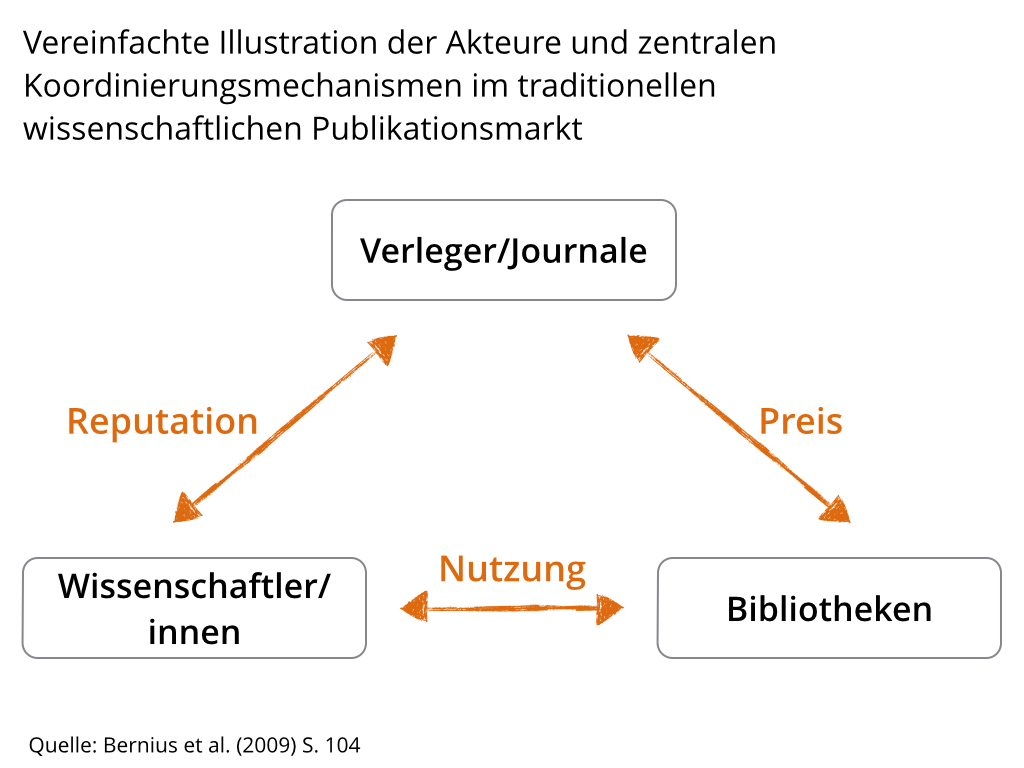
\includegraphics{url:https://github.com/christianheise/offene-doktorarbeit/raw/master/images/figure_publikationsmarkt_22915_1137.png}
\caption{Vereinfachte Illustration der Akteure und zentralen Koordinierungsmechanismen im traditionellen wissenschaftlichen Publikationsmarkt nach \cite{cite:21a}}
\end{figure}

Bernius et al. unterscheiden drei aufeinandertreffende koordinierende Marktmechanismen: die Reputation, die Nutzung wissenschaftlicher Publikationen, sowie den Preis für den Erwerb der Publikation \cite{cite:21a}. Während die Reputation ein non-monetärer Aushandlungsmechanismus zwischen wissenschaftlichen Verlagen und wissenschaftlichen Autoren ist, findet die monetäre Preisdefinition direkt zwischen Bibliotheken und Verlagen statt \cite{EuropeanCommission_sciencepub_2006}. Der monetäre Aushandlungsprozess zwischen Wissenschaftlern und Bibliotheken wird durch die Bedeutung und Nutzung der jeweiligen Publikation bestimmt \cite{cite:21a}. Nicht jede Publikation hat diesbezüglich die gleiche Wertigkeit \cite{suchen} und damit den gleichen Einfluss auf die Reputation eines Autors.

Zusammenfassend lassen die neuen Möglichkeiten der Verbreitung von Informationen einen vergleichbaren Veränderungsprozess der wissenschaftlichen Reputation und damit auch Anerkennung vermuten, wie er durch die Entwicklung des Buchdrucks ausgelöst worden war \cite{hanekop_2006}.

\subsubsection{Messbarkeit wissenschaftlicher Qualität und Publikationsquantität}

Wissenschaft ist ein Prozess, bei dem aus “unterschiedlichen Inputfaktoren, mittels verschiedener Transformationen Beiträge zur Schaffung neuer wissenschaftlicher Erkenntnisse als Output entstehen” \cite{Jansen_2007}. Die Messung und Bewertung des jeweiligen Outputs führt zur Aussage über die Performanz des jeweiligen Forschungsprozesses. Neben den Indikatoren für den Output wissenschaftlicher Performanz, müssen aber auch intermediäre Aspekte berücksichtigt werden \cite{schmoch_2009}.

Mit Beginn des 20. Jahrhunderts wurden in der Wissenschaftsforschung Indikatoren überwiegend zur Beschreibung der exponentiellen Wachstumsverläufe von Wissenschaft entwickelt und eingesetzt \cite{Hornbostel_1997}. In der Zeit nach dem zweiten Weltkrieg etablierten sich erstmals Indikatoren für die Effizienzmessung wissenschaftlicher Wissensproduktion und -verbreitung, die aber "ebenso wie Sozial- und Wirtschaftsindikatoren keine neutralen Realitätsbeschreibungen" \cite{Hornbostel_1997} darstellten. Spätestens seit den 1970er Jahren werden diese Messungen, die die Forschungsleistung quantifizieren sollen, flächendeckend durchgeführt \cite{Hornbostel_1997} um Forschungsqualität und Quantität quantifizierbar zu machen.

Seit den 1990er Jahren ist diese Bewertung von Wissenschaft in Gestalt von Zahlen als unkontrollierte Nebenprodukte digitaler Wissenskommunikation erweitert worden \cite{angermueller_2010}. Heute zählen in der Wissenschaft vor allem die wissenschaftliche Reputation und die als "Impact" bezeichnete Wirkung wissenschaftlicher Publikationen \cite{herb_open_2013} \cite{Hornbostel_1997}. Die Wirkung der wissenschaftlichen Kommunikation wird , wie im Kapitel "Wissenschaftliche Kommunikation" ausgeführt, anhand der quantitativen Betrachtung der Zitationen der jeweiligen Publikation ermittelt \cite{Brembs_2013} \cite[:16]{haustein_2012_multidimensional} \cite{weller2011twitter}. Diese rein quantitative Betrachtung muss allerdings auch als Proxy für die Bewertung von Wirkung in der "publish or perish" community verstanden werden \cite{peters_2015_research}.

Diese Art der Betrachtung basiert auf der Grundannahme, dass Kommunikation die "Essenz der Wissenschaft" \cite{bonitz_1998_matthaus} ist und "Zitierungen in ihrer Gesamtheit so etwas, wie die Grundelemente eines weltweiten Expertensystems" \cite{bonitz_1990_sci}. Nach dieser Sichtweise stellt eine häufige Zitation einen wesentlichen Indikator für die Wirkung der wissenschaftlichen Arbeit dar \cite{hamilton_1990_publishing}. Ein generalisierter und überzeitlicher Begriff von Qualität wissenschaftlicher Arbeit scheint nicht möglich, weil eine grundlegende Definition der Wissenschaftsindikatoren sowie ihrem Ziel der "Abbildung eines Konstrukts, das die Bewertungen einzelner Wissenschaftler oder Experten transzendiert" nicht möglich erscheint \cite{Hornbostel_1997}.

In den letzten Jahren haben sich neue Möglichkeiten für die Qualitätssicherung und -bewertung herausgebildet \cite{rekdal_2014_academic}. Die "Anforderungen an Verfügbarkeit von Dokumenten und Transparenz der Begutachtungen" der Open Access Bewegung haben die Frage aufgebracht, "ob möglicherweise Veränderungen der Review-Praktiken notwendig sind, um exzellente Wissenschaft zu identifizieren und vor allem zu fördern" \cite{suchen_Hornbostel_2006}. Des Weiteren stellt sich die Frage, ob die Berücksichtigung neuer Metriken für die Bewertung wissenschaftlicher Qualität eine Antwort auf die Herausforderungen in dem etablierten Messsystem von wissenschaftlicher Qualität und Publikationsquantität sein können.

Bestand die klassische Wirkungsmessung von Wissenschaft in der Ermittlung der Anzahl von Zitationen, ermöglichen die veränderten Bedingungen von wissenschaftlicher Kommunikation im Rahmen der Digitalisierung alternative Erhebungsmöglichkeiten der Wirkung formeller wissenschaftlicher Kommunikation und damit auch für die Erlangung wissenschaftlicher Qualität und Reputation. In den letzten Jahren wurde es viel einfacher, Fälle von Plagiaten und wissenschaftliches Fehlverhalten zu identifizieren, und auch andere Arten akademische Abkürzungen zu entdecken und zu sehen, wie erschreckend häufig sie auftreten \cite{rekdal_2014_academic}.

Ergänzend zu den etablierten zitationsbasierten Metriken spielen zunehmend detailliertere Analyse von nutzungsbasierten Metriken und Metriken Basis von Social Indikatoren \cite{peters_2015_research} bei der Bewertung von wissenschaftlicher Kommunikation eine Rolle. Die Befürworter solcher alternativer Metriken erhoffen sich von diesen neuen Verfahren eine unmittelbare, umfassendere und detailliertere Wirkungsmessung wissenschaftlicher Kommunikation und eine gerechtere Verteilung von wissenschaftlicher Reputation \cite{peters_2015_research} \cite{cite:17} \cite{dora_2013}.

\subsubsection{Wissenschaftliches Kapital}

Die Wissenschaft ist ein soziales Feld, dessen Strukturen und Praktiken das bestimmen, was in dem Kommunikations- und Publikationssystem als Wissenschaft und als wissenschaftliches Ergebnis gilt \cite{mikl_2010_soziologie}. Im Rahmen der Betrachtung von Steuerungs- und Reputationsmethoden für die Wissenschaft ist der Begriff "wissenschaftliches Kapital" von herausragender Bedeutung \cite{Barl_sius_2008}. Wissenschaftliches Kapital kann als eine Ausprägung des kulturellen Kapitals und als symbolisches, beziehungsweise non-monetäres Kapital \cite{irmer2011} \cite{hagner_2015_sache_buches} \cite{bourdieu_1988_homo} verstanden werden.

Piere Bourdieu sieht in der Wissenschaft ein soziales System und beschreibt es als angetrieben von dem ständigen Machtkampf um die Erlangung und Erhaltung von symbolischem Kapital \cite{bourdieu_1988_homo}. Dieser von Piere Bourdieu beschriebene Homo Academicus ist durch Selbstdisziplin, eine sehr ausgeprägte Neugier und die Fähigkeit Forschung und Lehre zu betreiben, charakterisiert \cite{bourdieu_1988_homo}. Das symbolische Kapitel als Antreiber seines Handelns wird in diesem Zusammenhang von der Sozilogin Mikl-Horke als Besitz an symbolischen Gütern beschrieben, "der besonders in einer Gesellschaft, die auf die Kooperation aller angewiesen ist, sehr kostbar ist" \cite{mikl_2010_soziologie}. Eine genauere Betrachtung dieses wissenschaftlichen Kapitals ist für das Verständnis der Motivation von Wissenschaftlern zu publizieren und zu kommunizieren, sowie für die Herausarbeitung der Katalysatoren und Hindernisse für die Öffnung wissenschaftlicher Kommunikation demnach unabdingbar.

Die Gewährung wissenschaftlichen Kapitals basiert heute auf der Kooperation zwischen publizierenden Wissenschaftlern und Verlagen \cite{herb_2006}. Die Wissenschaftler befinden sich in einer Abhängigkeit von den Verlagen. Diese Abhängigkeit wird auch als "Faustischer Pakt" bezeichnet und hinterfragt \cite{hagner_2015_sache_buches} \cite{Parks_2002_acadamic_faust}. Den Pakt sind Wissenschaftler notgedrungen eingegangen, "um den Preis, dass Barrieren zwischen Autoren und Lesern aufgebaut wurden" \cite{hagner_2015_sache_buches}. "Wissenschaftliches Kapital" kann in diesem Zusammenhang als “Ergebnis einer Investition (...), die sich auszahlen muss” \cite{herb_2006} definiert werden. “Diejenigen, die diese Berechtigungsscheine in der Hand halten, verteidigen ihr 'Kapital' und ihre 'Profite', indem sie diejenigen Institutionen verteidigen, die ihnen dieses 'Kapital' garantieren.” \cite{Bourdieu_1992}

Der Soziologe Bordieu unterscheidet zwei Typen wissenschaftlichen Kapitals \cite{Bourdieu_1998}. Das Kapital, das auf der politischen und institutionellen Macht beruht und das andere, dass aus der rein wissenschaftliche Anerkennung resultiert \cite{mikl_2010_soziologie}. Das Institutionelles wissenschaftliches Kapital weist die "Macht und die Erwartung zu, auf Institutionen und Organisationen der Wissenschaft einzuwirken und über die Produktionsmittel der Wissenschaft zu disponieren" \cite[:257]{Barl_sius_2008}. Es ist disziplinunabhängig und fachübergreifend. Das reine wissenschaftliche Kapital muss disziplinspezifisch erarbeitet werden und wird durch die Publikation von Inhalten in der jeweiligen Fachdisziplin hoch angesehenen Zeitschriften, bei besonderen Verlagen oder durch die Arbeit in reputierlichen wissenschaftlichen Einrichtungen erlangt \cite[:257]{Barl_sius_2008}.

Zitationsindexe sind Indikatoren für das wissenschaftliche Kapital, das durch Anerkennung entsteht \cite{Bourdieu_1998}. Die wissenschaftliche Reputation, die aus dem wissenschaftlichen Kapital resultiert, basiert auf der Liste der Publikationen in hoch gerankten Journalen und angesehenen Verlagen \cite{herb_2010}. Diese Bewertung ist klar symbolischer Natur und basiert "auf der Anerkennung und dem Kredit (...), den die Gesamtheit der Wettbewerber innerhalb des wissenschaftlichen Feldes gewähren" \cite{Bourdieu_1998} \cite{Barl_sius_2008} \cite{herb_2010}.

Das wissenschaftliches Kapitel ist dabei zunehmend der Kapitalisierung von Wissenschaft ausgesetzt, bei der um den Einfluss der Ökonomie und den "wissenschaftswidrigen Verwertungsdruck"  \cite[:12]{Neidhardt_2006} gerungen wird. Als ein Indikator dafür ist die Kopplung des wissenschaftliches Kapitals und an die output-orientierte Anreizsysteme zu verstehen. Diese Fokusierung auf die "Kenngrößen führt dazu, dass Wissenschaftlerinnen und Wissenschaftler einen Anreiz haben, sich weniger als Homo academicus, sondern eher als Homo strategicus zu verhalten und sich auf die gut messbaren Aufgabenbestandteile zu konzentrieren" \cite{Frost_2014}. Ein Beispiel ist die zunehmende Relevanz des Performanzindikators "Drittmittel" \cite{Fabrizio_2008} \cite{Jansen_2007}, bei dem neben der Sicherung der Qualität von Forschung und Lehre zunehmend direkte finanzielle und administrative Kontrolle eine Rolle spielt \cite{Barl_sius_2008}. Dem Drittmitteleinkommen wird als Indikator für Forschungsleistung eine hohe Bedeutung zugemessen \cite{Jansen_2007}. Daraus entsteht die Tendenz, das nicht nur die Erwartungen an die Bewertung von Wissenschaft sehr ambitioniert sind, sondern auch, dass die Interessen privater und öffentlicher Drittmittel-Auftraggeber in den Vordergrund rücken und die Unabhängigkeit von Wissenschaft und Forschung gefährden.

Ähnliches ist im Rahmen der stetigen Ökonomisierung des internationalen Universitätsbetriebes \cite{brembs2015open} und bei der leistungsbezogenen Mittelzuweisungen an die Universitäten zu beobachten \cite[:12]{Neidhardt_2006}. Vor allem die Verknüpfung von wissenschaftlicher Reputation mit der damit einhergehenden Verteilung von Mitteln und Stellen stellt eine neuartige Herausforderung an das Wissenschaftssystem dar, dessen Währung ursprünglich nicht Geld war \cite{hanekop_2006}.

Die Auseinandersetzung mit dem wissenschaftlichen Kapital im Rahmen der Forderung nach Öffnung wissenschaftlicher Kommunikation kann auch deshalb als wichtig erachtet werden, weil diese bisher nur begrenzt der wissenschaftlichen Logik folgt und eher auf einer "feldunabhängigen Logik der Akkumulation von Kapital" basiert \cite{herb_2006}. Mit der Zunahme an output-orientierten Anreizsystemen im deutschen Wissenschaftssystem \cite{osterloh2008anreize} und einem Ungleichgewicht in der Kooperation zwischen wissenschaftlicher Kommunikation und wissenschaftlichem Kapital wird diese Entwicklung bei der weiteren Betrachtung der Motivationsfaktoren für Veränderungsprozesse in der wissenschaftlichen Kommunikation eine wichtige Rolle spielen.

\subsection{Wissenschaftliches Ethos}

Das wissenschaftlichen Ethos hat die Funktion der Wissenschaft "eine soziale und politische Legitimationsbasis zu verschaffen" \cite{descher_2012_ethos}. Generell stellt die Verfügbarmachung von Forschungsergebnissen einen integralen Bestandteil des wissenschaftlichen Ethos dar \cite{Fangerau_2014}. Dabei wird "die moderne Wissenschaft als Methode und Praxis der Wissensbildung wird durch ein Ethos epistemischer Rationalität geleitet" \cite{Oezmen_2015}. Als "selbstregulatives und nach eigenen Regeln operierendes System muss sie ihren Ethos jeder neuen Generation vermitteln" und "Verantwortungsstrukturen und Rahmenbedingungen" schaffen, "die langfristig eine verlässliche Kultur wissenschaftlicher Integrität stärken" \cite[:7]{wr_2015_wissenschaft_integritaet}.

Der US-amerikanische Soziologe Robert K. Merton stellte diesen und weitere Grundprinzipien als normative Grundstruktur des Ethos von Wissenschaft vor \cite{Merton_1985}. Diesem Ethos liegt auch den Annahmen zu Grunde, dass es Vorteile für die wissenschaftliche Gemeinschaft bringt, wenn Daten zweitverwertet werden und dass Daten ein wirtschaftliches Gemeingut sind, deren Wert durch breitere Nutzung verbesser wird \cite{RIN_2010_open_research}. Darüber hinaus sind "systematische Widerspruchsfreiheit, interne Kohärenz, Klarheit, aber auch Sparsamkeit und Eleganz, Genauigkeit und Überprüfbarkeit" weitere integrale Bestandteile des Ethos \cite{Oezmen_2015}. Dabei gilt es auch dem Umstand Rechnung zu tragen, dass Wahrheit relativ ist und sich die Richtigkeit einer wahren Aussage nur mit Hilfe der genauen Bedingungen beschreiben lässt, unter denen sie wahr ist. Karl Raimund Popper attestiert der Wissenschaft demnach eine grundsätzliche "Fehlbarkeit" und leitet daraus ab, dass jedwede wissenschaftliche Erkenntnis möglichst offen für Kritik sein muss \cite{popper_2005_logic}.

"Anspruchslosigkeit und Bescheidenheit" sind weitere Grundtugenden des modernen Wissenschaftlers \cite{hagner_2015_sache_buches}. Das Ethos wird in diesem Zusammenhang als "Komplex von Werten und Normen" \cite{suchen} beziehungsweise "Verhaltensmaßregeln" \cite{suchen} verstanden. Merton unterteilt die Kriterien in die Kategorien, die alle auf das wissenschaftliche Kommunikationssystem anwendbar sind  \cite{Fröhlich_oa_2009}:
\begin{itemize}
\item \textit{Universalismus}: Die Geltungsansprüche der Wissenschaft sind allgemein und objektiv \cite{Oezmen_2015}. Die sozialen Merkmale eines Wissenschaftlers, wie zum Beispiel Nationalität, Geschlecht, Religion, Klasse usw. dürfen nicht in die Evaluation wissenschaftlicher Ergebnisse einfließen \cite{suchen}.
\item \textit{Kommunismus (Kommunalität)}: Es gibt eine Pflicht zur Veröffentlichung der Ergebnisse von Wissenschaft und Forschung und sie sind als Allgemeingut zu betrachten. Die wissenschaftliche Anerkennung und das Ansehen sind einziges damit verbundenes "Besitzrecht" \cite{suchen}.
\item \textit{Uneigennützigkeit}: Intrinsische "Neugier"\cite{suchen}, "selbstloses Eintreten für das Wohl der Menschheit"\cite{suchen} und der Wissensdurst müssen die vornehmlichen Motivatoren für Wissenschaftler darstellen \cite{suchen}.
\item \textit{Objektivität und Desinteresse}: Wissenschaft erfordert "Objektivität und Desinteresse" an den Ergebnissen der eigenen Forschung \cite{suchen} unabhängig von finanziellem Erfolg und Prestige \cite{suchen}. Wissenschaft nicht durch die persönlichen Präferenzen oder eigennützigen Motive und subjektiven Meinungen geleitet, sondern durch reines Erkenntnisinteresse und durch Wahrheit \cite{Oezmen_2015}.
\item \textit{Organisierter Skeptizismus}: Zweifel muss als "grundsätzliches Denkprinzip der Wissenschaft" \cite{suchen} und die "unvoreingenommene Prüfung und Kritik an Wissenschaft, Forschung und Autorität" \cite{suchen} als Kernbestandteil des Systems verstanden werden. Zum Beispiel gilt es den "Matthew Effect" zu vermeiden. Der Matthäus-Effekt ("Wer hat, dem wird gegeben" Mt. 25,29) ist ein Phänomen auf der Makroebene der Wissenschaft \cite{bonitz_1998_matthaus} und  beschreibt den Umstand, dass Autoren oder Publikationen, die bereits eine hohe Zitationsrate vorweisen können, meist noch häufiger zitiert werden als die Autoren oder Beiträge mit einer geringeren Zitationsrate. Überproportional profitieren in diesem System also die, die besonders häufig zitiert wurden \cite{Merton_1968} \cite{meier_2009_matthaus}.
\end{itemize}

Als Folge dieser Kriterien erkannte Merton das Urheberrecht an wissenschaftlichen Ideen und Beiträgen an, allerdings nur insofern, als dass das Urheberrecht allein auf die Ermöglichung der Anerkennung durch Kollegen und die Achtung der Priorität beschränkt bleibt \cite{Fangerau_2014}. Damit kritisiert er implizit das System der wissenschaftlichen Kommunikation.

In Folgeschriften kritisierter er darüber hinaus die neueren Konzepte und Praktiken, die "die Werte des klassischen Wissenschaftsethos korrumpieren" \cite{Fröhlich_oa_2009}. Inwieweit die aktuelle Wissenschaftspraxis von Mertons formulierten Werten abweicht, welche neue oder anderen Werte die wissenschaftliche Praxis mittlerweile beeinflussen und welchen Einfluss die neue Medientechnologien darauf haben, wird an anderer Stelle der Arbeit noch mal thematisiert.

Neben der internen wissenschaftlichen Verantwortung, die eng mit der der Regel guter wissenschaftlicher Praxis und offener wissenschaftlicher Kommunikation zusammenhängt, kann eine Ergänzung dieses Zusammenhangs um eine externe Verantwortung "im Sinne der Rechenschaftspflicht für die möglichen Anwendungen und Folgen seiner Forschung" \cite{Oezmen_2015} stattfinden. Sie ist zwar kein konstitutiver Bestandteil des Ethos der Wissenschaft, aber ein Teil einer Ethik der Wissenschaft \cite{Oezmen_2015}. In Verbindung mit der Forderung nach Öffnung der wissenschaftlichen Kommunikation ist aber dennoch zu berücksichtigen, dass die Verteidigung der Autonomie und Freiheit der Wissenschaft "nicht mit der ganz andersgelagerten These der Autarkie der Wissenschaft verwechselt" werden darf und mit "ethischen Zwecksetzungen eine Verletzung des epistemischen Ethos sowie eine Gefährdung der Autonomie der Wissenschaft befürchtet werden" kann \cite{Oezmen_2015}.

Der Umstand dar, dass die zunehmende Berücksichtigung bibliometrische Indikatoren anstatt der tatsächlichen Qualität der Wissenschaft im Rahmen der Steuerung von Wissenschaft zu negativen Auswirkungen auf normative Grundstruktur des Ethos der Wissenschaft haben kann, stellt einen weiteren Anknüpfungspunkt für die Herausforderungen im aktuellen wissenschaftlichen Kommunikationssystem dar.

\subsection{Wissenschaftlicher Diskurs}

\begin{quote}Wissenschaftliche Kommunikation vollzieht sich in Behauptungen, Erklärungen, Prognosen; sie ist nicht nur ein Informationsaustausch. Vielmehr vollzieht sich im wissenschaftlichen Diskurs der kollektive Prozess des wissenschaftlichen Begreifens. Deshalb ist die wissenschaftliche Sprache als Diskurs nicht bloß ein Medium der Kommunikation, sondern der Ort, an dem sich ein wesentlicher Teil der wissenschaftlichen Arbeit vollzieht, der kollektive Darstellungsraum der Wissenschaft. \cite{bohme_1978_wissenschaftssprachen}\end{quote}

Ebenso muss auch die Erforschung wissenschaftlicher Fragestellungen als ein zentraler Bestandteil des wissenschaftlichen Diskurses \cite{suchen} betrachtet werden. Die Verarbeitung von Forschungsergebnissen, die Anwendung und Neuinterpretation von Ergebnissen sowie das Verfassen von Gegenentwürfen und synthetischer Gesamtdarstellungen stellen Faktoren für den wissenschaftlichen Diskurs dar \cite{suchen}. Jürgen Habermas unterscheidet hier das kommunikatives Handeln von strategischem Handeln. Im dem "rationalen Diskurs" findet dabei vor allem eine Verständigung über problematische Geltungsansprüche statt \cite{suchen}. Der Beobachter entwickelt Methoden und Verfahren um zu einer Verständigung mit seiner Zielgruppe zu kommen \cite{suchen}. Der wissenschaftliche Diskurs operiert in diesem Verständigungsprozess funktional eigenständig und alles, was durch Wissenschaft kommuniziert wird, ist “entweder wahr oder unwahr” \cite{Luhmann1998}.

Michel Foucault versteht unter einem Diskurs "eine Menge von Aussagen, die einem gleichen Formationssystem zugehören"\cite{foucault_archaologie_1981}. Der wissenschaftliche Diskurs gründet sich demnach nur zum Teil auf die Forschung und kann auch nicht nur als "Kontaktglied zwischen dem Denken und dem Sprechen" \cite{foucault_ordnung_2003} definiert werden. Er wird getrieben vom Willen zur Wahrheit, der sich durch "die Pädagogik, dem System der Bücher, der Verlage und Bibliotheken, den gelehrten Gesellschaften einstmals und den Laboratorien heute" ständig erneuert \cite{foucault_ordnung_2003}. Abgesichert wird der Diskurs "durch die Art und Weise, in der das Wissen in einer Gesellschaft eingesetzt wird, in der es gewertet und sortiert, verteilt und zugewiesen wird" \cite{foucault_ordnung_2003}. In der foucault'schen Diskursanalyse wird der Diskurs als die Fähigkeit definiert, die "Beziehungen" zwischen "Institutionen, ökonomischen und gesellschaftlichen Prozessen, Verhaltensformen, Normsystemen, Techniken, Klassifikationstypen und Charakterisierungsweisen herzustellen" \cite{foucault_archaologie_1981}.

Im Rahmen des wissenschaftlichen Diskurses versuchen Menschen mit diversen "Machtprozeduren", die "ungeordnete und wuchernde Masse aller Äußerungen" zu reglementieren und zu kontrollieren \cite{Neymeyer_diskurs_2010}. Resultierend daraus entstehen Diskurse, die sich über einen gemeinsamen Gegenstand definieren. Sie gehorchen "impliziten wie expliziten Regeln", unterliegen "spezifischen Funktionen", nehmen bestimmte Formen an und sind von "Machtmechanismen gekennzeichnet" \cite{Neymeyer_diskurs_2010}. Diese grundlegende Definition des Diskurses ist für die weitere Betrachtung der Veränderungsprozesse und die Forderung nach Öffnung der wissenschaftlichen Kommunikation unabdingbar.

Die Forderungen um die Öffnung wissenschaftlicher Kommunikation beruhen auf der Annahme, dass sie die Grundlage dafür schaffen, dass wissenschaftliche Diskurse besser und umfassender geführt werden können, als im aktuell bestehenden System. Nach der klassischen Einordnung ist damit aber nicht eine Öffnung des Diskurses außerhalb der wissenschaftlichen Gemeinschaft gemeint, sondern nur die Senkung der Zugangsbarrieren zu wissenschaftlicher Kommunikation. Das Ziel des Ausschlusses der Öffentlichkeit aus den wissenschaftlichen Diskursen liegt darin, die Macht sowie Auswüchse des Diskurses einzugrenzen, seine Ergebnisse zu bändigen und das Wissen durch den "Willen zur Wahrheit" \cite[:15]{foucault_1991_ordnung} zu kanalisieren.

\section{Die Forderung nach Öffnung der wissenschaftlichen Kommunikation}

Wie dargestellt, steht das wissenschaftliche Kommunikationssystem vor mannigfaltigen Herausforderungen. In folge der zunehmenden Privatisierung wesentlicher Bestandteile des wissenschaftlichen Kommunikationsprozess, haben sich die akademischen Ziele und die Marktinteressen der privatwirtschaftlichen Anbieter immer weiter voneinander entfernt. Zum Beispiel sind im Zeitraum von 1986 bis 2012 die Ausgaben für Bibliotheksbestände in den Vereinigten Staaten um 322 Prozent gestiegen \cite{lewis_2015_future}. Den Verlegern werden Betriebsgewinnmargen von über 35 Prozent \cite{russell_2008_business} \cite{cope2014future} sowie hohe jährliche Wachstumsraten \cite{Martin_2013} \cite{Wellcome_Trust_2003}. Die drei größten Wissenschaftsverlage vereinen bereits 42 Prozent aller Journale und trotz der internationalen Finanzkrise stiegen die Umsätze ungebremst weiter. In den Jahren zwischen 2008 und 2011 stiegen die Umsätze um 11,7 Prozent und die Gewinne von 1,6 Milliarden auf 1,9 Milliarden Dollar (17 Prozent) \cite{cope2014future}. Das entspricht einer Umsatzrendite von 35,8 Prozent. Im Vergleich dazu lagen die durchschnittlichen Umsatzrenditen im Wirtschaftszweig "Verlagswesen" bei deutschen Firmen mit mehr als 50 Mitarbeitern lag laut der Bundesbank dem im Jahr 2011 bei 11,6 Prozent \cite{bundesbank_2014}. Es sind nur wenig Beispiele bekannt, "in denen das symbolische Kapital in so außerordentlichem Maße zu ökonomischen Kapital verdinglicht worden ist", wie bei dem Geschäftsmodell des wissenschaftlichen Publizierens \cite{hagner_2015_sache_buches}.

Als möglicher Ausweg aus dieser Krise wird immer wieder die Digitalisierung und Öffnung der wissenschaftlichen Kommunikation durch Konzepte wie Open Access und Open Science genannt \cite{lewis_2015_future}. Beide Begriffe umfassen eine Vielzahl von Möglichkeiten für die Zukunft der Wissensbildung und Wissensverbreitung. Sie funktionieren als Sammelbegriffe für unterschiedliche Auffassungen wie weit und in welcher Form Wissenschaft offener werden kann. Sie sind Bestandteil eines notwendigen Diskurses in der wissenschaftlichen Gemeinschaft \cite{schulze_2013_open}. Kleinster gemeinsamer Nenner in diesem Diskurs um die unterschiedlichen Konzepte ist, "dass wissenschaftliche Forschung sich irgendwie mehr öffnen muss" \cite{cite:9}.

Rainer Kuhlen definierte diesbezüglich schon 2002 drei Szenarien wie der Zugriff auf Wissen in Zukunft organisiert werden könnte \cite{Kuhlen_2002_universalaccess}:
\begin{enumerate}
\item Elektronische Informationen sind frei zugänglich und die Konzepte der individuellen Autorenschaft und des geistigen Eigentums werden zu Relikten aus bürgerlichen Vorinformationsgesellschaften
\item Wissen und Informationen sind kontrolliert und dem Markt ohne politische Gegensteuerung überlassen: Die Kommerzialisierung und Zonierung von Wissen und Information wird umfassend sein und den Alltag bestimmen.
\item Wissen und Information werden über koexistente oder Paralleluniversen organisiert: Das Wissens als Produkt ist frei, öffentlich zugänglich und nutzbar. Es bleibt aber genug Spielraum bei der Adaption, Beratung, Veredlung oder anderen Mehrwertleistungen einer kommerziellen Informations- und Wissenswirtschaft
\end{enumerate}

Aktuell stehen die etablierten Prozesse wissenschaftlicher Kommunikation vor umfangreichen Herausforderungen. Die Zeitschriften- und Monographienkrise, der zunehmende finanzielle Druck im Rahmen der öffentlichen Finanzierung von Wissenschaft, die Veränderungen im wissenschaftlichen Kommunikationsprozess durch neue Arten und Möglichkeiten der Distribution, die steigenden Beschaffungskosten für wissenschaftliche Literatur \cite{cite:17} \cite{muller_2010_open}, sowie die Veränderungen in der Rezeption von Inhalten \cite{holub_2013_reception} zwingen zum Umdenken in der wissenschaftlichen Kommunikationspraxis \cite{suchen}. Die anhaltende Forderung nach mehr Offenheit im wissenschaftlichen Kommunikationsprozess entwickelte sich zu einem konkreten Lösungsansatz für die Herausforderungen an das etablierte System.

Die Öffnung der wissenschaftlichen Kommunikation ist eine große Chance für Veränderungen im wissenschaftlichen Qualitäts- und Reputationssystem zu erwirken. Bisher werden wissenschaftlichen Erkenntnisse häufig erst nach langen intransparenten Verfahren bewertet, publiziert und nur an einen beschränkten Kreis von Rezipienten vermittelt. Diese intransparente Praxis hat einen signifikant-negativen Einfluss für Allokation von Ressourcen durch die öffentliche Hand und die Kosten die im Rahmen öffentlich-finanzierter Forschung entstehen. Die Öffnung der wissenschaftlichen Kommunikation würde demnach entgegen der bisherigen Praxis eine stärkere Berücksichtigung der Aspekte Aktivität der Wissenschaftler und die Qualität der Forschungsergebnisse ermöglichen \cite{suchen}.

Als Auslöser für die Entwicklung von Open Access werden auch die infrastrukturellen Veränderungen angeführt, die "seit spätestens Mitte der 1990er-Jahre entscheidend Einfluss auch auf die Wissenschaftskommunikation und das wissenschaftliche Arbeiten genommen haben" \cite{schulze_2013_open}. Open Access entwickelte sich vorerst primär in den STM-Fächern, in denen viel Aufmerksamkeit auf der Selbstarchivierung der Wissenschaftler und Wissenschaftlerinnen vor der finalen Publikation (Pre-Print) in privaten, zentralen oder institutionellen Repositorien lag \cite{adema_2013_political} und bei denen die Auswirkungen der Zeitschriftenkrise am stärksten zum Tragen kam \cite{naeder_2010_open}. Wissenschaftliche Informationen werden seither nicht nur in "digitaler Form konsumiert, sondern auch kollaborativ und kooperativ, zeitlich versetzt, durch teilweise räumlich weit verstreute Arbeitsgruppen und Forschungsverbünde, genutzt und weiterverarbeitet" \cite{schulze_2013_open}. Die Verbreitung und Akzeptanz von Open Access variiert dabei zwischen den einzelnen wissenschaftlichen Disziplinen erheblich \cite{cite:21a}.

In der Debatte über die Zukunft des wissenschaftlichen Publizierens und Kommunizierens besteht die Tendenz, Konzepte der offenen Wissenschaft als einen bisher beispiellosen und noch nie dagewesenen Wandel darzustellen \cite{cite:17a} \cite{cite:17b}. Diese Haltung basiert auf "verschiedenen Gründungsmythen", die auf "unterschiedliche Zielsetzungen und Lösungspfade" verweisen \cite{suchen-Hoffmann-Zugang-undVerwertung-oeffentlicher-Informationen}. Die Geschichte von Open Access ist eine Entwicklung, die unter anderem eng mit der Digitalisierung von Kommunikationsprozessen auf der einen, sowie mit der Zeitschriftenkrise auf der anderen Seite verknüpft ist \cite{suchen-Hoffmann-Zugang-undVerwertung-oeffentlicher-Informationen} \cite{yiotis_2013_open} \cite{wein_2010_erwerbung}. Open Access ist kein Selbstzweck \cite{cite:17d}, sondern ein Attribut tiefergehender Prozesse, die mit der wachsenden Bedeutung der Digitalisierung in unserer Zivilisation und dem damit einhergehenden Wandlungsprozessen im Machtgefüge zusammenhängen \cite{cite:17e}. Es bleibt jedoch herauszuheben, dass es trotz vereinzelter Versuche, wissenschaftliche Informationen und Publikationen offen und frei zu kommunizieren, Open Access im Printzeitalter physisch und ökonomisch über lokale Grenzen hinaus schwer möglich war \cite{cite:18a}.

Die Forderung nach der Öffnung von Wissenschaft und Forschung ist in diesem Zusammenhang nicht nur eine "politische Reaktion" oder "technische Alternative", sondern eine "alternative Formatierungen einer wissenschaftlichen Infrastruktur im technischen, rechtlichen und zeitlichen Sinne" \cite{kelty_2004}. Diese Infrastruktur ist schwer zu erfassen \cite[:319]{bowker_2000_sorting}, und dennoch betreffen sie "Wissenschaftler, politische Entscheidungsträger und die Öffentlichkeit" \cite{Scheliga_2014}.

Bei der genauen Betrachtung dieser Forderungen nach Öffnung wissenschaftlicher Kommunikation ist es deshalb zwingend erforderlich die Konzepte von Open Access und Open Science abzugrenzen. Open Access bezieht sich einen möglichst uneingeschränkten Zugang zu finalen wissenschaftlichen Ergebnispublikationen für die Gesamtgesellschaft. Open Science beschreibt hingegen den umfassenden Zugriff auf den gesamten wissenschaftlichen Erkenntnisprozess inklusive aller Daten und Informationen, die bereits bei der Erstellung, Bewertung und Kommunikation der wissenschaftlichen Erkenntnisse entstanden sind.

\subsection{Wissenschaftliche Kommunikation als Open-Source-Prozeß}

Wenn es im aktuellen öffentlichen Diskurs um die Öffnung wissenschaftliche Informationen, Infrastruktur und Arbeiten geht, werden immer öfter Schlagworte mit dem Attribut „Open“, wie Open Access, Open Research und Open Science, verwendet \cite{bunz_2014} \cite{schulze_2013_open}. "Offen" ist dabei nicht mit "kostenlos" gleichzusetzen \cite{grand_2012_open} und bezieht sich üblicherweise auf zwei Kernaspekte: Zum einen die Offenheit des Zugangs zu wissenschaftlichen Text, Daten, Quellcode oder Ergebnissen und zum anderen auf das Gebot der Transparenz, also die Offenlegung, beziehungsweise der Zugriff auf Verfahren, Methoden und Ziele \cite{schulze_2013_open}. "Offenheit" (Openness) wird im Rahmen dieser Arbeit multidimensional adressiert. Sie hat eine rechtliche, wirtschaftliche, technische, politische, sowie eine kulturelle Dimension.

Im Rahmen der Forderung nach der Öffnung der wissenschaftlichen Kommunikation und wissenschaftlichen Publikationen werden in der Literatur immer wieder Vergleiche zur Open Source-Bewegung gezogen  \cite{cite:9} \cite{Peters_2014} \cite{RIN_2010_open_research} \cite[:423]{mantz_2007_open} \cite{cite:1}. Diese Vergleiche dienen dabei beispielhaft dem Verständnis theoretischer Grundlagen im Rahmen der Öffnung von Wissenschaft und Forschung.

Open Source ist ein Begriff aus der Softwareentwicklung, der als Gegensatz zum Verfahren der Wissenssicherung \cite{stallman2002} eine quelloffenen Handhabe von Programmcode beschreibt und in den 1990iger erstmals eingeführt wurde \cite[:5]{hippel_2003_open}. Dieser Begriff wird praktisch, auch wenn es philosophisch enorme Meinungsunterschiede gibt \cite[:5]{hippel_2003_open}  \cite[:169]{stallman2002}, synonym mit “freier Software“ (nicht Freeware) verwendet \cite{naeder_2010_open} \cite[:414]{mantz_2007_open}. Dabei folgt die Open Source-Entwicklung der Maxime, dass die Kernsteuerungsinformationen und -befehle (Quelltext) von Software öffentlich einsehbar und zugänglich sind, sowie je nach gewähltem Lizenzmodell modifiziert, kopiert oder weitergegeben werden können. Der Unterschied zu Stallmans "Free Software" besteht hauptäschlich darin, dass Open Source Software Produktion nicht zwangsläufig ausschließt das Produkt kommerziell gegen Bezahlung mit properitären Erweiterungen zu vertreiben, während Free Software prinzipiell immer frei verbreitet werden muss \cite{stallman2002}.

Bei der Open Source-Entwicklung veröffentlichen Programmierer den Code einer Software offen im Internet. Andere Programmierer haben jeweils die Möglichkeit, diesen Code so weiterzuentwickeln und anzupassen, wie es ihnen beliebt. Dadurch entsteht ein offenes Ökosystem an Software - womit nicht zwangsläufig ein fertiges Programm gemeint sein muss - , bei dem nicht mehr der Zugriff die Hürde darstellt sondern die Adaption oder der Einsatz der vorhandenen Lösungen. Diese Entwicklungsmethode unterscheidet sich zum traditionellen Modell der Entwicklung von Software mit der Feststellung, dass Open Source-Software das Prinzip der Exklusivität des geistigen Eigentums auf den Kopf stellt, weil diese Software "um das Recht auf Vertrieb konfiguriert, nicht auszuschließen ist" \cite{suchen}. Auch wenn noch immer nicht vollständig geklärt ist, ob Open Source Software wirklich "schneller, besser oder günstiger" ist, hat sich Open Source in den letzten Jahren stark verbreitet \cite{Lerner_2001} und an Bedeutung gewonnen.

Die Definition von Open Source beinhaltet festgelegte Kriterien für die Klassifizierung \cite{osd_2003}: Freie Weitergabe ohne zusätzliche Kosten, das Programm muss den Quellcode beinhalten und den Code offen zur Verfügung stellen, die verwendete Lizenz muss Derivate zulassen, die Unversehrtheit des Quellcodes des Autors muss garantiert werden, die Diskriminierung von Personen oder Gruppen muss ausgeschlossen sein, es darf keine Einschränkung des Einsatzfeldes geben, die Lizenz muss weitergegeben werden können und auf das Produktpaket anwendbar sein und die Lizenz darf die Weitergabe des Programmcodes zusammen mit anderer Software nicht einschränken.

Im Vergleich zum klassischen Softwareentwicklungsprozess definiert der Hamburger Wirtschaftsinformatiker Markus Nüttgens folgende charakteristische Merkmale \cite{nuttgens_2014}:
\begin{enumerate}
\item Anzahl der beteiligten Entwickler: Im Vergleich zu traditioneller Softwareentwicklung ist eine weitaus größere Anzahl von Entwicklern beteiligt. Es gibt es keine klare Grenze zwischen Entwicklern und Anwendern, da die Hürden für eine Partizipation im Entwicklungsprozess sehr gering sind. Auch wenn ein großer Teil der Entwicklungsarbeit von Freiwilligen übernommen wird, gibt es dennoch den Trend zum Einsatz bezahlter Entwickler.
\item Zuteilung der Arbeit: Im Open Source Programming (OSP) wird die Entwicklungsarbeit nicht länger von einer definierten Instanz zugeteilt, sondern die Teilnehmer wählen ihre Arbeitspakete selbst aus.
\item Architektur: In der Regel orientierten sich die Teilnehmer eines OSP nicht an einer vorgegebenen System-Architektur. Die Gestaltung der Architektur geschieht dezentral und ist oftmals häufigen Richtungswechseln unterworfen.
\item Koordination: Es gibt wenig oder keine institutionalisierten traditionellen Koordinationsmechanismen, wie z.B. Projekt- und Zeitpläne, Lasten- und Pflichtenhefte u.ä.” \cite{suchen}
\end{enumerate}

Um die Logik, Sprache, Begriffe, Kategorien und Operationen die die (neuen) Medien charakterisieren zu können, bedarf es eine Verknüpfung und tiefere Auseinandersetzung mit Informationstechnolgie \cite[:65]{manovich_2001_language}. Die Verknüpfung der Open-Source Entwicklungsmethode mit der Forderung nach Öffnung von Technologie, Bildung und wissenschaftlichen Kommunikation wurde unter anderem von dem Literaturwissenschaftler und Medientheoretiker Friedrich Kittler manifestiert \cite{cite:1}, der darin eine Chance für den anhaltenden Überlebenskampf der Universität sieht \cite[:7]{chun_2006_new}.

Open Source Entwicklungsprozesse weisen auch insofern Konvergenzen mit der Forderung nach der umfassenden Öffnung wissenschaftlicher Kommunikation auf, als dass es in beiden Fällen nicht nur um den freien und offenen Zugang zum finalen Ergebnis geht, sondern um die Möglichkeit des Zugriffs im gesamten Verlauf des Erstellungsprozesses \cite{kelty_2004}. Die Open Source Entwicklungsprozesse unterscheiden sich von den klassisch-traditionellen (closed-source) Softwareentwicklungsprozessen insbesondere durch die transparente Präsenz und permanente öffentliche Einsehbarkeit. Adaptiert man diese Open Source-Prozesse auf wissenschaftliche Erkenntnisprozesse und definiert in diesem Zusammenhang wissenschaftliche Publikationen als Quellcode, ist das Konzept auf den wissenschaftliche Erkenntnisprozess mindestens teilweise übertragbar \cite{garcia_2010_open} \cite{Singh_2008} \cite{Bradley_2008} \cite{mantz_2007_open} \cite{dorschel_2006_open} \cite{Bradley_2007} \cite{Willinsky_2005}. Dass das System der offenen Softwareentwicklung dem System der Erkenntnisgewinnung in der Wissenschaft ähnelt, beruht auch auf der Parallele, dass in der Wissenschaft neues Wissen auf der Grundlage von bereits vorhandenem und verfügbaren Wissen entsteht. Das gilt ebenso für Open-Source Entwicklungen, bei denen Entwickler und Entwicklerinnen häufig auf Softwareteile anderer zurückgreifen.

Ähnlichkeiten bestehen ebenso bei der Motivation für die Erstellung offener Software und für den wissenschaftlichen Erkenntnisgewinn. Zusammenfassend sind beide Prozesse in nachfolgend aufgelisteten Aspekten einander ähnlich:
\begin{enumerate}
\item Wie bei der wissenschaftlichen Kommunikation, baut die Entwicklung vieler Open Source Projekten auf den Inhalten, Steuerungsinformationen und Erfahrungen anderer Projekte auf. Die Projekte profitieren dabei von einem ständigen Austausch von Informationen, gegenseitiger Optimierung und Verbesserung. Wie bei Open Source Software streben auch Wissenschaftler nach der größtmöglichen Verbreitung ihrer Inhalte.
\item "Free Software (im Sinne von Open Source), Open Access und Creative Commons sind alles Rechts- und Infrastrukturexperimente"\cite{kelty_2004}. Open Source-Software sollte dabei nicht mit "Shareware" verglichen werden, die zwar kostenlos verbreitet wird, aber deren Quellcode proprietär bleibt \cite{Lerner_2001}
\item Die Kontributoren von Open Source Projekten versprechen sich neue "Karrieremöglichkeiten oder eine Ego-Genugtuung" \cite{Lerner_2001}, Selbstverwirklichung oder Befriedigung der intellektuellen Neugier \cite{Willinsky_2005}, sowie gegenseitige Beurteilung und Anerkennung (non-monetäres Kapital). Das wissenschaftliche System basiert auf ähnlichen Mechanismen beim Karriere- und Reputationssystem.
\item Parallelen ergeben sich auch auf der Nutzerseite: "Denn hier wie dort gilt es, das Spannungsfeld zwischen dem Prinzip des „offenen Zugangs“ auf der einen Seite und dem Wunsch mancher Urheber, die Nutzung seines Werkes – teils aus ideellen, teils aus ökonomischen Motiven – auf bestimmte „gewünschte“ Nutzungsformen zu beschränken" \cite{dorschel_2006_open}.
\item Wie bei der wissenschaftlichen Kommunikation, geht es bei der Mitarbeit an Open Source Projekten nicht ausschließlich um altruistische Motive \cite{Lerner_2001} und um kollektive bzw. arbeitsteilige Prozesse zur Wissensproduktion.
\item Die Debatte um die Forderung nach Öffnung der wissenschaftlichen Kommunikation kann aus technologisch-entwicklungsmethodischer Sicht mit der Debatte um kostenloser Software (Freeware) versus Open Source Software verglichen werden. Der Vergleich: Freeware und Open Access Publikationen sind zwar kostenlos verfügbar, ihr Erstellungsprozess wird jedoch nicht offen und transparent kommuniziert. Bei Open Science geht es wie bei Open Source um die Offenlegung des gesamten Erstellungsprozesses inklusive der Daten \cite{grand_2012_open} sowie auch den benutzten wissenschaftlichen Code \cite{hey_2015_open}.
\item Auch die häufig genutzten Lizenzmodelle und Definitionen von Offenheit im Rahmen wissenschaftlicher Kommunikation haben ihren Ursprung in der Open-Source-Bewegung \cite{suchen}.
\end{enumerate}

Der Vergleich der Öffnung von Wissenschaft mit der Open-Source Bewegung wird im Rahmen dieser Arbeit als ein Ansatzpunkt erachtet, um ein mögliches Szenario aufzuzeigen, wie in Zukunft die Wissensproduktion frei und öffentlich gestaltet werden kann. Dabei gilt es zu berücksichtigen, dass bei der Nutzung Open Access publizierter Werke und Publikationen die Erfahrungen aus dem Bereich der Open Source-Software dienlich sein können, wobei sich die die rechtlichen Fragestellungen und Lösungsansätze auf Anbieterseite doch zum Teil erheblich unterscheiden \cite{dorschel_2006_open}. Diese Einschränkung resultiert aus einer partiell differenten Interessenlage: OpenSource-Software basiert in hohem Maße auf dem Community-Gedanken und ist letztlich altruistischen Motiven geprägt, während bei Open Access zum Teil die Ressourcenknappheit der öffentlichen Hand sowie die individuellen Renommeeinteressen des Wissenschaftlers im Vordergrund stehen \cite{dorschel_2006_open}. Im Rahmen der Veränderungsprozesse und Ausweitung der Öffnung auf den gesamten wissenschaftlichen Erkenntnisprozesses muss diese Einschränkung der Vergleichbarkeit allerdings hinterfragt werden, was im weiteren Verlauf dieser Arbeit dargestellt wird.

\subsection{Die Forderung nach Öffnung der wissenschaftlichen Kommunikation}

Während "Openness" bisher vielfach mit den Entwicklungen im Zusammenhang mit offener Software assoziiert wird, gibt es Anknüpfungspunkte von "Offenheit" als Begriff in der wissenschaftlichen Auseinandersetzung, die schon zeitlich früher anzusetzen sind \cite{Tkacz_2014}. So sieht Christopher Kel­ty die ersten Anfänge bereits in den 1980er Jahren \cite{kelty_2008_two_bits}. Andrew Russell sieht die ideologischen Ursprünge von "Offenheit" als Standard schon in der Entwicklung des Telegraphs und weiteren Ingenieurleistungen seit 1860 \cite{Russell_2014}. Könneker und Lugger sehen erste Beispiele einer offenen Wissenschaft bereits im 17. Jahrhundert \cite{Konneker_2013}. Zu dieser Zeit herrschte noch keine strikte Trennung zwischen Wissenschaftlern und nicht-Wissenschaftlern und die "öffentliche Demonstrationen von Experimenten mit großem Überraschungs-und Unterhaltungswert beziehen das Publikum ein" \cite{weingart_2005_wissenschaft}.

Das aktuell vorherrschende System der wissenschaftlichen Kommunikation hat sich seit den 1960er Jahre etabliert und funktionierte am Besten, als die akademischen Ziele und mit den Marktinteressen vereinbar waren. Doch die Rahmenbedingungen wissenschaftlicher Kommunikation haben sich seitdem fundamental verändert \cite{epaa_Weiner_2001}. Infolge des weltweit steigenden Haushaltsdrucks der Bibliotheken und wissenschaftlichen Institutionen, des "ungewöhnlichen Geschäftsmodells" \cite{cite:12} der Wissenschaftsverlage mit immer höheren Margen \cite{albert_2006_open_implications}, der Massifizierung der Universität \cite{binswanger_2014_excellence}, des konstanten Anstiegs des wissenschaftliche Outputs \cite[:23]{haustein_2012_multidimensional} und des Umstandes, dass private Wissenschaftsverlage durch das wissenschaftlichen Reputationssystem über öffentlich finanzierte Wissenschaftlerkarrieren entscheiden \cite{heise_2012}, befindet sich das wissenschaftliche Kommunikationssystem in einer Krise \cite{cite:14}.

Im Rahmen der technologischen Entwicklungen bei der Digitalisierung des wissenschaftlichen Arbeitens und elektronischen Publizierens kann die Öffnung der wissenschaftlichen Kommunikation als eine mögliche Antwort auf diese Krise verstanden werden, setzt bei der Öffnung (Open) und dem freien Zugang (Access) zu wissenschaftlichen Publikationen an und könnte perspektivisch zu einer Öffnung (Open) des Zugriffs auf den Prozess des Forschens (Science) führen. Darüber hinaus werden wissenschaftliche Ergebnisse zunehmend zum Thema massenmedialer Berichterstattung, wodurch sich der ursprüngliche Publikumsbezug der wissenschaftlichen Kommunikation zur jeweiligen Fachgemeinschaft um den Bezug zur allgemeinen Öffentlichkeit ergänzt" \cite{bbaw_publizieren_2015} .

Dieser Wandel im "Zeitalter der Informatik", birgt aber auch Herausforderungen, die der Philosoph Jean-François Lyotard als "Ökonomisierung des Wissens" \cite{lyotard_1993_postmoderne} auch im Rahmen der zunehmenden Quantifizierbarkeit bezeichnet. Die Produktion von Wissen erfolgt demnach nicht mehr (nur) zum Zweck der Erweiterung des Wissens, sondern mit dem Ziel es zu verkaufen \cite[:156]{troy_2012_wissen}. Wie im Kapitel "Wissenschaftliches Kapital" beschrieben beruht die Produktion von wissenschaftlichem Wissen aber eben ursprünglich nicht auf den Marktmechanismen, sondern auf einem nicht-kommerzielle Anreizsystem und wird durch symbolisches Kapital angetrieben \cite[:157]{troy_2012_wissen}.

Aus der Öffnung der Kommunikation, so wird befürchtet, entsteht die Gefahr, dass wissenschaftliches "Wissen immer weniger der Bildung dient, sondern für den Verkauf geschaffen und konsumiert wird" \cite{hagner_2015_sache_buches}. Diese Gefahr beschreibt das Spannungsverhältnis in dem Wissenschaftler und Wissenschaftlerinnen auf der einen Seite zunehmend angehalten sind, die Forschung gemeinsam mit der Industrie schnell in Produkte zu übersetzen und auf der anderen Seite das Wissen so schnell wie in der wissenschaftlichen Gemeinschaft verbreitet werden soll, um den wissenschaftlichen Fortschritt zu fördern sowie um die gesellschaftlichen und humanitären Ziele von Wissenschaft zu erfüllen \cite{harmon_2012_commercialization} \cite{Woelfle_2011}. Diese Gefahr wird auch in der Debatte um die Öffnung wissenschaftlicher Kommunikation genannt \cite{Kansa_2014_open_neoliberalism} \cite{bunz_2013_open} \cite{tkacz_2012_open} \cite{mirowski_2005_contract} und wird im weiteren Verlauf der Arbeit aufgegriffen. Eine weitere Herausforderung stellt die Frage dar, ob und in wie weit durch die Öffnung der wissenschaftlichen Kommunikation massenmediale Selektionskriterien als Steuerungsmechanismen für Wissenschaft wirksam gemacht werden \cite{bbaw_publizieren_2015}.

Diese Veränderungen in der Kommunikation von Forschung und Wissenschaft sind keine völlig neue Phänomene, denn in gewisser Weise ist die Öffnung der wissenschaftlichen Kommunikationsprozesse eine Rückkehr zu der ursprünglichen Beziehung zwischen Wissenschaft und Öffentlichkeit \cite{Konneker_2013} \cite{weingart_2005_wissenschaft}.

In der gegenwärtigen Literatur kommen die Begriffe um "Offenheit" in der wissenschaftlichen Auseinandersetzung auf unterschiedlichste Art und Weise zur Anwendung \cite{cite:9}. Die Unterscheidung von "Zugang" und "Zugriff" erscheint dabei wesentlich und stellt eine der zentralen Grundlagen für die Abgrenzung der hier verwendeten unterschiedlichen "Open"-Begriffe dar:
\begin{itemize}
\item Offener "Zugang" bezieht sich auf einen unbeschränkten Zugang zur finalen wissenschaftlichen Publikation. Zugang meint das "das freie, unwiderrufliche und
weltweite Zugangsrecht" \cite{berliner_erklaerung_2003}. "Unbeschränkt" meint hier vor allem das ausschließliche Lesen der finalen Ergebnispublikation aber auch die Erstellung von Kopien, sowie Verarbeitung und Benutzung dieser \cite{Lossau_oa_2007} bei Nennung der Urheberschaft. Dieser Open-Access-Ansatz bezieht sich zunächst lediglich auf die Zugangsbedingungen zu den wissenschaftlichen Arbeiten \cite{muller_2010_open}. Dabei bezieht sich dieser Zugang auf einen Zeitpunkt, nach der Entwicklung und Veröffentlichung des bereits abgeschlossenen wissenschaftlichen Erkenntnisprozesses und die Publikation bereits eingereicht oder veröffentlicht wurde.
\item Offener "Zugriff" soll als erweiterte Nutzung der jeweiligen Wissensressourcen verstanden werden und schließt neben dem "Zugang" zur Publikation sämtliche Informationen und Daten, Quellcode, sowie die Kommunikation hinter und vor der finalen Veröffentlichung \cite{hey_2015_open} ein. Dieser Zugriff bezieht sich als Erweiterung zu den ersten Forderungen nach "Open Access" auch auf "Daten" als "Gesamtheit der binär codierten, maschinenlesbaren Inskriptionen" und "all das, was auf digitalen Datenträgern gespeichert vorliegt" \cite{Burkhardt_2015}. "Zugriff" beschränkt sich hier also nicht nur auf den reinen Zugang zu wissenschaftlicher Information im Rahmen des Publikationsprozesses, sondern schließt auch den Zugriff auf sämtliche Forschungsdaten, Methoden und wissenschaftlichen Begleitinformationen, die während der wissenschaftliche Arbeit auf dem Weg zur finalen Publikation entstehen ein und ermöglicht die Weiternutzung, Weiterverarbeitung sowie die Erstellung von Derivaten durch Dritte. Im Unterschied zum "Zugang" geht es dabei auch um einen "Zugriff" auf die Informationen der weit vor den Zeitpunkt der finalen Einreichung oder Publikation liegt und unmittelbar mit Beginn des wissenschaftlichen Erkenntnisprozesses beginnt.
\end{itemize}

\subsection{Offener Zugang zur wissenschaftlichen Kommunikation: Open Access}

\begin{quote}
Der offene Zugang, auch Open Access, bedeutet, dass Peer-Review-Fachliteratur kostenfrei und öffentlich im Internet zugänglich sein sollte, so dass Interessenten die Volltexte lesen, herunterladen, kopieren, verteilen, drucken, in ihnen suchen, auf sie verweisen und sie auch sonst auf jede denkbare legale Weise benutzen können, ohne finanzielle, gesetzliche oder technische Barrieren jenseits derer, die mit dem Internet-Zugang selbst verbunden sind. In allen Fragen des Wiederabdrucks und der Verteilung sowie in allen Fragen des Copyrights sollte die einzige Einschränkung darin bestehen, den Autoren Kontrolle über ihre Arbeit zu belassen und deren Recht zu sichern, dass ihre Arbeit angemessen anerkannt und zitiert wird.
\end{quote} \cite{boai_2012}

Der offene Zugang zu wissenschaftlicher Kommunikation ist seit der Entwicklung des gedruckten Wortes eng mit der Frage nach Urheberrechten für wissenschaftliche Informationen verknüpft \cite{Case_2000}. Open Access beschreibt ein wissenschaftliches Kommunikationssystem, in dem der Zugang zu den unterschiedlichsten Formen wissenschaftlicher Publikationen, im Gegensatz zum bestehenden System, unter freien, kostenlosen Bedingungen und ohne finanzielle, gesetzliche oder technische Hürden möglich ist \cite{WD_bundestag_2009}. Dieses System ermöglicht darüber hinaus ein "alternatives Geschäftsmodell"\cite{lewis_2012_inevitability} für wissenschaftliche Publikationen. Was auf Maßgabe beruht, dass der Autor die "Eigentumsrechte an den Artikeln, die bisher für die Publikation in wissenschaftlichen Journals an die jeweiligen Fachverlage abgetreten wurden, (...) nun bei den Autoren der Artikel selbst verbleiben" \cite{Hess_2006}.

"Geringere Kostenbarrieren und damit eine einfachere Verbreitung ihrer eigenen Werke" \cite{WD_bundestag_2009} stellen dabei die Wünsche der wissenschaftlichen Autoren und Urheber an Open Access dar. Der Einsatz (offener) Lizenzen ist dafür ein Haupteinflussfaktor \cite{cite:16}. Open Access hat damit den Zweck, die durch Copyright generierten Barrieren zu überwinden und möglichst schnell und umfassend Zugriff auf neue wissenschaftliche Erkenntnisse zu ermöglichen.

Open Access wird von Peter Suber "zugespitzt" \cite{naeder_2010_open} als "digital, online, kostenlos, und frei von den meisten Urheber- und Lizenzbeschränkungen" \cite{suber_2012_open} eingegrenzt \cite{Adema_2014_open_access}. Open Access bedeutet den "Verzicht auf die finanzielle, technische und rechtliche Hindernisse, die dazu bestimmt sind, den Zugang zu wissenschaftlichen Forschungsartikel für zahlende Kunden zu begrenzen" und dass, "im Interesse der Beschleunigung der Forschung und den Austausch von Wissen, Verlage ihre Kosten aus anderen Quellen schöpfen" \cite{Suber_2002}. Die meisten programmatischen Erklärungsversuche sehen Open Access demnach "als adäquate Selbsthilfe wissenschaftlicher Autoren und Institutionen gegen die diskurshemmenden Auswirkungen der 'Zeitschriftenkrise'” \cite{naeder_2010_open}. In der Literatur werden unterschiedliche Auffassungen über die Bestimmung von Open Access, wie es erreicht werden kann und welchen genauen Bezugsrahmen das Attribut "Open" beschreibt \cite{Adema_2014_open_access} \cite{cite:17}. Dies ist darauf zurückzuführen, dass es keine formelle Struktur, keine offizielle Organisation und keinen ernannter Führer innerhalb der Open Access Bewegung gibt \cite{poynder_2011_suber}. Darüber hinaus sind die existierenden "Definitionen" meist interessengeleitet und führen dazu, "Kriterien, Methoden, Ziele und Folgenabschätzungen ineinander zu verflechten" \cite{naeder_2010_open}.

Einigkeit besteht darin, dass es der Forderung nach Open Access nicht um die Abschaffung oder die Entwertung materiellen geistigen Eigentums geht. Kaum jemand bestreitet, dass Open Access mit dem Urheberrecht, mit dem Peer-Review System, mit Einnahmen (auch Gewinn), dem Drucken, der Erhaltung, Reputation, Qualität, wissenschaftlichen Karriere-Fortschritt, der Indexierung, und andere Merkmale und unterstützende Aspekte die mit dem herkömmlichen wissenschaftlichen Publikationssystems assoziiert werden kann \cite{suber_2015}. Die Unterstützer dieser Idee vereint das gemeinsame Ziel, "die Bedingungen zu verbessern, unter denen wissenschaftliche Arbeiten zirkulieren können"\cite{Adema_2014_open_access}. Die Propagierung der Öffnung der wissenschaftlichen Ergebnisse erstreckt sich dabei vor allem auf "Publikationen, die nicht darauf angelegt sind, Einnahmen aus Verkaufserlösen für ihre Urheber zu generieren" \cite{muller_2010_open}.

Nachfolgende Zitate dienen exemplarisch der Darstellung des Terminus von Open Access in dieser Arbeit. Im Rahmen der Literaturrecherche wurden sie auf Grundlage hoher Zitationsraten als die gängigen Einordnungen für Open Access identifiziert:
\begin{figure}[h!]
\includegraphics{largetableid:fnV4I}
\caption{Übersiche "Open Access" in der Literatur}
\end{figure}

---- TODO: Tabelle weiter ausfüllen - Auflistung Open Access Definitionen in der Literatur und Zusammenfassung der Definition ----

Im Unterschied zu den verschiedenen Interpretationen und Wegen von "Open Access" bietet das Attribut "Open" einen vielleicht eindeutigeren Bezugsrahmen für die Beschreibung des offenen Zugangs zu wissenschaftlichen Publikationen. Eine der Definitionen der Bedingungen von "Open" ist die Open Definition der Open Knowledge Foundation. Sie hat den Anspruch die Prinzipien und Bedingungen für die Offenheit von Daten und Inhalten zu definieren. Diese Definition von Offenheit setzt voraus, dass Daten und Publikationen als Ganzes und für nicht mehr als angemessene Wiederherstellungskosten (vorzugsweise als Download) und in einer bequemen und modifizierbaren Form verfügbar sein sollten \cite{Molloy_2011}.

Gemäß der Open Definition gilt der Inhalt als "Open", der "für jeden Zweck von jedem kostenlos genutzt, modifiziert und geteilt werden" \cite{open_definition} kann. Ziel dieser Definition ist es, "die Bedeutung von offen in Bezug auf Wissen" zu präzisieren. Wissen erstreckt sich in diesem Zusammenhang auf Inhalte wie Musik, Filme, Bücher, jegliche Art von Daten, ob wissenschaftlicher, historischer, geographischer oder anderer Art sowie Regierungs- und andere Verwaltungsinformationen \cite{open_definition}.

Die Open Definition wurde von der Open Source Definition abgeleitet und ist als synonym für "frei" oder "libre" im Rahmen der Definition für "freie kulturelle Werke" zu verstehen \cite{suchen}. Ein Werk oder Inhalt gilt nach dieser Definition als "offen", wenn es bei der Verbreitung folgenden Kriterien erfüllt:
\begin{enumerate}
\item Einhaltung der Prinzipien von Zugang, Verteilung, Wiederverwendung und dem Fernbleiben von technologischen Restriktionen
\item Attribuierung, Integrität als maximale Einschränkung
\item Unterbindung der Diskriminierung von Personen, Gruppen oder bestimmten Bereichen/Gebieten
\item Einhaltung genannten Kriterien  im Rahmen der Lizensierung
\end{enumerate}

Die Definition setzt eindeutige Kriterien, deren Erfüllung notwendig sind, um das Attribut "Open" zu verwenden. Wie bei den three B's kann ein Verstoß gegen diese Kriterien nicht sanktioniert werden, aber die öffentliche die Verwendung von von "Open" erschweren. Kommt es zu einem Verstoß gegen diese wird von "Openwashing" gesprochen. Die Definition dient damit vor allem den zivilgesellschaftlichen Akteuren zur Bloßstellung von Bestrebungen ohne die gewünsche ideelle Wirkung.

\subsubsection{Wege des Open Access Publizierens}

In der Literatur wird Open Access in unterschiedliche Formen unterteilt \cite{CREATe_2014} \cite{albert_2006_open_implications} und es bestehen unterschiedliche Auffassungen über die verschiedenen Erklärungsversuche von Open Access \cite{CREATe_2014} \cite{cite:22b} \cite{lewis_2012_inevitability}. Die meisten Begriffsbestimmungen von Open Access wie auch die Modelle orientieren sich an den "three Bs", den derzeit meist verwendeten Erklärungsversuche von Open Access \cite{Adema_2014_open_access}. Am Beispiel der Budapest Open Access Initiative werden zwei Wege für Open Access dargestellt \cite{albert_2006_open_implications}:
\begin{enumerate}
\item Die Etablierung "einer neuen Generation von Fachzeitschriften", die einen kostenfreien und unmittelbaren Zugang zu den Beiträgen ermöglichen ("goldener" Weg)
\item Die öffentlich zugängliche (Selbst-)Archivierung durch die Urheber ("grüner" Weg) \cite{adema_2013_political} \cite{hall_2008_digitize}
\end{enumerate}

Der "grüne Weg" beschreibt ein Modell, bei dem der Autor im Rahmen einer (Selbst-)Archivierung von Beiträgen in Repositorien (teilweise öffentlichen Dokumentenservern) die Verfügbarkeit seiner Publikation anstrebt \cite{brembs2015open} \cite{muller_2010_open} \cite{grand_2012_open}. Das vom Autor initial eingereichte Dokument (Manuskriptfassung) steht dabei als Pre-Print oder Post-Print-Version auf institutionellen oder disziplinären Dokumentenservern \cite{suchen} oder privaten Homepages \cite{suchen} jedem zur Verfügung. Im Unterschied zu Post-Prints, hat bei Pre-Print keine Peer Review stattgefunden \cite{suchen} und der Beitrag hat somit keine externe wissenschaftliche Qualitätssicherungsmaßnahme durchlaufen. Beim "grünen Weg" hat der publizierende Verlag darüber hinaus die Möglichkeit innerhalb einer Speerfrist von üblicherweise 6-12 Monaten \cite{suchen} den lektorierten und fertig-publizierten Beitrag unter einer eigenen Lizenz zu verkaufen \cite{suchen}. Erst nach Ablauf dieser Frist wird die finale und lektorierte Fassung des Beitrags frei und offen zur Verfügung gestellt. Es existieren je nach Verlag und Publikationsform verschiedenen Möglichkeiten der Ausgestaltung dieses Publikationsweges \cite{suchen}. Sie alle einigt die Möglichkeit für den Autor seinen eingereichten Beitrag unmittelbar, frei und kostenlos zu veröffentlichen und die freie und kostenlos Veröffentlichung der finalen Publikation durch den Verlag nach einer Speerfrist \cite{dorschel_2006_open}. Die vertragsrechtliche Ausgestaltung des grünen Weges ist vielfältig und reicht von einer tatsächlichen Beschränkung der Rechtseinräumung auf das für den Vertragszweck erforderliche Maß bis zu einer für Autoren und Archivaren ungünstigen "vollständigen Übertragung, gepaart mit einer schuldrechtlichen Gestattung einzelner Nutzungshandlungen nach Ablauf einer gewissen Schutzfrist" \cite{dorschel_2006_open}. Der grüne Weg ist demnach als Kompromiss für ein Open Access auf Grundlage der Interessen der Verlage anzusehen \cite{Mussell_2013}.

Beim "goldene Weg" stellt der Autor unmittelbar nach der Fertigstellung die finale und lektorierte Publikation über einen Verlag frei und offen zur Verfügung. Auch die Verlagsversion muss ohne Sperrfrist in einem Repositorium unmittelbar zur Verfügung gestellt werden. Der Verlag hat allerdings zusätzlich die Möglichkeit, den Beitrag kommerziell zu vertreiben und zu verkaufen, muss jedoch parallel eine freie und offene Version der Publikation zur Verfügung stellen.

Alternativ ermöglicht es der verzögerte goldene Open Access-Weg dem Verlag, zeitverzögert für die Öffentlichkeit die finale Version der Publikation unter einer offenen Lizenz zur Verfügung zu stellen \cite{lewis_2012_inevitability}. Der Verlag hat bei diesem verzögerten Modell den Vorteil, einen bestimmten Zeitraum die Publikation vertreiben zu können, ohne zeitgleich eine offene und freie Version anbieten zu müssen. Der Autor hat im Gegensatz zum "grünen Modell" aber dennoch die Möglichkeit diese finale Publikation vollumfassend sofort kostenfrei anzubieten.

Im Rahmen anderer Modelle, meist gemischter Modelle, wird den Autoren im Nachhinein die Möglichkeit eingeräumt, durch zusätzliche finanzielle Zahlung, die Publikation offen und frei zur Verfügung zu stellen\cite{lewis_2012_inevitability}. Das hat für den Autor den Nutzen, dass er von den Vorteilen bei der offenen Verbreitung von Publikationen unter den Bedingungen von Open Access profitiert. Macht der Autor davon erst nach einem gewissen Zeitraum gebrauch, generiert der Verlag neben den initialen Verkaufserlösen über diesen Weg zusätzliche Einnahmen. Diese alternativen Modelle ermöglichen es, dass parallel zu den kostenlosen und offenen elektronischen Veröffentlichungen, weitere kostenpflichtige Publikation in gedruckter oder digitaler Form erscheinen können. Eine Grundvoraussetzung dafür ist, dass neben der kostenpflichtigen Version, auch eine kostenfreie Version der Publikation unter den in der Open Definition erklärten Bedingungen existiert.

Darüber hinaus findet in der Literatur die Segmentierung in gratis und libre Open Access statt \cite{Martin_2013} \cite{naeder_2010_open} \cite{Mounce_2015}. Mit gratis Open Access wird dabei die Möglichkeit bezeichnet, den Zugang zu Publikationen und Forschungsergebnisse zu erleichtern und die Kostenpflichtigkeit zu beenden. Libre Open Access bedeutet, dass weitere Barrieren, wie Urheber- und Lizenzbeschränkungen aufgehoben werden. \cite{Adema_2014_open_access} Diese Unterteilung wird von einigen Autoren kritisiert, da durch das Hinzufügen eines weiteren Attributs die eigentlich scharfe Abgrenzung von "Close" und "Open" geschwächt wird, was sich auch auf andere Bereiche der Open-Bewegung (Open Government Data, Open Hardware, Open Educational Resources‎ uvm.) auswirken könnte \cite{suchen}. Diese Kritik kann auch auf die Modelle von Green und Golden Open Access ausgeweitet werden und die Differenzierung der Begriffe steht unter dem Verdacht grundsätzlich wenig oder falsch verstanden zu werden \cite{Mounce_2015}.

Neben den dargestellten Modellen existieren weitere Veröffentlichungsmodelle für Open Access Publikationen. Die Einteilung in hybride, radikale und sonstige Formen von Open Access stellt dabei eine weitere entwertete Ebene der Unterteilung dar \cite{Mounce_2015}. Weitere, aber im Vergleich wenig genutzte Modelle sind hybride Modelle. Als hybrid werden diese deshalb bezeichnet, weil der Autor wählen kann, ob er den Verlag für den kostenlosen Zugriff auf seine Publikation finanziert oder der Leser über das Subskriptionsmodell zahlt \cite{muller_2010_open}. Dieses Modell steht aber in der Kritik, da die rechtlichen Bedingungen nur selten eine Nachnutzung oder Weiterverbreitung erlauben und die Verlage nur selten auf das exklusive Verwertungsrecht verzichten \cite{muller_2010_open}. Diese Publikationsformen werden als Open Access bezeichnet, genügen aber nicht den gängigen Deklarationen \cite{boai_2012} oder verstoßen gegen die Open Definition. Entspricht eine Veröffentlichung nicht der Open Definition wird aber vom Verlag oder der herausgebenden Institution als "Open" bezeichnet, so wird auch von "Open Washing" gesprochen \cite{suchen}. Von einer weiteren Unterteilung der Open Access Modellen wird deshalb und aufgrund ihrer geringen Verbreitung und Praktikabilität in dieser Arbeit abgesehen.

Der verzögerte goldene Weg und grüne Weg beeinträchtigen das klassische Geschäftsmodell der Verlage vorerst nicht direkt. Publikationen werden wie bisher angeboten und erst nach einer bestimmten Zeit auch kostenlos zur Verfügung gestellt. Im Gegensatz dazu kommt der goldene Weg, auf Grundlage unmittelbarer, freier und offener Veröffentlichungspflicht, ohne das tradierte Geschäftsmodell der Verlage aus \cite{lewis_2012_inevitability}.

Allerdings werden für Publikationen, die unter den Bedingungen von Open Access veröffentlicht werden, durch die Verlage vorab Veröffentlichungsgebühren von den Autoren erhoben \cite{suchen}. Diese sogenannten Article Processing Charges (APC) werden damit gerechtfertigt, dass bei dieser Publikationsform weder auf den Peer-Review-Prozess, noch auf die Möglichkeit Umsatz zu generieren, Urheber zu schützen oder andere Stärken der traditionellen Publikationsformen verzichtet wird \cite{albert_2006_open_implications} \cite{Open_Access_net_2009}.

Somit ändert das Open Access Geschäftsmodell die Erlösstruktur der Verlage von nachgelagerten, verkaufsorientierten Einnahmen hin zu Vorabeinnahmen für die Erstellung und den Vertrieb der Publikationen. Strukturell steht Open Access für Verlage damit vorerst in keinem Widerspruch zur Bewahrung der wissenschaftlichen Qualität oder den Vorteile des klassischen Publikationssystems \cite{Suber_2002}. Verlage nutzen zwar Open Access-Optionen, wollen damit aber die etablierten Verhältnisse möglichst fortschreiben und halten am Subskriptionsmodell weiter fest \cite{schmidt_2007_goldenen}.

---- TODO: Tabelle - Auflistung Open Access  Modelle und Formen in der Literatur
Gegenstand / Zeitraum / Referenz Zusammenfassung der unterschiedlichen Definitionsmodelle & Darstellen wie die vermuteten Unterschiede in Ausschnitte zeigen deutlich zeigen, wie vielfältig allein die Definitionen der verschiedenen Wege des Open Access Publizierens sind ----

\subsubsection{Open Access Kanäle und Publikationsformate}

In diesem Abschnitt wird auf unterschiedliche Open Access Kanäle und Publikationsformate eingegangen. Es wird unterschieden in: Open Access Aggregatoren, Open Access Repositorien, Open Access Journals, Open Access Bücher und Monografien. Diese Kanäle und Formate adressieren die unterschiedlichen Publikationsformen der wissenschaftlichen Kommunikation oder konkrete Herausforderungen in Bezug auf die Distribution und Archivierung im Rahmen der neuen Möglichkeiten von offenem und freien Publizierens.

Da es eine enge Verknüpfung zwischen Repositorien und der Entwicklung der Open-Access-Bewegung gibt \cite{adema_2013_political} \cite{offhaus_2012_institutionelle_repos}, soll in diesem Kapitel auf die Rolle der Repositorien als spezifischen Kanal für die Verbreitung von Publikationen eingegangen werden. Repositorien sind verwaltete Orte zur Aufbewahrung geordneter Dokumente. Institutionelle Repositorien gelten als ein Instrument für wissenschaftliche Einrichtungen oder eine Gruppe von Einrichtungen, um Publikationen für einen institutionell in einem meist abgegrenzten Bereich frei zugänglich zu machen \cite{dobratz_2007_open} \cite{Baggs_2006}. Über die Hälfte der forschungsorientierten deutschen Universitäten betreiben ein solches institutionelles Repositorium \cite{Schmidt_2009}.

Institutionelle Repositorien haben erhebliche Vorteile für die Institutionen, wenn sie in die ganzheitlichen Rahmenbedingungen der Universität integriert sind \cite{steele_2006}. Repositorien können neben der Kernaufgabe der Archivierung und Verbreitung von Publikationen auf für die Lernumgebungen, den Forschungsservice und die Marketingaktivitäten einer Universität eine wichtige Rolle spielen. Sie ermöglichen zum Beispiel die Dokumentation des universitären Outputs und verbessern den institutionellen Austausch \cite{steele_2006}. Ökonomisch rentieren sie sich vor allem dann, wenn Skaleneffekte eintreten und Forschungseinrichtungen in Verbünden agieren \cite{blythe_2005value}. Neben den institutionellen sind auch fachliche oder andere Arten von Repositorien eng mit der Open Access Bewegung verknüpft. Repositorien stehen für die digitale Speicherung von Dokumenten und zunehmend auch Daten zur Verfügung. Sie entwickeln sich von "bloßen Repositorien für Literatur in Richtung digitaler Forschungsportale und -umgebungen", die "verschiedenste Materialien integrieren und damit nutzbar und zitierfähig machen" \cite{Schmidt_2009}. Digitale Repositorien bieten Mehrwertdienste, insbesondere die Erhebung von Nutzungsstatistiken, Zitationsanalysen und webometrischer Daten \cite{jahn_2011_personliche} \cite{mayr_2005_webometrie}. Über diese Repositorien wird der Zugang zu den unterschiedlichen Modellen und Publikationswegen von Open Access Publikationen ermöglicht \cite{suber_2015}.

---- TODO: Tabelle - Auflistung Open Access  Modelle und Formen in der Literatur Gegenstand / Zeitraum / Referenz Zusammenfassung der unterschiedlichen Definitionsmodelle & Darstellen, dass die Auflistung zeigt, wie unterschiedlich die Modelle des Open Access Publizierens sind & wie die verschiedenen Interpretationen zur Begriffsverwirrung beitragen ----

\subsubsection{Kritische Betrachtungen von Open Access}

Open Access ist nicht unumstritten. Kritik an Open Access kommt vor allem von den "etablierten Wissenschaftsverlagen, aber auch von Autoren, die um Einnahmen aus Autorenverträgen" \cite{Schirmbacher_oa_2007} und die Einschränkung der Wissenschaftsfreiheit fürchten. Neben der Kritik am ökonomischen Modell, sowie der Angst vor der Einschränkung von Freiheit in Forschung, Lehre und Forschungsheterogenität wird gar befürchtet \cite{Szczesny_2014}, dass Open Access es "tatsächlich in den Händen" hat ganze Publikationsformen, wie "dem geisteswissenschaftliche Buch ein Ende zu bereiten" \cite{Hirschi_2015_buch_oa}.

Aus der Perspektive der Leser gibt es demgegenüber wenig Kritik am Konzept von Open Access \cite{wein_2010_erwerbung} \cite{weishaupt_2009_goldenOA}. Sie bezieht sich, wenn überhaupt, vorwiegend auf die Befürchtungen aus den Konsequenzen der Öffnung für die Wissenschaft und Forschung sowie der Verknüpfung der Öffnung mit der Digitalisierung. Dabei werden vor allem die sinkende Forschungsheterogenität \cite{Hirschi_2015_buch_oa}, die eventuell steigende Einflussnahme durch die "Steuerzahler", die Gefahr der Medialisierung der Wissenschaft \cite{weingart_2005_wissenschaft} sowie die Konsequenzen einer Unterwanderung der Steuerungsmechanismen von Wissenschaft und Forschung genannt. Als theoretische Gefahr wird diesbezüglich beispielhaft die Gefahr der Au­ßer­kraft­set­zung des Wahrheitsmonopols der Wissenschaft durch das Aufmerksamkeitsmonopol der Medien genannt \cite{weingart_2005_wissenschaft} sowie die Angst des Verlustes der Möglichkeit der analogen Informationsversorgung durch "konzentriertes Lesen in einem Lesesaal" \cite{winkler_2011_anforderungen}.

Seitens der Autoren besteht bisher eine vergleichsweise geringe Akzeptanz für die Öffnung wissenschaftlicher Kommunikation, wenig Interesse an Open Access Publikationen. Es existieren noch immer "viele Vorbehalte und Missverständnisse" \cite{Suber_2002}. Diese fehlende Akzeptanz für Open Access in der wissenschaftlichen Gemeinschaft stellt die größten Herausforderungen für die Etablierung offener Kommunikation in der Wissenschaft und Forschung dar \cite{weishaupt_2009_goldenOA}. Die Vorurteile betreffen insbesondere die Verschiebung des Leser/Bibliotheken-Bezahl-System zum Autoren-Bezahl-System zur Refinanzierung des Publikationsprozesses \cite{EuropeanCommission_sciencepub_2006} \cite{Chibnik_2015}. Die meisten Autoren und Autorinnen vermuten, dass sie selbst im Rahmen des Systemwandels zukünftig für die Veröffentlichung der Texte zahlen müssen um die freie und offene Zugänglichkeit zu gewährleisten \cite{Mussell_2013} und das, obwohl schon bei konventionellen (nicht Open Access) Veröffentlichungen oft genug die Druckkosten selbst aufgebracht werden müssen \cite{weishaupt_2009_goldenOA}. Darüber hinaus ermöglicht diese Modell im Rahmen der Verschiebung der Erlösquelle von der Bibliothek zum Autor oder der Autorin, die zunehmend die Entwicklung von "falsche" Open Access Journale und Publikationen durch betrügerische Verleger (Predatory Publishers) \cite{Beall_Predatory_2015}, die eine ernsthafte Bedrohung für die Zukunft der Wissenschaftskommunikation im Rahmen der Öffnung der wissenschaftlichen Kommunikation darstellen \cite{Beall_2012}.

Eine weitere Hürde für die Akzeptanz stellen Herausforderungen bei der Sicherung der "Authentizität und Integrität der Texte"  \cite{weishaupt_2009_goldenOA} \cite[:191]{Fehling_2014}, bei der Langzeitarchivierung \cite{hagner_2015_sache_buches} \cite{Martin_2013} und der Einbettung offener Kommunikation in das wissenschaftliche Reputationssystem \cite{weishaupt_2009_goldenOA} \cite{Suber_2002} \cite{Adema_2014_open_access} dar. Darüber hinaus gerät das bisher von den Verlagen organisierte Bewertungssystem zunehmend ins Wanken, wenn Wissenschaftler und Wissenschaftlerinnen anfangen einfach ihre Publikationen frei und offen im Internet zu veröffentlichen und "die Auszeichnung, eine Veröffentlichung in einem so genannten renommierten wissenschaftlichen Journal zu platzieren, nichts mehr gelten soll" \cite{Schirmbacher_oa_2007}.

Die Vertriebsarten, die auf einem Modell beruhen, bei denen der Autor die Kosten für die Publikation trägt, wird auch als "Sozialismus für die Reichen" \cite{cope2014future} bezeichnet. Denn das Modell nährt die Befürchtung, dass zum einen der beim tradierten Publikationssystem kritisierte Matthäus-Effekt wieder in Kraft tritt und nur gut ausgestattete und damit meist bereits renommierte Universitäten, Institutionen oder Lehrstühle in der Lage sind die Ressourcen aufzubrigen um Publikationen zu veröffentlichen. Dieser Effekt verstärkt die Vermutung, dass in sozial Schwächeren Umgebungen auch unter Open Access die Wissensproduktion und -verbreitung weiter behindert wird und die erhoffte Schaffung gleicher Bedingungen im wissenschaftlichen Kommunikationssystem ausbleiben werden.

---- TODO: Tabelle - Auflistung Open Access Kritik in der Literatur Gegenstand / Zeitraum / Referenz Zusammenfassung der Kritik / Anzahl der Zitationen ----

Zusammenfassend bezieht sich die Kritik vornehmlich auf die Gefahren in einem System, in dem die Öffnung erzwungen wird oder die wissenschaftliche Gemeinschaft ohne Einbeziehung in die Ausgestaltung dazu verpflichtet wird. Der Umstand, dass die wissenschaftlichen Akteure selbst entscheiden können, welchen Weg sie wählen, wird dabei bisher nur unzureichend berücksichtigt und kommuniziert. In diesem Zusammenhang werden im Folgenden exemplarisch zwei Bereiche der Kritik werden genauer dargestellt um einen tieferen Einblick in die Themen und Akteure der Debatten um die Kritik an der Öffnung wissenschaftlicher Kommunikation zu ermöglichen: Erstens die Kritik am ökonomischen Modell und zweitens die Kritik an der Einschränkung von Freiheit in Forschung, Lehre sowie der Forschungsdiversität.

\textbf{1. Kritik am ökonomischen Modell}

Ein Kritikpunkt am Open Access Modell bezieht sich vor allem auf das Kostenargument und die ursprüngliche Hoffnung, dass die technologischen Treiber gesteuert und organisiert von der Forschungscommunity selbst, anstatt durch Fachverlage, die durchschnittlichen Kosten für einen publizierten Artikel signifikant senken könnten. So stellte sich die Frage, ob "aus der Sicht des individuellen Nutzenkalküls von Wissenschaftlern, Verlagen und weiteren Einrichtungen wie Bibliotheken als auch aus Sicht gesamtwirtschaftlicher Wohlfahrtsüberlegungen (...) der Markt der Wissenschaftskommunikation nicht effizienter organisiert werden könnte" \cite{Hess_2006}. In einigen Beiträgen wurden schon sehr früh Kostensenkungen von zwischen 50 bis zu 90 Prozent \cite{hilf_2004} \cite[:64]{cite:5} prognostiziert.

Folgende Punkte schürten zunächst die Hoffnung, das System leistungsfähiger zu machen und "von seinen durch den Papierdruck auferlegten Fesseln" zu befreien \cite{hilf_2004}:
\begin{itemize}
\item langer Zeitverzug vom Einreichen eines Manuskriptes bis zum finalen Bereitstellung des Wissens,
\item komplizierter Vertriebsweg vom Verlag über Grossisten zu Bibliotheken,
\item hohe Kosten (ca. 3.000,- Euro für die gesamte Verlagsarbeit je Artikel) mit den daraus folgenden horrenden Zeitschriftenpreisen,
\item und daraus folgend wenige, sowie ungleich in der Welt verteilte Leser (digital divide),
\item unvollständige Information (aus Platzmangel), was Nachnutzungen und das Nachprüfen erschwert und somit auch Fälschungen erleichtert,
\item nur anonymes Referieren vor der Veröffentlichung, was den Missbrauch erleichtert.
\end{itemize}

Verlage die Open Access publizieren stehen dabei allerdings unter einer besonderen und neuen Herausforderung mit diesem Modell nachhaltig zu operieren und passen deshalb ihre Preise von Zeit zu Zeit an. "Auffällig ist jedoch, dass gerade die großen erfolgreichen Projekte wie BioMed Central und Public Library of Science nach ihrer Einführung am Markt deutlichen Gebrauch von Preissteigerungen gemacht haben" \cite{schmidt_2007_goldenen}. Diese Entwicklung hält, wenn auch verlangsamt, weiter an \cite{suchen}. Unter diesem Kostenaspekt wird befürchtet, dass sich subskriptionsbasierte und Open Access-Verlage nicht fundamental unterscheiden \cite{schmidt_2007_goldenen}. Diese Betrachtung basiert auf der Annahme, das die Gesamtpublikationskosten unter den Forderungen von Open Access für Institutionen mit relativ hohe Publikationsoutput höher sein könnten, als die eingesparten Gebühren für die Subskriptionen von Publikationen nach dem aktuellen Modell \cite{mueller-langer_2010}.

Neben der Refinanzierung über Modelle, im Rahmen derer die Autoren vorab die Kosten für die Veröffentlichung übernehmen, werden in der Literatur auch andere Möglichkeiten genannt. Erstens, die Refinanzierung über Werbung. Diese eignet sich allerdings nur für einige Disziplinen \cite{bjork_2004_open} und birgt die Gefahr der Medialisierung von Wissenschaft. Zweitens die Finanzierung über hybride Modelle, bei denen Open Access Text mit Texten nach dem klassischen Erlösmodell gemixt werden und die Autoren gegen zusätzliche Zahlung den Text unter den Bedingungne von Open Access "freikaufen" können \cite{bjork_2012_hybrid}. Oder drittens, Modelle auf dem Wirtschaftsmodell von Versicherungen, bei dem wissenschaftliche Institutionen ex ante für die Publikation aller mit ihr assoziierten Autoren bezahlen \cite[:63]{mueller-langer_2010}.

Auch wenn die ersten Open Access Verlage wie PLOS ONE seit 2010 ohne Verlust opperieren \cite{Jerram_2010} sind die meisten Modelle (vor allem im Vergleich zu den non-open Verlagen) bisher nur mäßig erfolgreich \cite{bjork_2012_hybrid}. Nach den ersten Dekade von Experimenten rund um die Refinanzierung von Open Access bleibt die Kritik an der Nachhaltigkeit von Open Access in Bezug auf das ökonomische Modell bestehen. Somit verbleibt die Frage nach der Refinanzierung weiterhin von zentraler Bedeutung für die weitere Verbreitung von Open Access.

\textbf{2. Gefahr der Einschränkung von Freiheit in Forschung, Lehre sowie der Forschungsdiversität}

Würden Forschungsförderer eine Erstveröffentlichung als Open-Access (golder Weg) verlangen, so wäre zweifelsohne der Schutzbereich der positiven Publikationsfreiheit und damit ein integraler Bestandteil der Wissenschaftsfreiheit berührt \cite[:191]{Fehling_2014}. Eine generelle Veröffentlichungspflicht nach den Bedingungen von Open Access würde allerdings auch klar die negative Publikationsfreiheit im Sinne der Freiheit, Forschungsergebnisse nicht zu publizieren wiedersprechen \cite[:192]{Fehling_2014}. Wobei die Schutzwürdigkeit dieser Freiheit auch hinterfragt wird \cite[:192]{Fehling_2014}.

Darüber hinaus wird vermutet, dass die umfassende Öffnung der wissenschaftlichen Kommunikation weitreichende Konsequenzen, auf das "wie" und "was geforscht" wird \cite{suchen}, hat. Ein Großteil der Wissenschaft wird durch Steuergelder finanziert, was trotz der Autonomie nicht gänzlich ausschließen kann, dass politische Interessen, die Steuerungsmechanismen von Wissenschaft und Forschungsförderung trotz unabhängiger Forschungsförderungsstrukturen beeinflussen können. In Deutschland wird die Trennung von politischen und forscherischen Interessen bei der öffentlichen Finanzierung von Forschung durch die Unabhängigkeit der Deutschen Forschungsgemeinschaft (DFG) sichergestellt. Ziel dieser Trennung ist es, dass Wissenschaftler unabhängig von unmittelbaren politischen Interessen und Verwertungskriterien forschen können. Als privatrechtlicher Verein sieht sich die DFG als "wissenschaftliche Selbstverwaltung" und steht für "Autonomie gegenüber der Politik" \cite{DFG_2011}. Dennoch kann, so die Befürchtung einiger Autoren \cite{suchen}, nicht sichergestellt werden, dass eine die umfassende Einbeziehung und Information der Gesamtöffentlichkeit nicht ohne Einfluss auf die Mittelvergabe haben könnte \cite{weingart_2005_wissenschaft}.

Der Mediziner und Wissenschaftshistoriker Michael Hagner formuliert desbezüglich seine Befürchtung in einem Beitrag für die Frankfurter Allgemeine Zeitung wie folgt: "Open Access als Traum der Verwaltungen". Er wie auch andere beschreiben die Befürchtung, dass die Wissenschaft bei der generellen Verpflichtung zur offenen elektronischen Veröffentlichung von Forschungsergebnissen für Wissenschaftler durch Universitäten auf eine vollends verwaltete Forschung hinaus laufen würde \cite{hagner_faz_2009}. Andere antizipieren einen weiteren Aspekt der Gefährdung von Wissenschaft und Forschung, weil Grundlagenforschung, sowie andere komplexe oder explorative Forschungsbereiche in Zukunft weniger Berücksichtigung finden würden, wenn die Öffnung der wissenschaftlichen Forschungsprozesse unter rein kommerziellen Aspekten weiter vorangetrieben würde \cite{suchen}.
Folglich sind die Normen von Offenheit schon immer von entscheidender Bedeutung bei der Aufrechterhaltung der systemischen Wirksamkeit der modernen wissenschaftlichen Forschung, andererseits sind sie auch sehr anfällig für die Legitimation des Rückzugs der staatlichen Unterstützung, Finanzierung und den öffentlichen Schutz zur Sicherung der freien Rahmenbedingungen \cite{david1998_common}.

Um Debatten, Aspekte und Prognosen bezüglich der Implikationen und Konsequenzen von Open Access zu evaluieren, wird in diesem Teil der Arbeit auf Grundlage von konkreten Beispielen die Kritik an der Öffnung von Wissenschaft und der (forschungs-)politischen, rechtlichen und freiheitlichen Entwicklungen ergänzend dargestellt.

Als ein konkretes Beispiel für die "Kontroversen um die Zukunft des Buches, um Autorenschaft und geistiges Eigentum, die Rolle von Verlagen und die für Leser kostenlose Bereitstellung aller wissenschaftlichen Literatur" \cite{hagner_2015_sache_buches}, die Einschränkung der Wissenschafts- und Publikationsfreiheit soll der "Heidelberger Appell" für Publikationsfreiheit und die Wahrung von Urheberrechten dienen. Am 22. März 2009 wurde auf der Webseite der „Frankfurter Allgemeinen Zeitung“ der Artikel "Geistiges Eigentum: Autor darf Freiheit über sein Werk nicht verlieren" \cite{faz_heidelberger_apell_2009} veröffentlicht. Vorangegangen war eine öffentlich ausgetragene Diskussion zwischen dem Literaturwissenschaftler Prof. Dr. Roland Reuß und weiteren Wissenschaftlern in einem Spezial der Onlineausgabe der Frankfurter Allgemeinen Zeitung: "Die Debatte über Open Access". Im Anhang zu diesem Artikel fand sich ein öffentlicher Aufruf, auch "Heidelberger Appell" genannt.

Der Appell richtete sich vor allem an "die Bundesregierung und die Regierungen der Länder, das bestehende Urheberrecht, die Publikationsfreiheit und die Freiheit von Forschung und Lehre entschlossen und mit allen zu Gebote stehenden Mitteln zu verteidigen" \cite{ITK_2009}. Die Autoren forderten, unter anderem in Bezug auf die Google Buchsuche (Google Books), die Politik, Öffentlichkeit und Kreative auf, sich für die "Wahrung der Urheberrechte" und "gegen eine angebliche „Enteignung“ der Autoren durch das Vorgehen von Google einerseits wie auch durch das Publikationsmodell Open Access andererseits" \cite{WD_bundestag_2009} zu engagieren.

Die Autoren des Appells unterscheiden zwei Ebenen: \textit{International} kritisieren sie "die nach deutschem Recht illegale Veröffentlichung urheberrechtlich geschützter Werke geistigen Eigentums auf Plattformen wie GoogleBooks und YouTube", sowie die Entwendung dieser "ohne strafrechtliche Konsequenzen". Im \textit{nationalen Rahmen}, so prangern die Autoren weiter an, werden diese "Eingriffe in die Presse- und Publikationsfreiheit, deren Folgen grundgesetzwidrig wären" durch die "Allianz der deutschen Wissenschaftsorganisationen (Mitglieder: Wissenschaftsrat, Deutsche Forschungsgemeinschaft, Leibniz-Gesellschaft, Max Planck-Institute u.a.)" sogar unterstützt \cite{ITK_2009}.

Die Kritik der Autoren des Heidelberger Apells an Open Access bezieht sich, laut einer Untersuchung des Wissenschaftlichen Diensts des Bundestags im wesentlichen auf die folgenden Aspekte \cite{WD_bundestag_2009}:
\begin{enumerate}
\item Erzwungene Vertriebswege
"Eine Forschung, der man diktieren könnte, wo ihre Ergebnisse publiziert werden sollen, sei nicht mehr frei." Die Verpflichtung auf "bestimmte Publikationsform (...) dient nicht der Verbesserung der wissenschaftlichen Information" \cite{ITK_2009}.
\item Subventionierung von Vertriebswegen oder der Gefährdung von Fachzeitschriftenverlagen \cite{ITK_2009}
\end{enumerate}

Der Appell "hat eine außergewöhnlich heftige Diskussion über die urheberrechtliche Problematik im Hinblick auf die aktuellen Entwicklungen im Internet ausgelöst. Viele Parlamentarier und Politiker sind für das Thema sensibilisiert" worden \cite{WD_bundestag_2009}. In Bezug auf Open Access widerlegt der Wissenschaftliche Dienst die Befürchtungen der Autoren des Heidelberger Apells. Dem Kritikpunkt der "Erzwungenen Vertriebswege" widerspricht der Wissenschaftliche Dienst mit einem Verweis auf Gudrun Gersmann, weil "auch (Anmerkung: unter Open Access) eine Veröffentlichung bei einem Verlag mit einfachem Nutzungsrecht weiterhin möglich sei". In Bezug auf das Modell und das Abhängigkeitsverhältnis halten die wissenschaftlichen Autoren des Bundestags Reuß entgegen, dass es im bisherigen System "zwischen Autor und Fachzeitschriftverlag oft ein einseitiges Abhängigkeitsverhältnis zu Lasten des Autors gibt" und Wissenschaftler "oftmals alle Rechte an ihren Beiträgen abtreten" \cite{WD_bundestag_2009} müssen. "Der Befürchtung im Heidelberger Appell, das Publikationsmodell Open Access gefährde Fachzeitschriftenverlage wird entgegengehalten, dass die digitale Plattform auf lange Sicht auch ein Ausweg aus der Zeitschriftenkrise sein könnte" \cite{WD_bundestag_2009}. Abschließend konstatiert der Wissenschaftliche Dienst des Bundestags, dass die "Kritik an Open Access kaum nachvollzogen werden" kann und "die hier gemachten Vorwürfe" "eher auf die traditionellen Vertriebswege zu treffen, als auf das neue Publikationsmodell" \cite{WD_bundestag_2009}.

Obwohl der Heidelberger Apell unter dem Verdacht stand, eine "eine an Informationsdefiziten und Fehlinterpretationen reiche Kampagne" \cite{Schmidt_2009} darzustellen, scheint ein Teil der Kritik  mindestens zwei Punkten berechtigt zu sein. Erstens, dass man seitens der Forschungsförderer nicht besonders bemüht war \cite{suchen}, sich "ein genaues Bild von den Nebenwirkungen (Anmerkung: von Open Access)" \cite{Reuss_2009} zu verschaffen und zweitens wurde die Sicherung von Freiheit von Forschung und Lehre sowie die Anpassung der Steuerungsmechanismen bei den Bestrebungen zur Öffnung von Wissenschaft und Forschung nur ungenügend berücksichtigt \cite{hagner_2015_sache_buches}.

Die Kritik am urheberrechtlichem Aspekt der Google Buchsuche (auch Google Books), einem privatwirtschaftlicher Dienst der Firma Google der retrospektiv Bücher digitalisiert und deren Inhalt öffentlich im Internet zur Verfügung stellt, soll in dieser Arbeit nicht berücksichtigt werden, da es sich dabei zwar um einen Aspekt der Digitalisierung von Büchern, nicht aber um die Öffnung von wissenschaftlicher Kommunikation nach den Kriterien der in dieser Arbeit gewählten Deklarationen handelt und die Google Buchsuche keinen Bezug zur Open Access-Bewegung aufweist \cite{hagner_2015_sache_buches}. Dennoch sei auf den Umstand verwiesen, dass die Fixierung auf das Urheberrecht einem idealisierten Verständnis des wissenschaftlichen Verlagswesens entspringt und von den wirklichen Gefahren für die Buchkultur ablenkt \cite{Hirschi_2015_buch_oa}.

\subsection{Offener Zugriff auf wissenschaftliche Kommunikation: Open Science}

Trotz aufsehenerregender öffentlicher Debatten und der Kritik an der Öffnung wissenschaftlicher Kommunikation, führten die Digitalisierung des wissenschaftlichen Alltags und die zunehmende digitale Vernetzung der wissenschaftlichen Gemeinschaft zu Weiterentwicklungen der Idee von der Öffnung wissenschaftlicher Kommunikation und zur Inanspruchnahme der schnellen und digitalen Informationsversorgung durch Wissenschaftler und Wissenschaftlerinnen \cite{winkler_2011_anforderungen}. Mit dem Anstieg der Übertragungsgeschwindigkeiten im Internet, neuen Speichertechniken und dem Aufkommen neuer kollaborativer Arbeitsweisen und Handlungsoptionen in der Wissenschaft entwickelten sich neue Gegebenheiten für den Austausch wissenschaftlicher Informationen. Die flächendeckende Verfügbarkeit von Breitbandzugängen an Universitäten Anfang der 2000er Jahre, und später auch in Privathaushalten, machte es nicht nur möglich, die formelle wissenschaftliche  Kommunikation, sondern auch die informelle Kommunikation und wissenschaftliche Daten zu teilen. Das führte zu einer theoretischen Ausweitung des möglichen Umfangs digital verfügbarer wissenschaftlicher Kommunikation, die Möglichkeit diese über das Internet anderen Forscherinnen und Forschern zur Verfügung zu stellen und ist konsekutiv zu der Forderung nach einer weiteren Öffnung des wissenschaftlichen Kommunikationssystems.

"Open Science" knüpft an die Entwicklung der Ideen der Open Access-Bewegung an \cite{garcia_2010_open}. Beschränkte sich die Idee von Open Access vorerst auf den offene Zugang zur finalen wissenschaftlichen Publikation, wird das Ziel von Open Science im Folgenden darüber definiert, wie der gesamte wissenschaftliche Erkenntnisprozess der Allgemeinheit offen zur Verfügung gestellt werden kann \cite{grand_2012_open}. Open Science kann folglich zum einen als Folge der neuen Möglichkeiten für kollaboratives Arbeiten im Rahmen der Digitalisierung und neuer Kommunikationstechniken und zum Anderen als Schritt hin zu einer "geistigen Allmende" \cite{naeder_2010_open} verstanden werden.

Unter dem Begriff Open Science oder Offene Wissenschaft verbirgt sich die Forderung, die technischen Entwicklungen zu nutzen, um wissenschaftliche Erkenntnisse aller Art im Rahmen des wissenschaftlichen Erkenntnisprozesses schnellstmöglich offen zu verbreiten und für andere nutzbar zu machen. \cite{stafford_2010_science}. Open Science beschränkt sich nicht nur auf den Zugang zur wissenschaftlichen Publikation am Ende des wissenschaftlichen Erkenntnisprozesses (Open Access) und auf die daraus resultierenden Veränderungen wissenschaftlicher Kommunikationsprozessen im Rahmen von Publikationen, sondern auf den möglichst umfassenden Zugriff auf sämtlichen Daten und Informationen die während des gesamten Prozesses anfallen. Aus technischer Sicht ist damit jeder Aspekt der wissenschaftlichen Arbeit gemeint, der digital auf einem Desktop-Computer stattfindet und somit auch öffentlich über das Web potenziell verfügbar gemacht werden kann \cite{mietchen2012wissenschaft}.

Offene Wissenschaft kann demnach als Sammelbegriff von eine Vielzahl an Aktivitäten und Mechanismen der kumulativen Wissensproduktion verstanden werden \cite{Mukherjee_2009} und erstreckt sich dabei über den gesamte wissenschaftlichen Forschungsprozess \cite{Scheliga_2014}: Vom offenen Zugang zu Publikationen wissenschaftlicher Forschung (Open Access), sowie den ganzheitlichen wissenschaftlichen Erkenntnisprozess umfassend. Die diesbezügliche Evolution des Konzepts von Open Access führt zu einem direkten und breiten Weg, Wissenschaft an möglichst jedem Schritt des wissenschaftlichen Erkenntnisprozess zu kommunizieren und zu transferieren. Unter diesem Gesichtspunkt kann Open Science als eine Weiterentwicklung von Open Access bezeichnet werden. Diese Partikularaktivitäten sollen in der Theorie dazu beitragen, dass sämtliche Inhalte mit Beginn, während und nach der Wissensproduktion durch andere innerhalb und außerhalb der wissenschaftlichen Gemeinschaft bei Beibehaltung des Datenschutzes und der Privatsphäre möglichst uneingeschränkt weiterverwendet werden können. Das Konzept von Open Science resultiert aus der zunehmenden Anwendung von digitalen Diensten und Applikationen, sowie des sozialen Webs auf die Arbeit von Wissenschaftlern und umfasst die "Zugänglichkeit des gesamten Forschungsprozesses, vom Sammeln der Daten an, über die Begutachtung hin zur fertigen Publikation" \cite{brembs2015open}.

Wie Open Access hat die Bewegung für Open Science ihre Dynamik der zunehmenden Verbreitung des Internets Anfang der 1990er Jahren zu verdanken \cite{Lievrouw_2010} sowie der neuen Möglichkeiten des kollaborativen Arbeitens sowie des Teilens von Daten und Informationen über das globale Netzwerk \cite{Meyer_2013}. Diese technologischen Entwicklungen ermöglichen jedoch nicht nur das kollaborative Arbeiten zwischen Wissenschaftlern in aller Welt, sondern schaffen auch die Möglichkeit die ausgetauschten Informationen nicht nur unter Wissenschaftlern zu teilen, sondern die Verbreitung wissenschaftlicher Informationen an die Gesamtgesellschaft. Befürworter von Open Science sehen hier eine Möglichkeit die gesamten wissenschaftlichen Prozesse, von der Idee bis zur Abschlusspublikation, transparenter, effizienter, nachvollziehbarer und offener zu gestalten \cite{Woelfle_2011} und diese weltweit auch in unterentwickelten Regionen zu verbreiten \cite{yiotis_2013_open}. Die Vision einer offenen Wissenschaft steht dabei der Verschlüsselungs- und Patentwut zur Wahrung der Geschlossenheit der wissenschaftlichen Informationen und eines möglichen kommerziellen Vorteils durch Wissenschaft im Rahmen öffentlich-finanzierter Forschung entgegen und führte zu einer Debatte über die Verfügbarkeit der wissenschaftlichen Arbeit und die Entlohnung der "Erfinder" im wissenschaftlichen System \cite{suchen}.

Diese Entwicklung kann als Reaktion auf die Forderung nach offenem Zugriff auf Wissenschaft und Forschung dazu führen, "dass sich die Bedeutung von Forschungsergebnissen zukünftig nicht mehr auf sogenannte klassische wissenschaftliche Publikationen (im Format von Einleitung – Methoden – Ergebnisse – Diskussion), sondern die globale Echtzeitpublikation von Originaldaten stützen wird" \cite{Stengel_2013}. Open Science basiert folglich auf der in der ureigenen wissenschaftlichen Anforderung, dass die Ausübung von wissenschaftlichen Tätigkeiten auf eine Art und Weise erfolgt, die es anderen ermöglicht zu den Forschungsbemühungen beizutragen, zusammenzuarbeiten und auf alle Daten, Ergebnisse und Protokolle in allen Phasen des Forschungsprozesses frei zuzugreifen \cite{RIN_2010_open_research}. Der gesamte Forschungsprozess sollte demnach so transparent und so zugänglich wie möglich gestaltet werden \cite{Scheliga_2014}.

Anhand der folgenden Einteilung des wissenschaftlichen Erkenntnisprozesses werden die Charakteristika erläutert und dargestellt, um zu argumentieren, was die Öffnung von Wissenschaft im Sinne von Open Science beinhaltet. Zur Verdeutlichung des Prozesses der Wissensschaffung wird in der vorliegenden Arbeit eine Einteilung in vier Phasen vorgenommen:
\begin{enumerate}
\item Fragestellung und Planung
\item Ausführung
\item Verarbeitung und Analyse
\item Auswertungsverfahren
\item Verwendung und Kommunikation der Ergebnisse
\end{enumerate}

Die Forderung nach Öffnung des gesamten Prozesses der Wissensschaffung begründet sich dabei nicht (nur) durch die technologische Entwicklung und die Herausforderungen im bestehenden wissenschaftlichen Kommunikationssystem, sondern basiert auf den folgenden weiterführenden Annahmen:
\begin{enumerate}
\item Der offene Zugang zum gesamten Wissenschaftsprozess erhöht die Möglichkeiten der Validierung und Reproduzierbarkeit der gesamten Forschung(-skette) \cite{Nosek_2015} \cite{Aleksic_2014} \cite{Krumholz_2014} \cite{hey_2015_open} und die Entwicklung neuer Qualitätskriterien. (enhanced Validation/Reputation-Argument)
\item Im Rahmen des Teilens (z.B. von Rohdaten) erhöht sich die Effizienz und Verwendbarkeit durch in der Forschung und Wissenschaft entstandenen Informationen \cite{Fecher_2015}. (Shared-Science-Argument)
\item Im klassischen wissenschaftlichen Kommunikationssystem gibt es keine Anreize negative, widerlegende oder nicht-erfolgreiche wissenschaftliche Ergebnisse zu veröffentlichen. Eine vollumfängliche Öffnung des wissenschaftlichen Erkenntnisprozesses könnte dazu beitragen, dass Wissenschaft ihrem Anspruch an Falsifizierbarkeit gerecht wird und auch diese Daten offen zur Verfügung stellt. (negative-science/falsifiability-Argument)
\item In Ergänzung zu den bestehenden Mechanismen unter denen Vertrauen unter Wissenschaftlern und von der Öffentlichkeit in Wissenschaft besteht \cite{weingart_2005_wissenschaft}, bietet die vollständige Veröffentlichung der Informationen, die von offenen Wissenschaft ausgeht, als Ersatz für oder Ergänzung zu älteren Vertrauenssystem betrachtet werden, zum Nutzen der wissenschaftlichen Gemeinschaft und der Gesamtgesellschaft. \cite{grand_2012_open}. (Trust-Technology-Argument)
\end{enumerate}

Beispielhaft für diese Annahmen ist, dass infolgedessen die Hälfte der klinischen Forschungsstudien nie veröffentlicht werden, diese selektive Veröffentlichung den medizinischen Fortschritt und mögliche Erkenntnisse verzerrt sowie den Fluss von Informationen hemmt, der wichtig ist, um die Entscheidungsfindung durch die Patienten und ihre Ärzte zu unterstützen \cite{Ross_2013}. Werden Ergebnisse nicht veröffentlicht, beeinträchtigt das auch andere Forschung, da auch negative Ergebnisse einen Beitrag zum Falsifikationsprozess liefern. Die Möglichkeit zur Replikation stellt einen wesentlichen Teil der wissenschaftlichen Arbeit, Qualitätskontrolle, Selbstkorrektur und Methode dar \cite{Nosek_2015}. Im bestehenden System ist Reproduzierbarkeit jedoch ein häufig vernachlässigter Faktor, da die Neuheit einer Erkenntnis im wissenschaftlichen Kommunikationssystem bisher höher bewertet wird als deren Reproduzierbarkeit \cite{Nosek_2015}.

Die Kultur der Forschung braucht diesen Grad an Offenheit in der wissenschaftlichen Kommunikation, sowie den Zugang zu Daten anderer Wissenschaftler und Wissenschaftlerinnen um im wissenschaftlichen Erkenntnisprozess erfolgreich zu sein \cite{Fecher_2015} \cite{Krumholz_2014} \cite{patlak_2010_open}.

Bestrebung der Öffnung des wissenschaftlichen Arbeitsprozesses sollte es dementsprechend sein, erfolgreiche Wege zu finden, um Informationen, Daten und benutzten Programmcode unter Berücksichtigung der Interessen aller Beteiligten möglichst umfangreich im besten Interesse der Gesellschaft zu teilen \cite{naeder_2010_open} \cite{Ross_2013} \cite{hey_2015_open}. Offene Wissenschaft hat das Potenzial, durch Transparenz und die Möglichkeit des Eröffnung des Zugriffs auf wissenschaftliche Informationen und Daten einen notwendigen Beitrag zum Vertrauen der Menschen in Wissenschaft und das Vertrauen von Wissenschaft in Menschen zu leisten \cite{grand_2012_open}.

---- TODO: Tabelle - Auflistung Open Science Definitionsversuche in der Literatur Gegenstand / Zeitraum / Referenz Zusammenfassung der Definitionen + Grafik aus https://www.fosteropenscience.eu/foster-taxonomy/open-science-definition -> View the taxonomy tree ----

\subsubsection{Open Science: Modelle, Formate und Kanäle}

Open Science vereint als Sammelbegriff viele Modelle, Formate und Kanäle. Ein maßgeblicher Katalysator für Open Science war die technologische Entwicklung und die neue Möglichkeiten für Wissenschaft aus methodologischer Sicht und für die Dissemination von Forschungsinformationen \cite{garcia_2010_open}. Ermöglichte das Internet zunächst die einfache Darstellung von Inhalten in einem globalen Netzwerk, führte die Entwicklung des sozialen Webs zu der Möglichkeit eines umfassenden Austauschs in nahezu Echtzeit und die offenen Kommunikation in Wissenschaft und Forschung. Weder die einfache Darstellung von Inhalten in einem globalen Netzwerk, noch die Möglichkeiten zum direkten und offenen Austausch zwischen Wissenschaftlern waren im analogen Zeitalter rein technisch nicht realisierbar. Die Frage nach einem freien und umfassenden Zugriff auf auf wissenschaftliche Information stellte sich infolgedessen erst gar nicht \cite{Schirmbacher_oa_2007}.

Open Science umfasst alle Charakteristika des wissenschaftlichen Erkenntnisprozesses. Exemplarisch werden nachfolgend Möglichkeiten und Perspektiven der Öffnung dieses Prozesses dargestellt:
\begin{itemize}
\item Veröffentlichung von Daten in Repositorien - Diese Repositorien ermöglichen die Ablage und die Verbreitung wissenschaftlicher Daten, die im Rahmen des wissenschaftlichen Erkenntnisprozesses anfallen. Dabei können hier nicht nur die Daten abgelegt werden, die im Rahmen der endgültigen Publikation genutzt wurden, sondern auch die, die im Vorfeld erhoben worden sind oder auch die, die negative Ergebnisse beinhalten. Diese Repositorien können in begutachtete und nicht-begutachtete Repositorien unterteilt werden.
\item Offene Erstellung von Forschungsanträgen - Forschungsförderung ermöglicht die Einwerbung und Allokation von Ressourcen für ein wissenschaftliches Vorhaben. Die öffentliche Erstellung eines solchen Antrages birgt zwar die Gefahr der Kopie durch andere, ermöglicht aber andererseits die Einbeziehung externen Wissens und dadrch auch die Möglichkeit auf eine erfolgversprechenderen Antragsgestaltung. Eventuelle Herausforderungen können so früh erkannt werden und die Möglichkeit der positiven Begutachtung steigt. Zudem schafft diese Art der Beantragung mehr Transparenz bei der Mittelvergabe sowie möglicherweise ein größeres (fach-)öffentliches Interesse an dem Projekt.
\item Arbeit mit offenen Laborbüchern - Eine Möglichkeit für die offene Ablage von Informationen und die Dokumentation rund um die wissenschaftliche Arbeit. Ziel ist es, ein möglichst umfassendes Bild von der Materie und den eingesetzten Methoden, Applikationen und Zwischenergebnissen frühestmöglich und so umfangreich, wie ausführbar zu dokumentieren. Das verbessert die Voraussetzungen für die Replizierbarkeit des Vorhabens zu und ermöglicht es gegebenenfalls auch Fehler früh zu erkennen.
\item Erweitertes offenes Publizieren - Neben dem offenen Publizieren von fertigen Texten (Open Access), ist es grundsätzlich realisierbar, die digitalen Publikationen auch mit den Daten anzureichern. Leserinnen und Leser der Literatur haben in dem Fall nicht nur die Möglichkeit eines Zugangs zum wissenschaftlichen Text, sondern könnten beim Lesen auch auf die Daten auf der die Ergebnisse der Publikation zugreifen. Diese Transparenz erhöht das Vertrauen in die wissenschaftlichen Erkenntnisse der jewieligen Arbeit \cite{Nosek_2015}.
\item Offene Überprüfung und Qualitätssicherung - Die technischen Entwicklungen sowie die daraus resultierenden Möglichkeiten des globalen Austauschs und der Verfügbarkeit von Informationen, ermöglichen neue Verfahren der Qualitätssicherung sowie neue Mechanismen zur Überprüfung der wissenschaftlichen Erkenntnisse. Durch die möglichst umfassende Verfügbarkeit der Daten und Informationen die im Rahmen des jewieligen Erkenntnisprozesses erarbeitet wurden, sind auch neue Formen der Reproduzierbarkeit der Ergebnisse durch Dritte möglich. Andere Wissenschaftler und Wissenschaftlerinnen hätten somit die Möglichkeit den Wahrheitsgehalt wissenschaftlicher Erkenntnisse umfassed zu prüfen und in ihren eigenen Forschungsvorhaben auf umfassende Erkenntnisse zurückzugreifen oder darauf aufzubauen.
\end{itemize}

\subsubsection{Kritik an Open Science}

Während viele Wissenschaftler und Wissenschaftlerinnen Offenheit in der Forschung als wertvoll erachten, sind nur wenige tatsächlich bereit, die zusätzliche Zeit und Mühe dafür zu investieren und potenzielle nicht abgrenzbare Risiken einzugehen, Forschung offen und uneingeschränkt zugänglich zu machen \cite{Scheliga_2014} \cite{Tenopir_2011} \cite{Procter_2010}. In vorhergehenden Studien waren es vor allem jüngere Forscherinnen und Forscher, die kein spezielles Interesse hatten, ihre Daten umfassend zu veröffentlichen \cite{Tenopir_2011}. Forscherinnen und Forscher, die offene Wissenschaft praktizieren wollen, werden mit einer Reihe von Hindernissen konfrontiert \cite{Scheliga_2014}:
\begin{enumerate}
\item individuelle Hindernisse: Angst vor Trittbrettfahrern, gefürchteter Mehraufwand an Zeit und Mühe, Herausforderungen bei der Nutzung der digitaler Dienste, fehlender Anstoß, Angst negative Ergebnisse zu veröffentlichen, Herausforderung den Datenschutz sicherzustellen, Abneigung den Code zu teilen
\item systemische Hindernisse: Evaluationskriterien behindern Offenheit, kulturelle und institutionelle Einschränkungen, ineffektive (politische) Richtlinien, Mangel an Standards für das Teilen von Forschungsmaterialien, Mangel an rechtlicher Klarheit, finanzielle Aspekte der Offenheit
\end{enumerate}

Betrachtet man wie Scheliga und Friesike das Phänomen Open Science anhand des Konzepts des sozialen Dilemmas, wird deutlich, dass das was im kollektives Interesse der wissenschaftlichen Gemeinschaft ist, nicht unbedingt im Interesse des einzelnen Wissenschaftlers steht. In der wissenschaftlichen Gemeinschaft besteht dabei ein Spannungsverhältnis zwischen dem tun was das Beste für die Gemeinschaft ist, gegenüber dem, was am besten für den einzelnen Wissenschaftler ist \cite{Ekins_2014} \cite{patlak_2010_open} \cite{wein_2010_erwerbung}. "Wenn alle Wissenschaftler ihr Wissen nur in den Situationen teilen, in denen sie erwarten, dass sie selbst davon profitieren, ist der gemeinsame Wissenspool fragmentiert und alle Wissenschaftler stehen schlechter dar" \cite{Scheliga_2014}.

Kritisch wird auch angemerkt, dass Wissenschaftler, die vorläufige Ergebnisse veröffentlichen, ein unkalkulierbares Risiko eingehen, dass andere die Arbeit kopieren und die Anerkennung dafür erlangen, oder die Ergebnisse sogar patentieren lassen \cite{Peters_2014}. In einigen Disziplinen wäre eine an die Echtzeit angelehnte Veröffentlichung der Laborbücher oder Ergebnisse gar kontraproduktiv für den Erkenntnisprozess, in anderen Disziplinen sogar technisch oder rechtlich überhaupt nicht möglich.

Neben diesen ganz pragmatischen Aspekten, gibt es auch ein institutionelles Dilemma der Balance zwischen dem prinzipiell offenen Zugang zu Wissen und der Einschränkung des Zugangs. Die Trennung von nicht-Wissenschaft und Wissenschaft als wichtig erachtet um die systemische Distanz zu wahren, die Spezialisten vorab von Laien trennt und die eine Grenze darstellt, "die nicht beliebig überschreitbar ist" \cite{weingart_2005_wissenschaft}. Würde diese Grenze aufgehoben werden, so die Befürchtung, müsste die Wissenschaft das mit dem "Preis des Verlusts ihrer besonderen Leistungsfähigkeit" und mit einer Medialisierung der Wissenschaft bezahlen \cite{weingart_2005_wissenschaft}. Weitere Forschungsvorhaben müssten sich mit der Frage beschäftigen, ob und inwieweit diese Befürchtung gerechtfertigt ist oder gar wiederlegt werden kann.

---- TODO: Auflistung Open Science Kritik in der Literatur Gegenstand / Zeitraum / Referenz Zusammenfassung der Definition + Grundlage selbe Kritik wie bei Open Access ----
